\documentclass[11pt]{article}

% Estilo del documento
\usepackage[toc,page]{appendix}
\usepackage[utf8]{inputenc} 		% Permite escribir tildes normalmente
\usepackage[T1]{fontenc}  			% Permite caracterse UTF-8 en el codigo
\setlength{\headheight}{14.0pt}		% Quita warning de fancy header (no tengo muy claro que hace)
\usepackage{geometry}				% Permite editar los márgenes del documento y su formato
\usepackage[english]{babel} 		% Tipo de letra de idioma
\usepackage{indentfirst}			% Tabula el primer párrafo de un cada seccion/subseccion
\usepackage[linktocpage]{hyperref}				% Referencias dentro del documento e hipervínculos fuera
\usepackage{url}					% Para poder configurar los colores de las url y demás
\hypersetup{colorlinks=true, urlcolor=blue}
\usepackage{graphicx}				% Incluir imágenes, Gull page: http://en.wikibooks.org/wiki/LaTeX/Floats,_Figures_and_Captions
\usepackage[export]{adjustbox} 		% Para el layout de las imágenes (e.g. poder poner right, left en el includegraphix)
\usepackage{listings}				% Mostrar codigo
\usepackage{fancyhdr}				% Headers y pies de página
\usepackage{float}
\usepackage{multicol}				% Dos columnas en una misma pagina http://stackoverflow.com/questions/1491717/how-to-display-a-content-in-two-column-layout-in-latex
\usepackage{blindtext}				% Se usa para el paragraph molón (intro después de la sección paragraph)
\usepackage{textcomp}
\usepackage{bussproofs}
\usepackage{enumitem} 				% Para enumerate con letras u otras cosas
\usepackage{leftidx} 				% Para superíndices por la izquierda
\usepackage{euscript}				%Para S y A de grupos de simetría
\usepackage{dsfont}
\newcommand{\Ss}{{\EuScript S}}
\newcommand{\Aa}{{\EuScript A}}

% Paquetes de matemáticas
\usepackage{amsmath}		% Mates en general
\usepackage{amsthm}			% Teoremas, proposiciones,...
\usepackage{amssymb}		% Símbolos, más flechas...
\usepackage{amsrefs}		% Bibliografía formateda automáticamente
\usepackage{mathrsfs}		% Letras muy rimbombantes
%\usepackage{stmaryrd} 	% Corchetes para semánticas
\usepackage{bussproofs}
\usepackage{proof}

\theoremstyle{definition}
\newtheorem{definition}{Definition}
\newcommand{\cmark}{\ding{51}}
\usepackage{color}
% Colores 
\definecolor{mygreen}{rgb}{0,0.6,0}
\definecolor{mygray}{rgb}{0.8,0.8,0.8}
\definecolor{mymauve}{rgb}{0.58,0,0.82}

%Otros
\usepackage{nag} 					% Avisa de metodos deprecated

% Estilo del documento
\geometry{margin=3cm}					% Margen de 3cm
\geometry{a4paper}						% Papel A4
%\setlength{\parindent}{1.5em}			% Sangría en primera linea 
\setlength{\parskip}{0.5\baselineskip}	% Separación entre párrafos
\setcounter{tocdepth}{2}				% Table of contents hasta subsection

% Definición de Estilos de amsthm
\theoremstyle{plain}
\newtheorem{tma}{Teorema}[section]
\newtheorem{thm}{Theorem}[section]
\newtheorem{prop}[thm]{Proposition}
\newtheorem{lema}[tma]{Lema}
\newtheorem{lemma}[thm]{Lemma}
\newtheorem{corol}[thm]{Corollary}

\newtheorem{remark}[thm]{Remark}

\usepackage{tabularx}
\usepackage{mathtools}
\usepackage{pifont}

\theoremstyle{definition}
\newtheorem{ejem}{Ejemplo}
\newtheorem{example}{Example}
\newtheorem{obs}{Observación} 
\newtheorem*{ejer}{Ejercicio}
\newtheorem*{exer}{Exercise}
\newtheorem{demo}{Demostración}
\newtheorem{pr}{Proof}
\newtheorem{defi}[thm]{Definition}

% Tikz mierdas
\usepackage{tikz}			% Paquete para dibujar categorías, automatas...
\usetikzlibrary{automata} 	% Librería para dibujar autómatas
\usetikzlibrary{arrows} 	% Librería para los diferentes tipos de flechas (e.g. inclusión)

\usetikzlibrary[shapes.arrows]
\usetikzlibrary{shapes.geometric}
\usetikzlibrary{backgrounds}
\usetikzlibrary{positioning}
\usetikzlibrary{calc}
\usetikzlibrary{intersections}
\usetikzlibrary{fadings}
\usetikzlibrary{decorations.footprints}
\usetikzlibrary{patterns}
\usetikzlibrary{shapes.callouts}
\usetikzlibrary{fit}

% Configuración Tikz
\tikzset{->, >=stealth', shorten >=1pt, auto, node distance=1cm, semithick, baseline=(current bounding box.center)}

% Listing	
\lstset{
  columns=fullflexible,
  backgroundcolor=\color{white},   % choose the background color; you must add \usepackage{color} or \usepackage{xcolor}
  basicstyle=\ttfamily,        % the size of the fonts that are used for the code
  breakatwhitespace=false,         % sets if automatic breaks should only happen at whitespace
  breaklines=true,                 % sets automatic line breaking
  captionpos=b,                    % sets the caption-position to bottom
  %deletekeywords={...},            % if you want to delete keywords from the given language
  inputencoding=utf8,
  %escapeinside={\%*}{*)},          % if you want to add LaTeX within your code
  extendedchars=true,              % lets you use non-ASCII characters; for 8-bits encodings only, does not work with UTF-8
  literate= {á}{{\'a}}1 {é}{{\'e}}1 {í}{{\'i}}1 {ó}{{\'o}}1 {ú}{{\'u}}1 {ñ}{{\~n}}1
			{Á}{{\'A}}1 {É}{{\'E}}1 {Í}{{\'I}}1 {Ó}{{\'O}}1 {Ú}{{\'U}}1 {Ñ}{{\~N}}1
			{_}{{\_}}1 {^}{{\textasciicircum}}1,
  keepspaces=true,                 % keeps spaces in text, useful for keeping indentation of code (possibly needs columns=flexible)
            % if you want to add more keywords to the set
  numbers=left,                    % where to put the line-numbers; possible values are (none, left, right)
  numbersep=5pt,                   % how far the line-numbers are from the code
  numberstyle=\tiny\color{mygray}, % the style that is used for the line-numbers
  showspaces=false,                % show spaces everywhere adding particular underscores; it overrides 'showstringspaces'
  showstringspaces=false,          % underline spaces within strings only
  showtabs=false,                  % show tabs within strings adding particular underscores
  stepnumber=1,                    % the step between two line-numbers. If it's 1, each line will be numbered
  tabsize=4,                       % sets default tabsize to 4 spaces
  %title=\lstname,                   % show the filename of files included with \lstinputlisting; also try caption instead of title
}

% Config Headers y footers
%\pagestyle{fancy}
%\fancyhf{}
%\renewcommand{\sectionmark}[1]{\markright{#1}{}}		%No muestra los números de la seccion en el header
%\renewcommand{\subsectionmark}[1]{\markright{#1}{}}		%No muestra los números de la subseccion en el header
%\renewcommand{\subsubsectionmark}[1]{\markright{#1}{}}	%No muestra los números de la subsubseccion en el header

% Paragraph Molon
\makeatletter
\renewcommand{\paragraph}{\@startsection{paragraph}{4}{0ex}%
   {-3.25ex plus -1ex minus -0.2ex}%
   {1ex plus 0.2ex}%
   {\normalfont\normalsize\bfseries}}
\makeatother

\renewcommand{\baselinestretch}{1.3}

% Config nombres captions:
\renewcommand{\lstlistingname}{Algorithm}

%\rhead{\fancyplain{}{}} % predefined ()
%\lhead{\fancyplain{}{\rightmark }} % 1. sectionname, 1.1 subsection name etc
%\cfoot{\fancyplain{}{\thepage}}

% Completamente necesario: escribe bien siempre los epsilon, phi y star
\let\temp\phi
\let\phi\varphi
\let\varphi\temp
\renewcommand{\epsilon}{\varepsilon}
\renewcommand{\star}{\ast}

%Mis definiciones
\newcommand{\x}{{\tt x}} \newcommand{\y}{{\tt y}}
\newcommand{\z}{{\tt z}} \renewcommand{\t}{{\tt t}}
\newcommand{\s}{{\tt s}} \newcommand{\ww}{{\tt w}}
\newcommand{\uu}{{\tt u}} 

\newcommand{\Stab}{\text{Stab}}
\newcommand{\res}{\text{res}}
\newcommand{\supp}{\text{supp}}
\newcommand{\ord}{\text{ord}}
\newcommand{\id}{\text{id}}
%\newcommand{\ker}{\text{ker}}
\newcommand{\Hom}{\text{Hom}}
\newcommand{\Aut}{\text{Aut}}
%\newcommand{\deg}{\text{deg}}
\newcommand{\Fix}{\text{Fix}}
\newcommand{\Bij}{\text{Bij}}

\newcommand{\Act}{\textit{Act}}
% Reglas
\newcommand{\HRule}{\rule{\linewidth}{0.5mm}}	% Regla para el titulo

\renewcommand{\arraystretch}{1.5}%Esto es para cambiar el espacio entre filas dentro del entorno tabular
\usepackage{multirow}

\setcounter{tocdepth}{3} % Table of contents depth counter

\usepackage{xcolor}
\usepackage[framemethod=tikz]{mdframed}

\definecolor{cccolor}{rgb}{.67,.7,.67}


\usepackage{epigraph}
\setlength{\epigraphwidth}{0.5\linewidth}
\setlength{\epigraphrule}{0pt}
\renewcommand*{\textflush}{flushright}
\renewcommand*{\epigraphsize}{\normalsize\itshape}

\begin{document}
\begin{titlepage}
\pagenumbering{Roman}

\begin{center}

\textsc{\LARGE Universidad Complutense de Madrid}\\[1 cm]

\begin{figure}[h!]
	\centering
        \includegraphics[scale=0.1]{escudo} 
\end{figure}

% Title
\HRule \\[0.4cm]
{ \Huge \bfseries Modeling and Verification of Concurrent Processes }
\HRule \\[1.5 cm]

\textsc{\large Degree Final Project}\\

\large Doble Grado en Ingeniería Informática y Matemáticas \\

\large Facultad de Informática y Facultad de Ciencias Matemáticas\\
{July 2017}\\[6.5cm]

\end{center}


\begin{flushright}

\Large Author: 				\hfill 	\hfill \Large Supervised by professor:\\[8pt]
	
{\sf Hussein Hassan Harrirou 	\hfill  \hfill David de Frutos Escrig}\\

\end{flushright}

\end{titlepage}
\clearpage

\epigraph{Paradoxically, I have found that one of the best ways to avoid repetition is the study of mathematics, the science that is about (abstract) patterns.}

\par\vspace*{\fill}
\begin{mdframed}[outerlinecolor=black,outerlinewidth=2pt,linecolor=cccolor,middlelinewidth=3pt,roundcorner=5pt]
  This work is licensed under a Creative Commons Attribution-ShareAlike 4.0
International License.
  \begin{center}
    \includegraphics[scale=0.4]{by-sa}
  \end{center}
\end{mdframed}

\clearpage

\begin{center}
\textbf{Resumen}
\end{center}

En este proyecto se pretende dar un fondo teórico básico, en forma de una sintaxis algebraica y una semántica denotacional basada en grafos, para el modelado de procesos concurrentes, con el propósito final de verificar propiedades sobre estos modelos. Para alcanzar esta meta, se ha elegido el lenguaje de modelado y herramienta de verificación $\mu CLR2$, desarrollada en la Technische Universiteit Eindhoven, y hemos seguido el libro ``Modeling and analysis of communicating systems'' de Jan Friso Groote (profesor en dicha universidad) y Mohammad Reza Mousavi (profesor en Högskolan i Halmstad). Primero definiremos la sintaxis usada para modelar los procesos y su contrapartida semantica usando Labeled Transition Systems. A continuación, explicaremos las diferentes equivalencias entre procesos y cuándo deben usarse. En la tercera parte, definiremos la sintaxis de las formulas lógicas para expresar las condiciones a verificar. Despues mostraremos las técnicas que se aplican a los LTS para verificar dichas fórmulas. Finalmente, presentamos dos casos prácticos de modelado y verificación, aplicados al protocolo Needham-Schroeder de clave pública, y al protocolo TCP.

\textbf{Palabras clave}: álgebra de procesos, bisimulación, concurrencia, verificación, mCRL2.

\begin{center}
\textbf{Abstract}
\end{center}

In this project we aim to show a basic theoretical foundation, in the form of an algebraic syntax and a graph-based denotational semantic, for modeling concurrent processes, with the final purpose of verifying properties of these models. To achieve this goal, we have chosen the modeling language and verification tool $\mu CRL2$, developed in the Technische Universiteit Eindhoven, following the book ``Modeling and analysis of communicating systems'' by Jan Friso Groote (professor at that university) and Mohammad Reza Mousavi (professor at Högskolan i Halmstad). First, we will define the syntax used to model processes and their semantic counterpart as Labeled Transition Systems. Next, we will explain the different  equivalences between processes, and when to use them. Thirdly, we will define the syntax of the formal logic used to express the conditions that will be verified. Later, we will showcase the techniques applied to LTS´s to verify those formulas. Finally, we will show two case studies corresponding to the Needham-Schroeder protocol and TCP protocol.

\textbf{Keywords}: process algebra, bisimulation, concurrency, verification, mCRL2.
\clearpage
\tableofcontents

\clearpage


\pagenumbering{arabic}
\section{Introduction}
In this bachelor’s thesis, we will give a basic introduction to concurrent systems, process algebra, process semantics and modal logics, in order to understand how things work and how to model and check concurrent systems with the mCRL2 tool.
\subsection{Motivation}
We, as humans, interact everyday with an immense quantity of devices of varied interface and functionality. Most of these systems have a well-defined way to interact with them, but those procedures are not universally defined, that is, they do not include all possibilities occurring in real life, but a small subset of “ideal” uses. Because of this, many times these systems fail, not because they are badly designed, but because they were under-designed or perhaps the environment that surround them changed unexpectedly.
In order to prevent some of these failures, we would have to check all possible states of the surrounding world that could affect the behavior of the system, but that is highly impractical. The solution that mathematicians and computer scientists have adopted is that of formally modeling these systems, taking into consideration some of those possible sudden risks, and then checking the desired properties of those models.
This could sound very abstract at first, but for sure we expect that the plane we are flying in is safe from any kind of serious failures, such as errors in communications with the control tower or a crash on the piloting software.
To put this into perspective, in early Pentium processors, one mathematician at Intel found a bug in the floating-point division instruction once millions of them had already been constructed, which costed the company \$475 million to solve. This terrible spending could have been saved previously by a computer-assisted checking of an accurate model of the processor. In the case of IBM's cryptographic interface, the model checking did happen, showing an explicit way to bypass security and breach password encryption.
With the increasing use of the Internet and the independency and interdependency of various systems around us (namely the Internet of Things), it is more neccesary than ever to model and check, to prevent undesired consequences.
\subsection{Concurrent Systems}
Imagine we have a coffee machine in the office. The minimum required operations a coffee machine needs to perform are two: take money and give coffee. To simplify things more, we can consider that once the coffee has been served, the machine returns to the initial state, asking for cash again. We will write this as an equation:
\begin{center}
	\emph{X = money.coffee.X}
\end{center}
Let us add now a new functionality of the machine, serving tea. Then, one approach would produce the equation:
\begin{center}
	\emph{X = money.coffee.X + money.tea.X}
\end{center}
while an alternative approach could lead us to:
\begin{center}
	\emph{X = money.(coffee.X + tea.X)}
\end{center}
While ''distributivity´´ from arithmetics would make us expect that the two equations are equivalent, that is not the case here, and the two systems would behave very differently. In fact, in the first case we do not have a choice, once we insert the coin into the machine. Instead, in the second one we can actually choose between coffee and tea as we would expect.
The previous example simply uses sequential systems. Moving on to concurrent systems, we could have ten machines connected together, so that the customers are served on a single output terminal: What would happen if two machines were giving a drink at the same time? Would they collide on the conveyer belt or would one of the machines wait for the other? In this last case, which one should be the one to wait? All these questions relate to the way two or more systems (drink machines in this case) interact with each other. When systems grow in size and complexity, modeling using formal languages and letting a computer check the safety of the obtained system is the way to proceed.
These machines, how they behave and their interactions, compose what we will call processes. Each process performs interactions with other processes in a parallel way. To study them, we have to define properly the way they behave and describe them with a precise language. To accomplish this we define process algebras.



\clearpage

\section{Describing Processes}
In this first chapter, we formally define the actions that compose processes, and we present labeled transition systems (LTS) as a method to represent the behavior of processes. Finally, we introduce operators in process algebra that we will use to textually describe sequential and parallel processes. We also give a way to transform this algebraic representation to an equivalent LTS, i.e. the operational semantics.
\subsection{Actions and LTSs}
\subsubsection{Actions}
First we introduce the concept of action, which intuitively are the atom of processes.
\begin{definition} [Action]
	An action is the smallest observable event in a process. These actions may be parameterized including data to express specific interactions with precise information. We denote the set of possible actions by \Act.
\end{definition}

For example, we can consider the behavior of a simple computer represented by actions \textit{power\_on}, \textit{work}, and \textit{power\_off}. We can also capture the actions of a keyboard by \textit{press(a)}, \textit{release(w)}, using the key names as parameters.

It will be useful to define the concepts of multi-actions and timed actions.
\begin{definition}[Multi-action]
	Let $ a, b\in \Act $. The multi-action $ a|b \in \Act $ represents that both actions are performed at the (exact) same time.
\end{definition}
\begin{definition} [Timed action]
	Let $ a \in \Act $, $ t \in {\rm I\!R} $. The timed action $ a^c t $ denotes that the action $ a $ is performed at time $ t $.
\end{definition}
\subsubsection{Labeled Transition Systems}
The definitions and use of LTSs in this work follow those we usually find at the literature. However, I will include them here for the sake of self-containment.
\begin{definition} [Labeled Transition System]
	A labeled transition system (LTS) is a tuple $ (S,Act,\rightarrow,s_0,S_T)  $, where:
	\begin{itemize}
		\item $ S $ is a set of states,
		\item $ Act $ is a set of actions,
		\item $ (\rightarrow) \subset S \times Act \times S $ is the transition relation,
		\item $ s_0 \in S$ is the initial state,
		\item $ S_T \subset S $ is the set of terminating states.
	\end{itemize}
	When drawn, terminal states of labeled transition systems are marked with the \cmark symbol.
	We will enforce that terminating states must not have outward transitions. This decision makes arriving at a terminating state 
\end{definition}
In the previous example, we talked about a computer with \emph{power\_on} and \emph{power\_off} actions. Using LTS notation to describe such a basic model of a computer, the obtained diagram would be the following:
\begin{center}
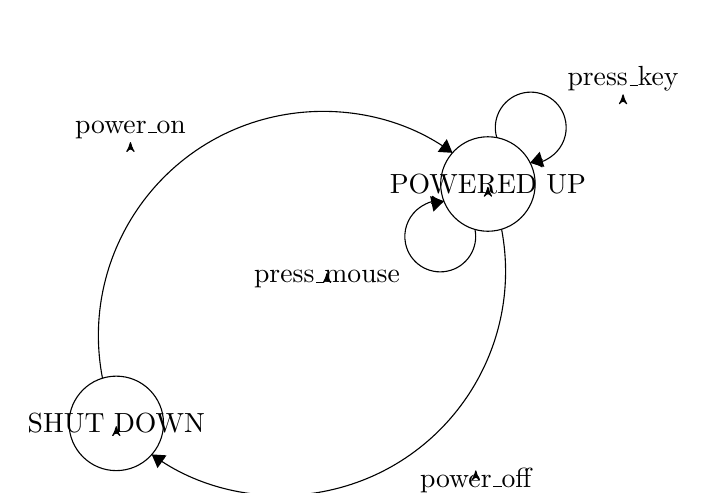
\begin{tikzpicture}[scale=0.2]
\tikzstyle{every node}+=[inner sep=0pt]
\draw [black] (27.8,-33.6) circle (3);
\draw (27.8,-33.6) node {SHUT DOWN};
\draw [black] (51.4,-18.4) circle (3);
\draw (51.4,-18.4) node {POWERED UP};
\draw [black] (26.925,-30.736) arc (-169.04911:-305.38232:14.242);
\fill [black] (49.15,-16.42) -- (48.79,-15.55) -- (48.21,-16.36);
\draw (28.7,-15.56) node [above] {power\_on};
\draw [black] (52.267,-21.266) arc (10.79218:-125.22362:14.249);
\fill [black] (30.05,-35.57) -- (30.42,-36.44) -- (30.99,-35.63);
\draw (50.63,-36.41) node [below] {power\_off};
\draw [black] (51.966,-15.466) arc (196.80695:-91.19305:2.25);
\draw (59.98,-12.53) node [above] {press\_key};
\fill [black] (54.07,-17.06) -- (54.98,-17.31) -- (54.69,-16.35);
\draw [black] (50.576,-21.272) arc (11.72631:-276.27369:2.25);
\draw (41.18,-23.88) node [below] {press\_mouse};
\fill [black] (48.62,-19.49) -- (47.73,-19.17) -- (47.94,-20.15);
\end{tikzpicture}
\end{center}

\subsection{A Process Algebra}
We next introduce our process algebra. Because for the moment we will only give a syntactic definition, we will have to rely on a set of equations that conform our denotational semantics. These rules will not be given here and instead we will give the transformation from each operator and construct of process algebra to its equivalent LTS structure.
%TODO Arreglar ecuaciones


Throughout this section we will use $ P $ to denote the set of processes.
\subsubsection{Sequential Processes}
Next we see the basic ways of composing processes.
\begin{definition} [Sequential composition]
	Let $ p, q \in P $. The sequential composition of $ p $ and $ q $, $ p \cdot q $, is a process that runs the process $ p $ and after finishing it runs the process $ q $. The operator is usually omitted if there is no contextual ambiguity, writing the composition as $ pq $.
\end{definition}

Given the LTS denotation of $ p $ and $ q $, and supposing that $ p_F $ is the set of final states in the LTS of $ p $, and $ q_0 $ is the initial state of the LTS of $ q $, then their sequential composition will be represented by the LTS that ``fuses'' each element of $ p_F $ with $ q_0 $ thus introducing overlapped ``copies'' of the transitions of $ q_0 $ after every state of $ p_F $.
\begin{figure}[H]
	\minipage{0.32\textwidth}
	\centering
	
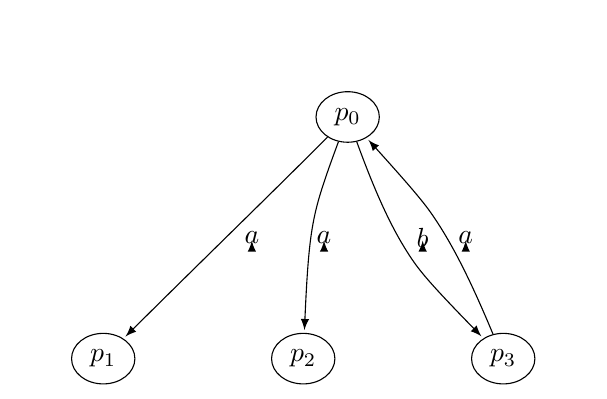
\begin{tikzpicture}[>=latex,line join=bevel,]
%%
\begin{scope}
  \pgfsetstrokecolor{black}
  \definecolor{strokecol}{rgb}{1.0,1.0,1.0};
  \pgfsetstrokecolor{strokecol}
  \definecolor{fillcol}{rgb}{1.0,1.0,1.0};
  \pgfsetfillcolor{fillcol}
  \filldraw (0.0bp,0.0bp) -- (0.0bp,123.0bp) -- (198.0bp,123.0bp) -- (198.0bp,0.0bp) -- cycle;
\end{scope}
  \node (p_2) at (99.0bp,18.0bp) [draw,ellipse] {$p_2$};
  \node (p_3) at (171.0bp,18.0bp) [draw,ellipse] {$p_3$};
  \node (p_0) at (115.0bp,105.0bp) [draw,ellipse] {$p_0$};
  \node (p_1) at (27.0bp,18.0bp) [draw,ellipse] {$p_1$};
  \draw [->] (p_3) ..controls (159.4bp,45.816bp) and (153.06bp,58.546bp)  .. (146.0bp,69.0bp) .. controls (143.06bp,73.344bp) and (139.64bp,77.725bp)  .. (p_0);
  \definecolor{strokecol}{rgb}{0.0,0.0,0.0};
  \pgfsetstrokecolor{strokecol}
  \draw (157.5bp,61.5bp) node {$a$};
  \draw [->] (p_0) ..controls (106.34bp,81.737bp) and (104.28bp,75.163bp)  .. (103.0bp,69.0bp) .. controls (101.48bp,61.698bp) and (100.53bp,53.686bp)  .. (p_2);
  \draw (106.5bp,61.5bp) node {$a$};
  \draw [->] (p_0) ..controls (86.081bp,76.067bp) and (64.992bp,55.697bp)  .. (p_1);
  \draw (80.5bp,61.5bp) node {$a$};
  \draw [->] (p_0) ..controls (125.23bp,77.03bp) and (131.05bp,64.297bp)  .. (138.0bp,54.0bp) .. controls (141.15bp,49.327bp) and (144.94bp,44.685bp)  .. (p_3);
  \draw (142.0bp,61.5bp) node {$b$};
%
\end{tikzpicture}

	\caption{LTS of P} \label{fig:SequentialCompositionP}
	\endminipage\hfill
	\minipage{0.32\textwidth}
	\centering
	
\begin{tikzpicture}[>=latex,line join=bevel,]
%%
\node (q_7) at (99.0bp,18.0bp) [draw,ellipse] {$q_7$};
  \node (q_6) at (243.0bp,105.0bp) [draw,ellipse] {$q_6$};
  \node (q_5) at (171.0bp,105.0bp) [draw,ellipse] {$q_5$};
  \node (q_4) at (99.0bp,105.0bp) [draw,ellipse] {$q_4$};
  \node (q_3) at (27.0bp,105.0bp) [draw,ellipse] {$q_3$};
  \node (q_2) at (171.0bp,192.0bp) [draw,ellipse] {$q_2$};
  \node (q_1) at (99.0bp,192.0bp) [draw,ellipse] {$q_1$};
  \node (q_0) at (140.0bp,279.0bp) [draw,ellipse] {$q_0$};
  \node (q_8) at (171.0bp,18.0bp) [draw,ellipse] {$q_8$};
  \draw [->] (q_1) ..controls (75.07bp,162.75bp) and (58.964bp,143.74bp)  .. (q_3);
  \definecolor{strokecol}{rgb}{0.0,0.0,0.0};
  \pgfsetstrokecolor{strokecol}
  \draw (72.0bp,148.5bp) node {$b$};
  \draw [->] (q_4) ..controls (99.0bp,75.163bp) and (99.0bp,59.548bp)  .. (q_7);
  \draw (102.5bp,61.5bp) node {$e$};
  \draw [->] (q_0) ..controls (126.2bp,249.38bp) and (118.03bp,232.44bp)  .. (q_1);
  \draw (125.5bp,235.5bp) node {$a$};
  \draw [->] (q_1) ..controls (99.0bp,162.16bp) and (99.0bp,146.55bp)  .. (q_4);
  \draw (102.5bp,148.5bp) node {$c$};
  \draw [->] (q_0) ..controls (150.5bp,249.22bp) and (156.47bp,232.85bp)  .. (q_2);
  \draw (161.5bp,235.5bp) node {$a$};
  \draw [->] (q_5) ..controls (171.0bp,75.163bp) and (171.0bp,59.548bp)  .. (q_8);
  \draw (175.0bp,61.5bp) node {$d$};
  \draw [->] (q_2) ..controls (194.93bp,162.75bp) and (211.04bp,143.74bp)  .. (q_6);
  \draw (214.5bp,148.5bp) node {$f$};
  \draw [->] (q_2) ..controls (171.0bp,162.16bp) and (171.0bp,146.55bp)  .. (q_5);
  \draw (174.5bp,148.5bp) node {$c$};
%
\end{tikzpicture}

	\caption{LTS of Q} \label{fig:SequentialCompositionP}
	\endminipage\hfill
	\minipage{0.32\textwidth}
	\centering
	
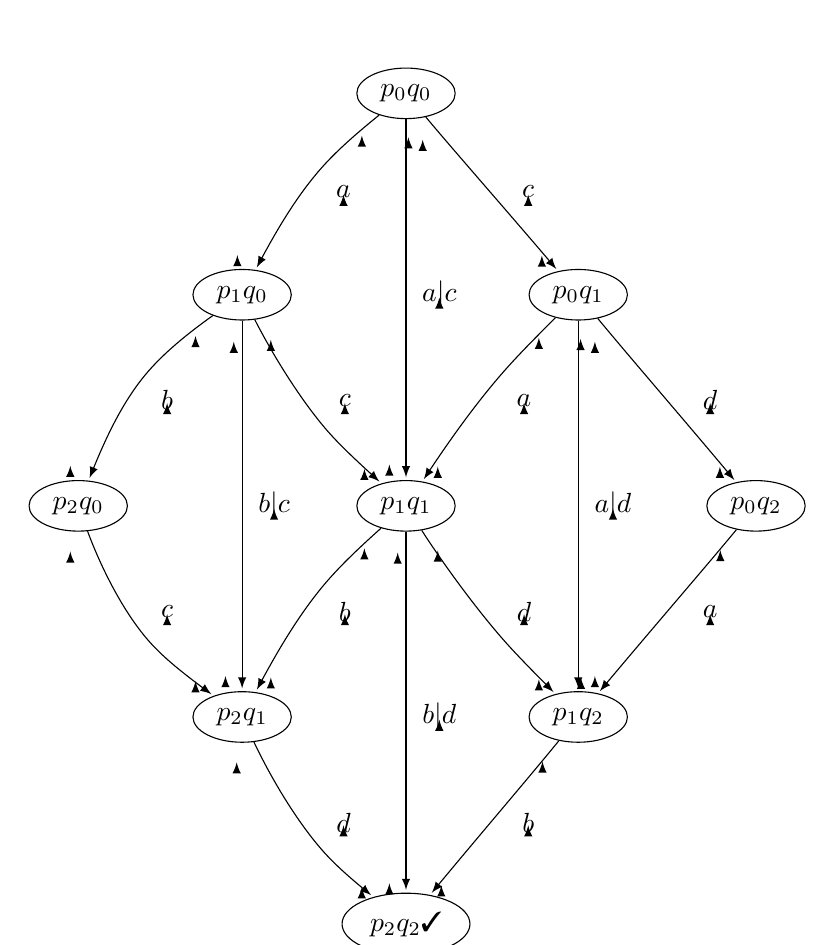
\begin{tikzpicture}[>=latex,line join=bevel,]
%%
\begin{scope}
  \pgfsetstrokecolor{black}
  \definecolor{strokecol}{rgb}{1.0,1.0,1.0};
  \pgfsetstrokecolor{strokecol}
  \definecolor{fillcol}{rgb}{1.0,1.0,1.0};
  \pgfsetfillcolor{fillcol}
  \filldraw (0.0bp,0.0bp) -- (0.0bp,318.0bp) -- (280.0bp,318.0bp) -- (280.0bp,0.0bp) -- cycle;
\end{scope}
\begin{scope}
  \pgfsetstrokecolor{black}
  \definecolor{strokecol}{rgb}{1.0,1.0,1.0};
  \pgfsetstrokecolor{strokecol}
  \definecolor{fillcol}{rgb}{1.0,1.0,1.0};
  \pgfsetfillcolor{fillcol}
  \filldraw (0.0bp,0.0bp) -- (0.0bp,318.0bp) -- (280.0bp,318.0bp) -- (280.0bp,0.0bp) -- cycle;
\end{scope}
\begin{scope}
  \pgfsetstrokecolor{black}
  \definecolor{strokecol}{rgb}{1.0,1.0,1.0};
  \pgfsetstrokecolor{strokecol}
  \definecolor{fillcol}{rgb}{1.0,1.0,1.0};
  \pgfsetfillcolor{fillcol}
  \filldraw (0.0bp,0.0bp) -- (0.0bp,318.0bp) -- (280.0bp,318.0bp) -- (280.0bp,0.0bp) -- cycle;
\end{scope}
  \node (p_1q_2) at (198.0bp,84.0bp) [draw,ellipse] {$p_1q_2$};
  \node (p_2q_1) at (77.0bp,84.0bp) [draw,ellipse] {$p_2q_1$};
  \node (p_1q_0) at (77.0bp,236.0bp) [draw,ellipse] {$p_1q_0$};
  \node (p_2q_0) at (18.0bp,160.0bp) [draw,ellipse] {$p_2q_0$};
  \node (p_1q_1) at (136.0bp,160.0bp) [draw,ellipse] {$p_1q_1$};
  \node (p_0q_1) at (198.0bp,236.0bp) [draw,ellipse] {$p_0q_1$};
  \node (p_0q_0) at (136.0bp,308.5bp) [draw,ellipse] {$p_0q_0$};
  \node (p_0q_2) at (262.0bp,160.0bp) [draw,ellipse] {$p_0q_2$};
  \node (p_2q_2) at (136.0bp,9.5bp) [draw,ellipse] {$p_2 q_2 \text{\cmark}$};
  \draw [->] (p_2q_1) ..controls (85.943bp,65.034bp) and (94.82bp,48.961bp)  .. (105.0bp,37.0bp) .. controls (108.9bp,32.417bp) and (113.63bp,27.956bp)  .. (p_2q_2);
  \definecolor{strokecol}{rgb}{0.0,0.0,0.0};
  \pgfsetstrokecolor{strokecol}
  \draw (113.5bp,46.0bp) node {$d$};
  \draw (75.042bp,68.67bp) node {$$};
  \draw (120.07bp,23.676bp) node {$$};
  \draw [->] (p_1q_0) ..controls (86.56bp,217.21bp) and (95.89bp,201.22bp)  .. (106.0bp,189.0bp) .. controls (109.97bp,184.2bp) and (114.74bp,179.41bp)  .. (p_1q_1);
  \draw (114.0bp,198.0bp) node {$c$};
  \draw (87.34bp,220.76bp) node {$$};
  \draw (121.02bp,174.3bp) node {$$};
  \draw [->] (p_1q_0) ..controls (77.0bp,202.14bp) and (77.0bp,136.25bp)  .. (p_2q_1);
  \draw (88.5bp,160.0bp) node {$b|c$};
  \draw (74.0bp,220.07bp) node {$$};
  \draw (71.0bp,99.699bp) node {$$};
  \draw [->] (p_1q_2) ..controls (181.11bp,63.253bp) and (162.3bp,41.26bp)  .. (p_2q_2);
  \draw (180.0bp,46.0bp) node {$b$};
  \draw (185.13bp,68.964bp) node {$$};
  \draw (148.71bp,24.351bp) node {$$};
  \draw [->] (p_1q_1) ..controls (120.73bp,146.34bp) and (112.36bp,138.69bp)  .. (106.0bp,131.0bp) .. controls (98.575bp,122.03bp) and (91.572bp,111.02bp)  .. (p_2q_1);
  \draw (114.0bp,122.0bp) node {$b$};
  \draw (121.02bp,145.7bp) node {$$};
  \draw (87.34bp,99.238bp) node {$$};
  \draw [->] (p_0q_0) ..controls (136.0bp,275.62bp) and (136.0bp,212.22bp)  .. (p_1q_1);
  \draw (148.0bp,236.0bp) node {$a|c$};
  \draw (142.0bp,292.77bp) node {$$};
  \draw (130.0bp,175.87bp) node {$$};
  \draw [->] (p_0q_2) ..controls (244.81bp,139.13bp) and (225.01bp,116.23bp)  .. (p_1q_2);
  \draw (245.5bp,122.0bp) node {$a$};
  \draw (249.15bp,145.08bp) node {$$};
  \draw (198.99bp,99.087bp) node {$$};
  \draw [->] (p_1q_1) ..controls (147.87bp,141.5bp) and (159.11bp,125.64bp)  .. (170.0bp,113.0bp) .. controls (173.83bp,108.56bp) and (178.21bp,103.96bp)  .. (p_1q_2);
  \draw (178.5bp,122.0bp) node {$d$};
  \draw (147.43bp,144.91bp) node {$$};
  \draw (183.83bp,98.545bp) node {$$};
  \draw [->] (p_1q_1) ..controls (136.0bp,126.58bp) and (136.0bp,61.809bp)  .. (p_2q_2);
  \draw (148.0bp,84.0bp) node {$b|d$};
  \draw (133.0bp,144.16bp) node {$$};
  \draw (130.0bp,25.112bp) node {$$};
  \draw [->] (p_2q_0) ..controls (25.054bp,140.84bp) and (32.385bp,124.69bp)  .. (42.0bp,113.0bp) .. controls (46.542bp,107.48bp) and (52.332bp,102.31bp)  .. (p_2q_1);
  \draw (50.0bp,122.0bp) node {$c$};
  \draw (15.15bp,144.57bp) node {$$};
  \draw (60.217bp,97.855bp) node {$$};
  \draw [->] (p_0q_0) ..controls (119.67bp,295.29bp) and (111.31bp,288.27bp)  .. (105.0bp,281.0bp) .. controls (97.916bp,272.84bp) and (91.354bp,262.73bp)  .. (p_1q_0);
  \draw (113.5bp,273.0bp) node {$a$};
  \draw (120.11bp,294.28bp) node {$$};
  \draw (75.294bp,251.28bp) node {$$};
  \draw [->] (p_0q_0) ..controls (152.78bp,288.42bp) and (171.3bp,267.36bp)  .. (p_0q_1);
  \draw (180.0bp,273.0bp) node {$c$};
  \draw (136.87bp,293.69bp) node {$$};
  \draw (184.91bp,251.07bp) node {$$};
  \draw [->] (p_0q_1) ..controls (198.0bp,202.14bp) and (198.0bp,136.25bp)  .. (p_1q_2);
  \draw (210.5bp,160.0bp) node {$a|d$};
  \draw (204.0bp,220.07bp) node {$$};
  \draw (204.0bp,99.699bp) node {$$};
  \draw [->] (p_0q_1) ..controls (215.19bp,215.13bp) and (234.99bp,192.23bp)  .. (p_0q_2);
  \draw (245.5bp,198.0bp) node {$d$};
  \draw (198.85bp,221.08bp) node {$$};
  \draw (249.01bp,175.09bp) node {$$};
  \draw [->] (p_0q_1) ..controls (184.07bp,221.98bp) and (176.28bp,214.29bp)  .. (170.0bp,207.0bp) .. controls (161.92bp,197.62bp) and (153.64bp,186.46bp)  .. (p_1q_1);
  \draw (178.5bp,198.0bp) node {$a$};
  \draw (183.83bp,221.46bp) node {$$};
  \draw (147.43bp,175.09bp) node {$$};
  \draw [->] (p_1q_0) ..controls (58.74bp,223.0bp) and (48.922bp,215.41bp)  .. (42.0bp,207.0bp) .. controls (35.014bp,198.51bp) and (29.234bp,187.66bp)  .. (p_2q_0);
  \draw (50.0bp,198.0bp) node {$b$};
  \draw (60.217bp,222.14bp) node {$$};
  \draw (15.15bp,175.43bp) node {$$};
%
\end{tikzpicture}

	\caption{LTS of P·Q} \label{fig:SequentialCompositionP}
	\endminipage\hfill
\end{figure}

\begin{definition} [Alternative composition]
	Let $ p, q \in P$. The alternative composition of $ p $ and $ q $, $ p + q $, is a process that either runs $ p $ or $ q $. This operator is also called the choice operator.
\end{definition}

The choice of processes $ p $ and $ q $ is translated to an LTS where the initial states $ p_0 $ and $ q_0 $ are fused, creating a new initial state which is the source of the transitions of the previous initial states. However, $ p_0 $ and $ q_0 $ are also preserved, as the initial choice is only made once, but we must preserve the possible loops of each individual process.

\begin{figure}[H]
	\minipage{0.5\textwidth}
	\centering
	
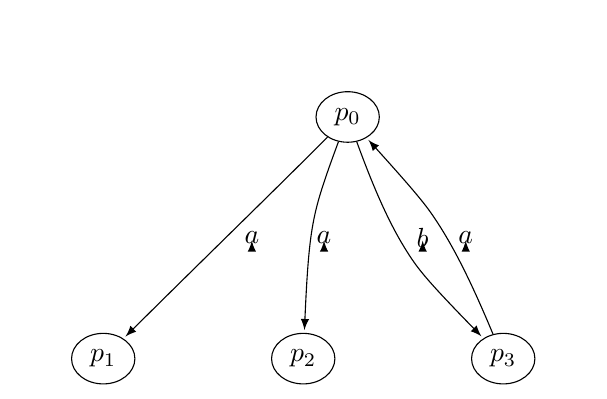
\begin{tikzpicture}[>=latex,line join=bevel,]
%%
\begin{scope}
  \pgfsetstrokecolor{black}
  \definecolor{strokecol}{rgb}{1.0,1.0,1.0};
  \pgfsetstrokecolor{strokecol}
  \definecolor{fillcol}{rgb}{1.0,1.0,1.0};
  \pgfsetfillcolor{fillcol}
  \filldraw (0.0bp,0.0bp) -- (0.0bp,123.0bp) -- (198.0bp,123.0bp) -- (198.0bp,0.0bp) -- cycle;
\end{scope}
  \node (p_2) at (99.0bp,18.0bp) [draw,ellipse] {$p_2$};
  \node (p_3) at (171.0bp,18.0bp) [draw,ellipse] {$p_3$};
  \node (p_0) at (115.0bp,105.0bp) [draw,ellipse] {$p_0$};
  \node (p_1) at (27.0bp,18.0bp) [draw,ellipse] {$p_1$};
  \draw [->] (p_3) ..controls (159.4bp,45.816bp) and (153.06bp,58.546bp)  .. (146.0bp,69.0bp) .. controls (143.06bp,73.344bp) and (139.64bp,77.725bp)  .. (p_0);
  \definecolor{strokecol}{rgb}{0.0,0.0,0.0};
  \pgfsetstrokecolor{strokecol}
  \draw (157.5bp,61.5bp) node {$a$};
  \draw [->] (p_0) ..controls (106.34bp,81.737bp) and (104.28bp,75.163bp)  .. (103.0bp,69.0bp) .. controls (101.48bp,61.698bp) and (100.53bp,53.686bp)  .. (p_2);
  \draw (106.5bp,61.5bp) node {$a$};
  \draw [->] (p_0) ..controls (86.081bp,76.067bp) and (64.992bp,55.697bp)  .. (p_1);
  \draw (80.5bp,61.5bp) node {$a$};
  \draw [->] (p_0) ..controls (125.23bp,77.03bp) and (131.05bp,64.297bp)  .. (138.0bp,54.0bp) .. controls (141.15bp,49.327bp) and (144.94bp,44.685bp)  .. (p_3);
  \draw (142.0bp,61.5bp) node {$b$};
%
\end{tikzpicture}

	\caption{LTS of P} \label{fig:AlternativeCompositionP}
	\endminipage\hfill
	\minipage{0.5\textwidth}
	\centering
	
\begin{tikzpicture}[>=latex,line join=bevel,]
%%
\node (q_7) at (99.0bp,18.0bp) [draw,ellipse] {$q_7$};
  \node (q_6) at (243.0bp,105.0bp) [draw,ellipse] {$q_6$};
  \node (q_5) at (171.0bp,105.0bp) [draw,ellipse] {$q_5$};
  \node (q_4) at (99.0bp,105.0bp) [draw,ellipse] {$q_4$};
  \node (q_3) at (27.0bp,105.0bp) [draw,ellipse] {$q_3$};
  \node (q_2) at (171.0bp,192.0bp) [draw,ellipse] {$q_2$};
  \node (q_1) at (99.0bp,192.0bp) [draw,ellipse] {$q_1$};
  \node (q_0) at (140.0bp,279.0bp) [draw,ellipse] {$q_0$};
  \node (q_8) at (171.0bp,18.0bp) [draw,ellipse] {$q_8$};
  \draw [->] (q_1) ..controls (75.07bp,162.75bp) and (58.964bp,143.74bp)  .. (q_3);
  \definecolor{strokecol}{rgb}{0.0,0.0,0.0};
  \pgfsetstrokecolor{strokecol}
  \draw (72.0bp,148.5bp) node {$b$};
  \draw [->] (q_4) ..controls (99.0bp,75.163bp) and (99.0bp,59.548bp)  .. (q_7);
  \draw (102.5bp,61.5bp) node {$e$};
  \draw [->] (q_0) ..controls (126.2bp,249.38bp) and (118.03bp,232.44bp)  .. (q_1);
  \draw (125.5bp,235.5bp) node {$a$};
  \draw [->] (q_1) ..controls (99.0bp,162.16bp) and (99.0bp,146.55bp)  .. (q_4);
  \draw (102.5bp,148.5bp) node {$c$};
  \draw [->] (q_0) ..controls (150.5bp,249.22bp) and (156.47bp,232.85bp)  .. (q_2);
  \draw (161.5bp,235.5bp) node {$a$};
  \draw [->] (q_5) ..controls (171.0bp,75.163bp) and (171.0bp,59.548bp)  .. (q_8);
  \draw (175.0bp,61.5bp) node {$d$};
  \draw [->] (q_2) ..controls (194.93bp,162.75bp) and (211.04bp,143.74bp)  .. (q_6);
  \draw (214.5bp,148.5bp) node {$f$};
  \draw [->] (q_2) ..controls (171.0bp,162.16bp) and (171.0bp,146.55bp)  .. (q_5);
  \draw (174.5bp,148.5bp) node {$c$};
%
\end{tikzpicture}

	\caption{LTS of Q} \label{fig:AlternativeCompositionQ}
	\endminipage\hfill
\end{figure}
\begin{figure} [H]
	\centering
	
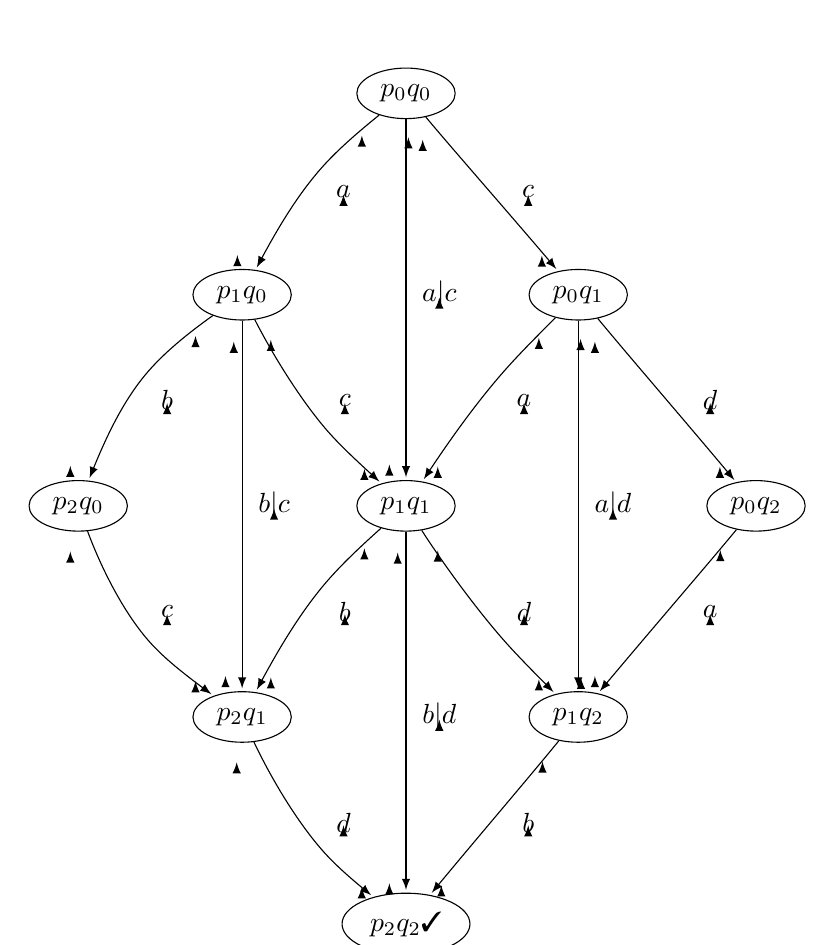
\begin{tikzpicture}[>=latex,line join=bevel,]
%%
\begin{scope}
  \pgfsetstrokecolor{black}
  \definecolor{strokecol}{rgb}{1.0,1.0,1.0};
  \pgfsetstrokecolor{strokecol}
  \definecolor{fillcol}{rgb}{1.0,1.0,1.0};
  \pgfsetfillcolor{fillcol}
  \filldraw (0.0bp,0.0bp) -- (0.0bp,318.0bp) -- (280.0bp,318.0bp) -- (280.0bp,0.0bp) -- cycle;
\end{scope}
\begin{scope}
  \pgfsetstrokecolor{black}
  \definecolor{strokecol}{rgb}{1.0,1.0,1.0};
  \pgfsetstrokecolor{strokecol}
  \definecolor{fillcol}{rgb}{1.0,1.0,1.0};
  \pgfsetfillcolor{fillcol}
  \filldraw (0.0bp,0.0bp) -- (0.0bp,318.0bp) -- (280.0bp,318.0bp) -- (280.0bp,0.0bp) -- cycle;
\end{scope}
\begin{scope}
  \pgfsetstrokecolor{black}
  \definecolor{strokecol}{rgb}{1.0,1.0,1.0};
  \pgfsetstrokecolor{strokecol}
  \definecolor{fillcol}{rgb}{1.0,1.0,1.0};
  \pgfsetfillcolor{fillcol}
  \filldraw (0.0bp,0.0bp) -- (0.0bp,318.0bp) -- (280.0bp,318.0bp) -- (280.0bp,0.0bp) -- cycle;
\end{scope}
  \node (p_1q_2) at (198.0bp,84.0bp) [draw,ellipse] {$p_1q_2$};
  \node (p_2q_1) at (77.0bp,84.0bp) [draw,ellipse] {$p_2q_1$};
  \node (p_1q_0) at (77.0bp,236.0bp) [draw,ellipse] {$p_1q_0$};
  \node (p_2q_0) at (18.0bp,160.0bp) [draw,ellipse] {$p_2q_0$};
  \node (p_1q_1) at (136.0bp,160.0bp) [draw,ellipse] {$p_1q_1$};
  \node (p_0q_1) at (198.0bp,236.0bp) [draw,ellipse] {$p_0q_1$};
  \node (p_0q_0) at (136.0bp,308.5bp) [draw,ellipse] {$p_0q_0$};
  \node (p_0q_2) at (262.0bp,160.0bp) [draw,ellipse] {$p_0q_2$};
  \node (p_2q_2) at (136.0bp,9.5bp) [draw,ellipse] {$p_2 q_2 \text{\cmark}$};
  \draw [->] (p_2q_1) ..controls (85.943bp,65.034bp) and (94.82bp,48.961bp)  .. (105.0bp,37.0bp) .. controls (108.9bp,32.417bp) and (113.63bp,27.956bp)  .. (p_2q_2);
  \definecolor{strokecol}{rgb}{0.0,0.0,0.0};
  \pgfsetstrokecolor{strokecol}
  \draw (113.5bp,46.0bp) node {$d$};
  \draw (75.042bp,68.67bp) node {$$};
  \draw (120.07bp,23.676bp) node {$$};
  \draw [->] (p_1q_0) ..controls (86.56bp,217.21bp) and (95.89bp,201.22bp)  .. (106.0bp,189.0bp) .. controls (109.97bp,184.2bp) and (114.74bp,179.41bp)  .. (p_1q_1);
  \draw (114.0bp,198.0bp) node {$c$};
  \draw (87.34bp,220.76bp) node {$$};
  \draw (121.02bp,174.3bp) node {$$};
  \draw [->] (p_1q_0) ..controls (77.0bp,202.14bp) and (77.0bp,136.25bp)  .. (p_2q_1);
  \draw (88.5bp,160.0bp) node {$b|c$};
  \draw (74.0bp,220.07bp) node {$$};
  \draw (71.0bp,99.699bp) node {$$};
  \draw [->] (p_1q_2) ..controls (181.11bp,63.253bp) and (162.3bp,41.26bp)  .. (p_2q_2);
  \draw (180.0bp,46.0bp) node {$b$};
  \draw (185.13bp,68.964bp) node {$$};
  \draw (148.71bp,24.351bp) node {$$};
  \draw [->] (p_1q_1) ..controls (120.73bp,146.34bp) and (112.36bp,138.69bp)  .. (106.0bp,131.0bp) .. controls (98.575bp,122.03bp) and (91.572bp,111.02bp)  .. (p_2q_1);
  \draw (114.0bp,122.0bp) node {$b$};
  \draw (121.02bp,145.7bp) node {$$};
  \draw (87.34bp,99.238bp) node {$$};
  \draw [->] (p_0q_0) ..controls (136.0bp,275.62bp) and (136.0bp,212.22bp)  .. (p_1q_1);
  \draw (148.0bp,236.0bp) node {$a|c$};
  \draw (142.0bp,292.77bp) node {$$};
  \draw (130.0bp,175.87bp) node {$$};
  \draw [->] (p_0q_2) ..controls (244.81bp,139.13bp) and (225.01bp,116.23bp)  .. (p_1q_2);
  \draw (245.5bp,122.0bp) node {$a$};
  \draw (249.15bp,145.08bp) node {$$};
  \draw (198.99bp,99.087bp) node {$$};
  \draw [->] (p_1q_1) ..controls (147.87bp,141.5bp) and (159.11bp,125.64bp)  .. (170.0bp,113.0bp) .. controls (173.83bp,108.56bp) and (178.21bp,103.96bp)  .. (p_1q_2);
  \draw (178.5bp,122.0bp) node {$d$};
  \draw (147.43bp,144.91bp) node {$$};
  \draw (183.83bp,98.545bp) node {$$};
  \draw [->] (p_1q_1) ..controls (136.0bp,126.58bp) and (136.0bp,61.809bp)  .. (p_2q_2);
  \draw (148.0bp,84.0bp) node {$b|d$};
  \draw (133.0bp,144.16bp) node {$$};
  \draw (130.0bp,25.112bp) node {$$};
  \draw [->] (p_2q_0) ..controls (25.054bp,140.84bp) and (32.385bp,124.69bp)  .. (42.0bp,113.0bp) .. controls (46.542bp,107.48bp) and (52.332bp,102.31bp)  .. (p_2q_1);
  \draw (50.0bp,122.0bp) node {$c$};
  \draw (15.15bp,144.57bp) node {$$};
  \draw (60.217bp,97.855bp) node {$$};
  \draw [->] (p_0q_0) ..controls (119.67bp,295.29bp) and (111.31bp,288.27bp)  .. (105.0bp,281.0bp) .. controls (97.916bp,272.84bp) and (91.354bp,262.73bp)  .. (p_1q_0);
  \draw (113.5bp,273.0bp) node {$a$};
  \draw (120.11bp,294.28bp) node {$$};
  \draw (75.294bp,251.28bp) node {$$};
  \draw [->] (p_0q_0) ..controls (152.78bp,288.42bp) and (171.3bp,267.36bp)  .. (p_0q_1);
  \draw (180.0bp,273.0bp) node {$c$};
  \draw (136.87bp,293.69bp) node {$$};
  \draw (184.91bp,251.07bp) node {$$};
  \draw [->] (p_0q_1) ..controls (198.0bp,202.14bp) and (198.0bp,136.25bp)  .. (p_1q_2);
  \draw (210.5bp,160.0bp) node {$a|d$};
  \draw (204.0bp,220.07bp) node {$$};
  \draw (204.0bp,99.699bp) node {$$};
  \draw [->] (p_0q_1) ..controls (215.19bp,215.13bp) and (234.99bp,192.23bp)  .. (p_0q_2);
  \draw (245.5bp,198.0bp) node {$d$};
  \draw (198.85bp,221.08bp) node {$$};
  \draw (249.01bp,175.09bp) node {$$};
  \draw [->] (p_0q_1) ..controls (184.07bp,221.98bp) and (176.28bp,214.29bp)  .. (170.0bp,207.0bp) .. controls (161.92bp,197.62bp) and (153.64bp,186.46bp)  .. (p_1q_1);
  \draw (178.5bp,198.0bp) node {$a$};
  \draw (183.83bp,221.46bp) node {$$};
  \draw (147.43bp,175.09bp) node {$$};
  \draw [->] (p_1q_0) ..controls (58.74bp,223.0bp) and (48.922bp,215.41bp)  .. (42.0bp,207.0bp) .. controls (35.014bp,198.51bp) and (29.234bp,187.66bp)  .. (p_2q_0);
  \draw (50.0bp,198.0bp) node {$b$};
  \draw (60.217bp,222.14bp) node {$$};
  \draw (15.15bp,175.43bp) node {$$};
%
\end{tikzpicture}

	\caption{LTS of P+Q} \label{fig:AlternativeCompositionPQ}
\end{figure}


\begin{definition} [\textit{Deadlock}]
	The process \textit{deadlock}, denoted by $ \sigma $, is a process that cannot do anything at all, but this includes that it cannot terminate, either.
\end{definition}
\textit{Deadlock} is not usually used as a ``desired'' component of a process, but rather as the state a process reaches when any uncontrollable error happens or we arrive to the typical deadlock situation where a miscommunication between several components is produced. In fact, the translation of the \textit{deadlock} process is the LTS with a single non-terminating state without transitions.
\begin{figure} [H]
	\centering
	
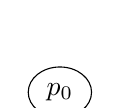
\begin{tikzpicture}[>=latex,line join=bevel,]
%%
\node (p_0) at (11.5bp,9.5bp) [draw,ellipse] {$p_0$};
%
\end{tikzpicture}

	\caption{LTS of $\delta$} \label{fig:DeadlockDelta}
\end{figure}
\begin{definition} [Conditional operator]
	Let $ c \in \rm I\!B $, $ p, q \in P$. The conditional operator $ c\rightarrow p \diamond q $ behaves as $ p $ if $ c $ is true, or as $ q $, otherwise.
\end{definition}
Conditional operators are especially useful for specifying different behaviors of parameterized processes that depend on the value of the parameters. By using this operator, one can describe general processes that capture a single abstract behavior, even if the concrete behavior depends on a certain conditions on their parameters.

As an example, we can consider the \textit{factorial(n)} process, which calculates $ n! $. Using the common recursive definition, we need a base case, which will be implemented by a conditional operator.

\begin{figure} [H]
	\centering
	
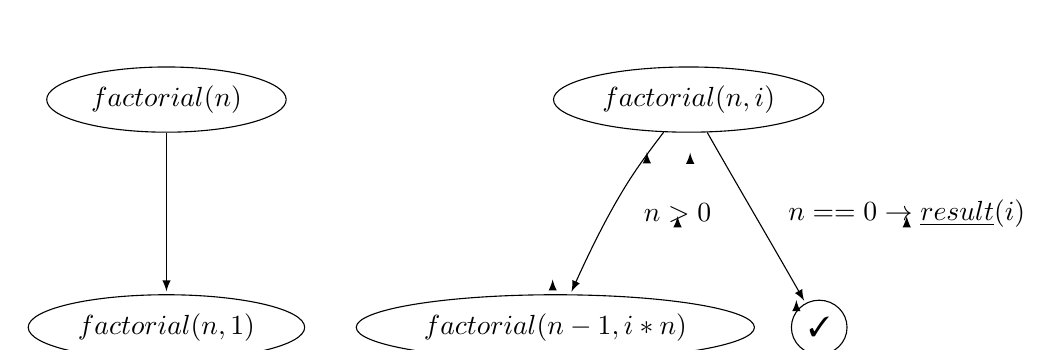
\begin{tikzpicture}[>=latex,line join=bevel,]
%%
\node (factorial_n) at (50.0bp,94.0bp) [draw,ellipse] {$factorial(n)$};
  \node (factorial_n_i) at (238.0bp,94.0bp) [draw,ellipse] {$factorial(n,i)$};
  \node (factorial_n_1_i_n) at (190.0bp,12.0bp) [draw,ellipse] {$factorial(n-1,i*n)$};
  \node (result_i) at (285.0bp,12.0bp) [draw,ellipse] {$\text{\cmark}$};
  \node (factorial_n_1) at (50.0bp,12.0bp) [draw,ellipse] {$factorial(n,1)$};
  \draw [->] (factorial_n_i) ..controls (224.78bp,76.747bp) and (219.9bp,70.21bp)  .. (216.0bp,64.0bp) .. controls (209.89bp,54.252bp) and (203.98bp,42.89bp)  .. (factorial_n_1_i_n);
  \definecolor{strokecol}{rgb}{0.0,0.0,0.0};
  \pgfsetstrokecolor{strokecol}
  \draw (234.0bp,53.0bp) node {$n>0$};
  \draw (222.95bp,76.039bp) node {$$};
  \draw (189.03bp,30.254bp) node {$$};
  \draw [->] (factorial_n_i) ..controls (253.22bp,67.086bp) and (268.54bp,41.017bp)  .. (result_i);
  \draw (316.5bp,53.0bp) node {$n==0\rightarrow\underline{result}(i)$};
  \draw (238.54bp,75.876bp) node {$$};
  \draw (276.77bp,22.791bp) node {$$};
  \draw [->] (factorial_n) ..controls (50.0bp,69.577bp) and (50.0bp,49.479bp)  .. (factorial_n_1);
%
\end{tikzpicture}

	\caption{LTS of $factorial(n)$} \label{fig:ConditionalFactorial}
\end{figure}
\begin{definition} [Sum operator]
	The sum operator $ \sum_{d:D} p(d) $ generalizes the choice operator for actions parameterized with data in arbitrary domains.
\end{definition}

This operator lets us choose over a possibly infinite number of processes. The equivalent LTS construction is analogous to the binary sum one.


\subsubsection{Recursive Processes}
Processes are not always finite, and many systems need recursive definitions. These definitions are written as equations, that represent the relations that the instances of the (parameterized) process must satisfy. For example, \textit{factorial(n,i)} process is recursively defined as follows:
\begin{table}[H]
	\centering
	\begin{tabular}{  r@{ = }l  }
		$ factorial(n) $ & $ factorial(n,1) $ \\
		$ factorial(n,i) $ & $ i > 0 \rightarrow factorial(n-1,i*n) \diamond \underline{n} $
	\end{tabular}
\end{table}

This example shows what is called a \textit{recursive specification}, a set of process equations with only a single variable in each left-hand side. If every occurrence of a defined process variable at the right-hand side is preceded by an action, then we say that the recursive specification is \textit{guarded}, or that it is a \textit{guarded recursive specification}.

Guardedness is needed if we want to model sound systems. Any process defined by an unguarded recursive specification would contain a ``loop'' where no action is performed, and thus does not soundly define the behavior of a process.


\subsubsection{Parallel Processes}
\begin{definition} [Parallel composition]
	Let $ p, q \in P $. The parallel composition $ p \Vert q $ is a process in which actions from $ p $ and $ q $ happen independently from each other, but also simultaneously. The process terminates when both $ p $ and $ q $ terminate.
\end{definition}

Therefore, the parallel composition can perform actions from one process or the other, or both at the same time, without any order between them. \\
To facilitate the analysis of this operator, the following auxiliary operators are introduced.
\begin{definition} [Left-merge and right merge operators]
	Let $ p, q \in P $. The left-merge of $ p $ and $ q $, $ p \lfloor\!\lfloor q $, is the process that parallelizes $ p $ and $ q $, but guaranteeing that the first action will be from $ p $. Analogously, the right-merge $ p \rfloor\!\rfloor q $ ensures that the first action performed comes from $ q $.
\end{definition} 
\begin{definition} [Synchronization operator]
	Let $ p, q \in P $. The synchronization of $ p $ and $ q $, $ p\vert q $, is a parallelization of $ p $ and $ q $ that forces the simultaneous execution of some first actions of $ p $ and $ q $.
\end{definition}
It must be noticed that the synchronization operator (for processes) and the multiaction operator (for actions) are overloaded, the reason being that the meaning of both is ``the same'', but at different levels.

For two processes $ P $ and $ Q $, the LTS of $ P \Vert Q $ results by creating all (possible synchronized) combinations of their actions. Let us see an example to showcase the procedure.

Let $ P = a·b $ and $ Q = c·d $, then $ P \Vert Q = a·b \Vert c·d $. The LTS's are the following:
\begin{figure} [H]
	\minipage{0.5\textwidth}
	\centering
	
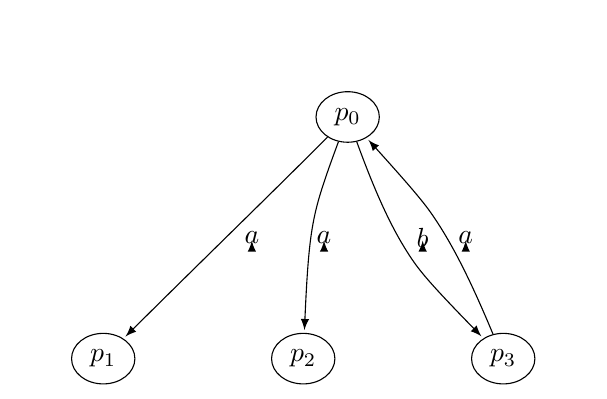
\begin{tikzpicture}[>=latex,line join=bevel,]
%%
\begin{scope}
  \pgfsetstrokecolor{black}
  \definecolor{strokecol}{rgb}{1.0,1.0,1.0};
  \pgfsetstrokecolor{strokecol}
  \definecolor{fillcol}{rgb}{1.0,1.0,1.0};
  \pgfsetfillcolor{fillcol}
  \filldraw (0.0bp,0.0bp) -- (0.0bp,123.0bp) -- (198.0bp,123.0bp) -- (198.0bp,0.0bp) -- cycle;
\end{scope}
  \node (p_2) at (99.0bp,18.0bp) [draw,ellipse] {$p_2$};
  \node (p_3) at (171.0bp,18.0bp) [draw,ellipse] {$p_3$};
  \node (p_0) at (115.0bp,105.0bp) [draw,ellipse] {$p_0$};
  \node (p_1) at (27.0bp,18.0bp) [draw,ellipse] {$p_1$};
  \draw [->] (p_3) ..controls (159.4bp,45.816bp) and (153.06bp,58.546bp)  .. (146.0bp,69.0bp) .. controls (143.06bp,73.344bp) and (139.64bp,77.725bp)  .. (p_0);
  \definecolor{strokecol}{rgb}{0.0,0.0,0.0};
  \pgfsetstrokecolor{strokecol}
  \draw (157.5bp,61.5bp) node {$a$};
  \draw [->] (p_0) ..controls (106.34bp,81.737bp) and (104.28bp,75.163bp)  .. (103.0bp,69.0bp) .. controls (101.48bp,61.698bp) and (100.53bp,53.686bp)  .. (p_2);
  \draw (106.5bp,61.5bp) node {$a$};
  \draw [->] (p_0) ..controls (86.081bp,76.067bp) and (64.992bp,55.697bp)  .. (p_1);
  \draw (80.5bp,61.5bp) node {$a$};
  \draw [->] (p_0) ..controls (125.23bp,77.03bp) and (131.05bp,64.297bp)  .. (138.0bp,54.0bp) .. controls (141.15bp,49.327bp) and (144.94bp,44.685bp)  .. (p_3);
  \draw (142.0bp,61.5bp) node {$b$};
%
\end{tikzpicture}

	\caption{LTS of $ P $} \label{fig:ParallelCompositionP}
	\endminipage\hfill
	\minipage{0.5\textwidth}
	\centering
	
\begin{tikzpicture}[>=latex,line join=bevel,]
%%
\node (q_7) at (99.0bp,18.0bp) [draw,ellipse] {$q_7$};
  \node (q_6) at (243.0bp,105.0bp) [draw,ellipse] {$q_6$};
  \node (q_5) at (171.0bp,105.0bp) [draw,ellipse] {$q_5$};
  \node (q_4) at (99.0bp,105.0bp) [draw,ellipse] {$q_4$};
  \node (q_3) at (27.0bp,105.0bp) [draw,ellipse] {$q_3$};
  \node (q_2) at (171.0bp,192.0bp) [draw,ellipse] {$q_2$};
  \node (q_1) at (99.0bp,192.0bp) [draw,ellipse] {$q_1$};
  \node (q_0) at (140.0bp,279.0bp) [draw,ellipse] {$q_0$};
  \node (q_8) at (171.0bp,18.0bp) [draw,ellipse] {$q_8$};
  \draw [->] (q_1) ..controls (75.07bp,162.75bp) and (58.964bp,143.74bp)  .. (q_3);
  \definecolor{strokecol}{rgb}{0.0,0.0,0.0};
  \pgfsetstrokecolor{strokecol}
  \draw (72.0bp,148.5bp) node {$b$};
  \draw [->] (q_4) ..controls (99.0bp,75.163bp) and (99.0bp,59.548bp)  .. (q_7);
  \draw (102.5bp,61.5bp) node {$e$};
  \draw [->] (q_0) ..controls (126.2bp,249.38bp) and (118.03bp,232.44bp)  .. (q_1);
  \draw (125.5bp,235.5bp) node {$a$};
  \draw [->] (q_1) ..controls (99.0bp,162.16bp) and (99.0bp,146.55bp)  .. (q_4);
  \draw (102.5bp,148.5bp) node {$c$};
  \draw [->] (q_0) ..controls (150.5bp,249.22bp) and (156.47bp,232.85bp)  .. (q_2);
  \draw (161.5bp,235.5bp) node {$a$};
  \draw [->] (q_5) ..controls (171.0bp,75.163bp) and (171.0bp,59.548bp)  .. (q_8);
  \draw (175.0bp,61.5bp) node {$d$};
  \draw [->] (q_2) ..controls (194.93bp,162.75bp) and (211.04bp,143.74bp)  .. (q_6);
  \draw (214.5bp,148.5bp) node {$f$};
  \draw [->] (q_2) ..controls (171.0bp,162.16bp) and (171.0bp,146.55bp)  .. (q_5);
  \draw (174.5bp,148.5bp) node {$c$};
%
\end{tikzpicture}

	\caption{LTS of $ Q $} \label{fig:ParallelCompositionQ}
	\endminipage\hfill
\end{figure}
\begin{figure} [H]
	\centering
	
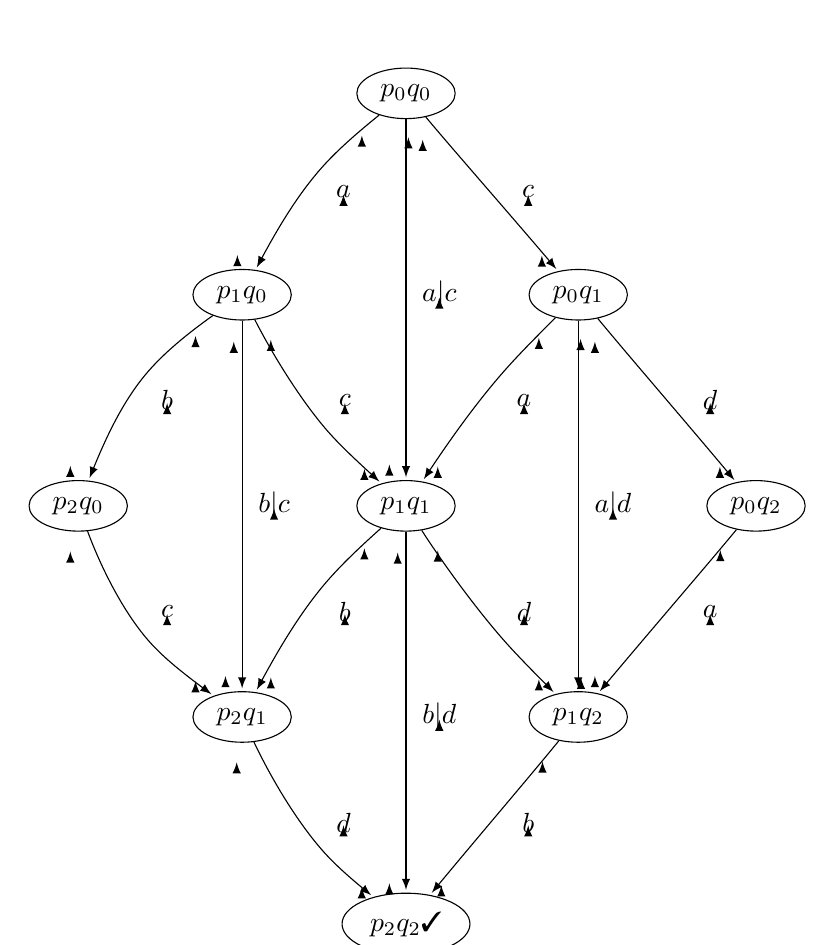
\begin{tikzpicture}[>=latex,line join=bevel,]
%%
\begin{scope}
  \pgfsetstrokecolor{black}
  \definecolor{strokecol}{rgb}{1.0,1.0,1.0};
  \pgfsetstrokecolor{strokecol}
  \definecolor{fillcol}{rgb}{1.0,1.0,1.0};
  \pgfsetfillcolor{fillcol}
  \filldraw (0.0bp,0.0bp) -- (0.0bp,318.0bp) -- (280.0bp,318.0bp) -- (280.0bp,0.0bp) -- cycle;
\end{scope}
\begin{scope}
  \pgfsetstrokecolor{black}
  \definecolor{strokecol}{rgb}{1.0,1.0,1.0};
  \pgfsetstrokecolor{strokecol}
  \definecolor{fillcol}{rgb}{1.0,1.0,1.0};
  \pgfsetfillcolor{fillcol}
  \filldraw (0.0bp,0.0bp) -- (0.0bp,318.0bp) -- (280.0bp,318.0bp) -- (280.0bp,0.0bp) -- cycle;
\end{scope}
\begin{scope}
  \pgfsetstrokecolor{black}
  \definecolor{strokecol}{rgb}{1.0,1.0,1.0};
  \pgfsetstrokecolor{strokecol}
  \definecolor{fillcol}{rgb}{1.0,1.0,1.0};
  \pgfsetfillcolor{fillcol}
  \filldraw (0.0bp,0.0bp) -- (0.0bp,318.0bp) -- (280.0bp,318.0bp) -- (280.0bp,0.0bp) -- cycle;
\end{scope}
  \node (p_1q_2) at (198.0bp,84.0bp) [draw,ellipse] {$p_1q_2$};
  \node (p_2q_1) at (77.0bp,84.0bp) [draw,ellipse] {$p_2q_1$};
  \node (p_1q_0) at (77.0bp,236.0bp) [draw,ellipse] {$p_1q_0$};
  \node (p_2q_0) at (18.0bp,160.0bp) [draw,ellipse] {$p_2q_0$};
  \node (p_1q_1) at (136.0bp,160.0bp) [draw,ellipse] {$p_1q_1$};
  \node (p_0q_1) at (198.0bp,236.0bp) [draw,ellipse] {$p_0q_1$};
  \node (p_0q_0) at (136.0bp,308.5bp) [draw,ellipse] {$p_0q_0$};
  \node (p_0q_2) at (262.0bp,160.0bp) [draw,ellipse] {$p_0q_2$};
  \node (p_2q_2) at (136.0bp,9.5bp) [draw,ellipse] {$p_2 q_2 \text{\cmark}$};
  \draw [->] (p_2q_1) ..controls (85.943bp,65.034bp) and (94.82bp,48.961bp)  .. (105.0bp,37.0bp) .. controls (108.9bp,32.417bp) and (113.63bp,27.956bp)  .. (p_2q_2);
  \definecolor{strokecol}{rgb}{0.0,0.0,0.0};
  \pgfsetstrokecolor{strokecol}
  \draw (113.5bp,46.0bp) node {$d$};
  \draw (75.042bp,68.67bp) node {$$};
  \draw (120.07bp,23.676bp) node {$$};
  \draw [->] (p_1q_0) ..controls (86.56bp,217.21bp) and (95.89bp,201.22bp)  .. (106.0bp,189.0bp) .. controls (109.97bp,184.2bp) and (114.74bp,179.41bp)  .. (p_1q_1);
  \draw (114.0bp,198.0bp) node {$c$};
  \draw (87.34bp,220.76bp) node {$$};
  \draw (121.02bp,174.3bp) node {$$};
  \draw [->] (p_1q_0) ..controls (77.0bp,202.14bp) and (77.0bp,136.25bp)  .. (p_2q_1);
  \draw (88.5bp,160.0bp) node {$b|c$};
  \draw (74.0bp,220.07bp) node {$$};
  \draw (71.0bp,99.699bp) node {$$};
  \draw [->] (p_1q_2) ..controls (181.11bp,63.253bp) and (162.3bp,41.26bp)  .. (p_2q_2);
  \draw (180.0bp,46.0bp) node {$b$};
  \draw (185.13bp,68.964bp) node {$$};
  \draw (148.71bp,24.351bp) node {$$};
  \draw [->] (p_1q_1) ..controls (120.73bp,146.34bp) and (112.36bp,138.69bp)  .. (106.0bp,131.0bp) .. controls (98.575bp,122.03bp) and (91.572bp,111.02bp)  .. (p_2q_1);
  \draw (114.0bp,122.0bp) node {$b$};
  \draw (121.02bp,145.7bp) node {$$};
  \draw (87.34bp,99.238bp) node {$$};
  \draw [->] (p_0q_0) ..controls (136.0bp,275.62bp) and (136.0bp,212.22bp)  .. (p_1q_1);
  \draw (148.0bp,236.0bp) node {$a|c$};
  \draw (142.0bp,292.77bp) node {$$};
  \draw (130.0bp,175.87bp) node {$$};
  \draw [->] (p_0q_2) ..controls (244.81bp,139.13bp) and (225.01bp,116.23bp)  .. (p_1q_2);
  \draw (245.5bp,122.0bp) node {$a$};
  \draw (249.15bp,145.08bp) node {$$};
  \draw (198.99bp,99.087bp) node {$$};
  \draw [->] (p_1q_1) ..controls (147.87bp,141.5bp) and (159.11bp,125.64bp)  .. (170.0bp,113.0bp) .. controls (173.83bp,108.56bp) and (178.21bp,103.96bp)  .. (p_1q_2);
  \draw (178.5bp,122.0bp) node {$d$};
  \draw (147.43bp,144.91bp) node {$$};
  \draw (183.83bp,98.545bp) node {$$};
  \draw [->] (p_1q_1) ..controls (136.0bp,126.58bp) and (136.0bp,61.809bp)  .. (p_2q_2);
  \draw (148.0bp,84.0bp) node {$b|d$};
  \draw (133.0bp,144.16bp) node {$$};
  \draw (130.0bp,25.112bp) node {$$};
  \draw [->] (p_2q_0) ..controls (25.054bp,140.84bp) and (32.385bp,124.69bp)  .. (42.0bp,113.0bp) .. controls (46.542bp,107.48bp) and (52.332bp,102.31bp)  .. (p_2q_1);
  \draw (50.0bp,122.0bp) node {$c$};
  \draw (15.15bp,144.57bp) node {$$};
  \draw (60.217bp,97.855bp) node {$$};
  \draw [->] (p_0q_0) ..controls (119.67bp,295.29bp) and (111.31bp,288.27bp)  .. (105.0bp,281.0bp) .. controls (97.916bp,272.84bp) and (91.354bp,262.73bp)  .. (p_1q_0);
  \draw (113.5bp,273.0bp) node {$a$};
  \draw (120.11bp,294.28bp) node {$$};
  \draw (75.294bp,251.28bp) node {$$};
  \draw [->] (p_0q_0) ..controls (152.78bp,288.42bp) and (171.3bp,267.36bp)  .. (p_0q_1);
  \draw (180.0bp,273.0bp) node {$c$};
  \draw (136.87bp,293.69bp) node {$$};
  \draw (184.91bp,251.07bp) node {$$};
  \draw [->] (p_0q_1) ..controls (198.0bp,202.14bp) and (198.0bp,136.25bp)  .. (p_1q_2);
  \draw (210.5bp,160.0bp) node {$a|d$};
  \draw (204.0bp,220.07bp) node {$$};
  \draw (204.0bp,99.699bp) node {$$};
  \draw [->] (p_0q_1) ..controls (215.19bp,215.13bp) and (234.99bp,192.23bp)  .. (p_0q_2);
  \draw (245.5bp,198.0bp) node {$d$};
  \draw (198.85bp,221.08bp) node {$$};
  \draw (249.01bp,175.09bp) node {$$};
  \draw [->] (p_0q_1) ..controls (184.07bp,221.98bp) and (176.28bp,214.29bp)  .. (170.0bp,207.0bp) .. controls (161.92bp,197.62bp) and (153.64bp,186.46bp)  .. (p_1q_1);
  \draw (178.5bp,198.0bp) node {$a$};
  \draw (183.83bp,221.46bp) node {$$};
  \draw (147.43bp,175.09bp) node {$$};
  \draw [->] (p_1q_0) ..controls (58.74bp,223.0bp) and (48.922bp,215.41bp)  .. (42.0bp,207.0bp) .. controls (35.014bp,198.51bp) and (29.234bp,187.66bp)  .. (p_2q_0);
  \draw (50.0bp,198.0bp) node {$b$};
  \draw (60.217bp,222.14bp) node {$$};
  \draw (15.15bp,175.43bp) node {$$};
%
\end{tikzpicture}

	\caption{LTS of $ P \Vert Q$} \label{fig:ParallelCompositionPQ}
\end{figure}

At it is clear in this example that there is no ``easy'' LTS composition for parallel operators: the fact that any possible interleaving must be generated produces a multiplicative explosion of the number of states.
\subsubsection{Communication, Control and Simplification of Processes}
This section is related to parallel processes, and how we represent the communication of data and synchronization of independent processes. We also show the operators that let us hide or block certain actions, which reduce the size of the state space, in order to simplify the analysis of the resulting LTSs.
\begin{definition} [Communication]
	Let $ a_1 \vert \cdots \vert a_n \in Act$, $ c \in Act$. A communication $ a_1 \vert \cdots \vert a_n->c  $ represents the interaction that occurs between $ n $ systems when actions $ a_1 \vert \cdots \vert a_n- $ are performed simultaneously, and the substitution of that interaction to a single action $ c $, witness of the communication. This substitution is only possible when the data, if any, is equal in all substituted actions.
\end{definition}
\begin{definition} [Communication operator]
	Let $ C $ be a set of communications, as we just defined, $ p \in P $. The communication of $ C $ applied to $ p $, $ \Gamma_{C}(p) $, results in the substitution of the multiactions that conform $ C $, for their respective witness actions.
\end{definition}

\begin{definition}[Allow operator]
	Let $ \big\{a_i\big\}_{i \in I} \subset Act$. The allow operator, $ \nabla_{\big\{a_i\big\}} $, applied over a process $ p $, generates a process that forbids, e.g. blocks, the execution of actions not included in $ \big\{a_i\big\} $.
\end{definition}
With the allow operator we can block action which we do not want to be performed. The main purpose of the allow operator is to block actions that should communicate but did not; most likely because the parallel composition generated combinations that are not coherent with the expected behavior, and should be blocked.
This two operators are usually used together in the form of an allow of the communication of a process, this way reducing the space state to be explored by the automatic tools.
\begin{definition}[Blocking operator]
	Let $ B \subset Act $, $ p \in P $. The blocking operator of $ B $ in $ p $, $ \partial_B(p) $, substitues every action in $ p $ contained in $ B $ with the deadlock process $ \sigma $. \\
	This operator acts regardless of the data in the actions.
\end{definition}

\begin{definition} [Renaming operator]
	Let $ R $ be a set of renamings of actions, of the form $ a\rightarrow b, a,b \in Act $, and $ p \in P $. The renaming of $ R $ in $ p $, $ \rho_R(p) $, renames the actions in $ p $ that appear in $ R $, to their new names.
\end{definition}

Now we introduce the notion of $ \tau $ action or internal action, and the related hiding operator.

\begin{definition} [Internal action]
	The internal action $ \tau $, represents an action whose execution cannot be distinguished or perceived; and is, as its name suggests, internal to the system where it appears so that it is not observable from the outside.
\end{definition}
This internal action has as primary purpose, the hiding of operations that a machine performs but do not concern us, or even cannot be seen by us. This action is very important for the verification and validation of systems, because later on we will see that it lets us discern from systems that could be thought to behave the same way, but in some cases do not.
\begin{definition} [Hiding operator]
	Let $ I \subset Act $. The hiding of $ I $, $ \tau_I $, is the process that substitutes the actions that appear in $ I $ by the internal action $ \tau $.
\end{definition}

In practice, we will be interested in hiding actions in a two-step manner: by renaming them to an auxiliary action and then hiding that action. For this reason, the prehide operator is defined. In this work the auxiliary action will take the name of int, from "internal".

\begin{definition} [Prehide operator]
	Let $ I \subset Act $. The prehide operator induced by $ I $, $ \Upsilon_I $, renames all the actions in $ I $ to the auxiliary action $ int $.
\end{definition}

Let us model a handshake between two devices. We have a device $ P $, which starts the communication sending the first packet of the handshake, a ``Hello'', and will wait for the corresponding ``Acknowledge''. The receiver $ Q $, will receive the first message and send its ``Acknowledge''. We represent this behavior by:

\begin{table}[H]
	\centering
	\begin{tabular}{  r@{ = }l  }
		$ P $ & $ hello_{out} · ack_{in}  $ \\
		$ Q $ & $ hello_{in} · ack_{out} $
	\end{tabular}
\end{table}

As we can see, these are the same processes from \ref{fig:ParallelCompositionPQ}, barring different naming of the actions. Looking at the LTS, we see that there are many possible paths to the final state, some of which are not correct within the protocol we are modeling. For example, it is of no use that there is a path where $ P $ has received the ``Acknowledge'' message before $ Q $ has sent it! There is not even a reliable communication between the processes, since actions are executed simultaneously, but without any interaction between them. To solve this, we must first pair the actions that communicate ($ hello_{out} $ with $ hello_{in} $ and $ ack_{out} $ with $ ack_{in} $), and then we will only allow those communicated actions. This follows the aforementioned scheme of allow-communicate-processes. The resulting process is $ \nabla_{\{hello, ack\}}\Gamma_{\{hello_{in} | hello_{out} \rightarrow hello, ack_{in} | ack_{out} \rightarrow ack\}}(P \Vert Q) $, and its LTS, operating step by step, is this:

\begin{figure} [H]
	\minipage{0.33\textwidth}
	\centering
	
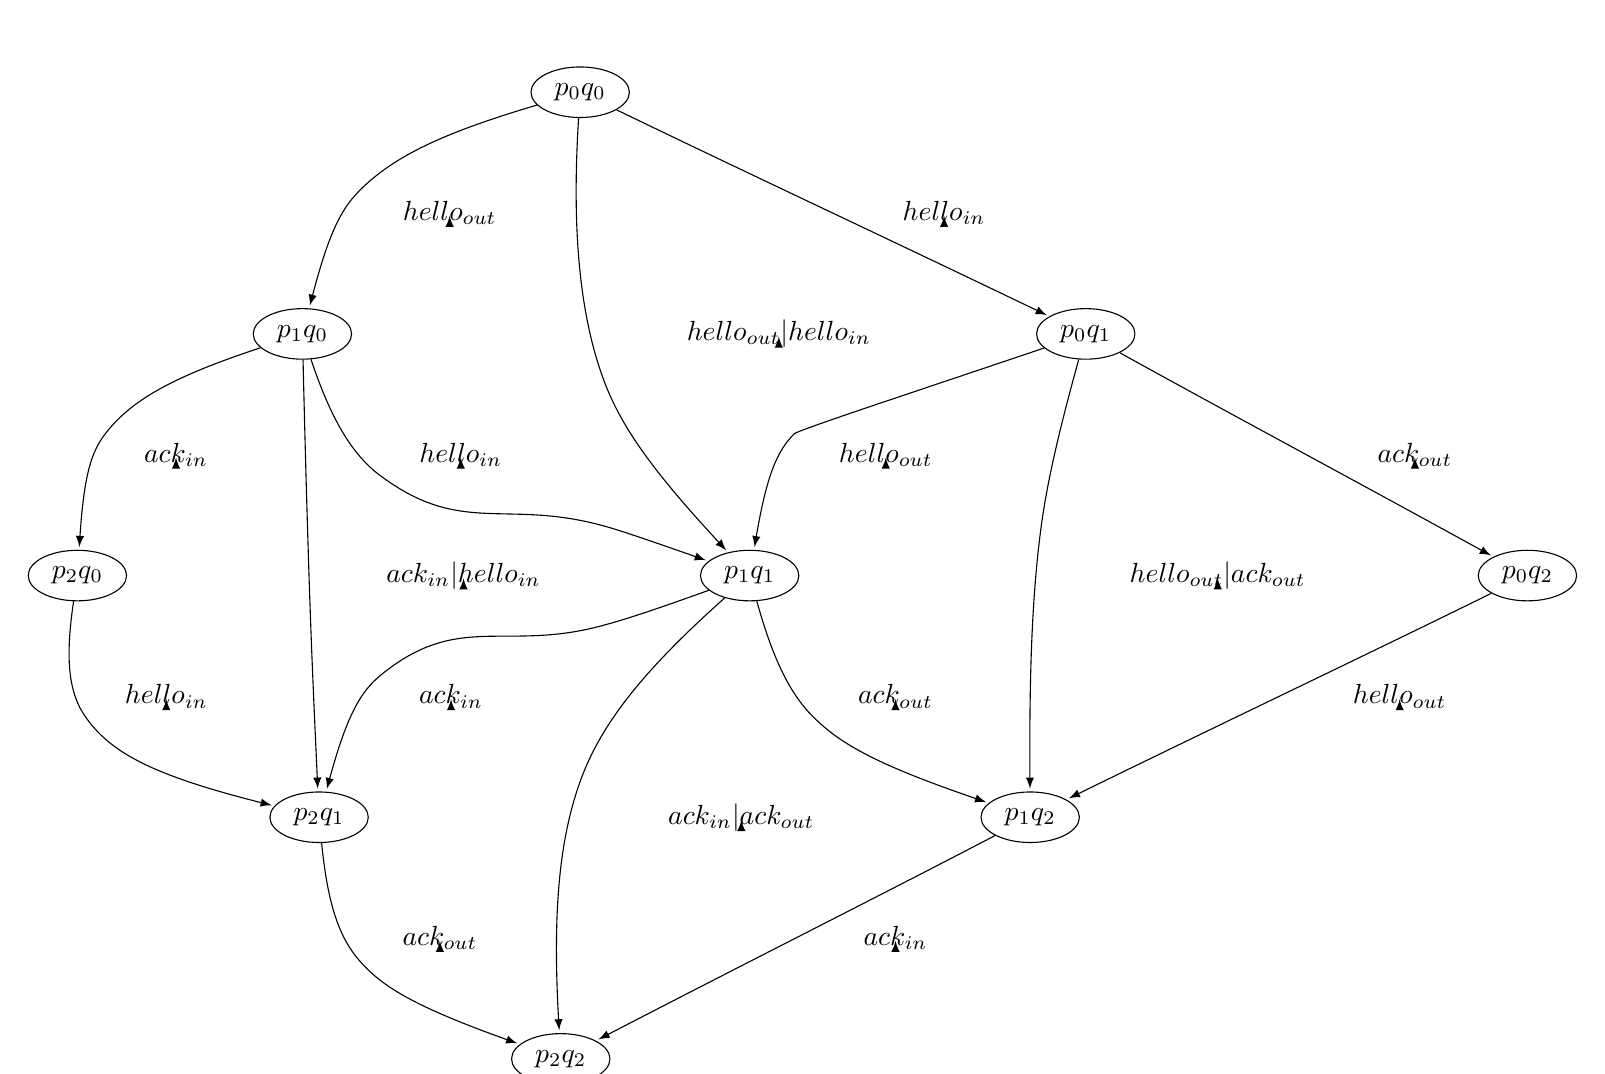
\begin{tikzpicture}[>=latex,line join=bevel,]
%%
\begin{scope}
  \pgfsetstrokecolor{black}
  \definecolor{strokecol}{rgb}{1.0,1.0,1.0};
  \pgfsetstrokecolor{strokecol}
  \definecolor{fillcol}{rgb}{1.0,1.0,1.0};
  \pgfsetfillcolor{fillcol}
\end{scope}
\begin{scope}
  \pgfsetstrokecolor{black}
  \definecolor{strokecol}{rgb}{1.0,1.0,1.0};
  \pgfsetstrokecolor{strokecol}
  \definecolor{fillcol}{rgb}{1.0,1.0,1.0};
  \pgfsetfillcolor{fillcol}
\end{scope}
\begin{scope}
  \pgfsetstrokecolor{black}
  \definecolor{strokecol}{rgb}{1.0,1.0,1.0};
  \pgfsetstrokecolor{strokecol}
  \definecolor{fillcol}{rgb}{1.0,1.0,1.0};
  \pgfsetfillcolor{fillcol}
\end{scope}
\begin{scope}
  \pgfsetstrokecolor{black}
  \definecolor{strokecol}{rgb}{1.0,1.0,1.0};
  \pgfsetstrokecolor{strokecol}
  \definecolor{fillcol}{rgb}{1.0,1.0,1.0};
  \pgfsetfillcolor{fillcol}
\end{scope}
  \node (p_1q_2) at (382.0bp,105.0bp) [draw,ellipse] {$p_1q_2$};
  \node (p_2q_1) at (126.0bp,105.0bp) [draw,ellipse] {$p_2q_1$};
  \node (p_1q_0) at (120.0bp,279.0bp) [draw,ellipse] {$p_1q_0$};
  \node (p_2q_0) at (38.997bp,192.0bp) [draw,ellipse] {$p_2q_0$};
  \node (p_1q_1) at (281.0bp,192.0bp) [draw,ellipse] {$p_1q_1$};
  \node (p_0q_1) at (402.0bp,279.0bp) [draw,ellipse] {$p_0q_1$};
  \node (p_0q_0) at (220.0bp,366.0bp) [draw,ellipse] {$p_0q_0$};
  \node (p_0q_2) at (561.0bp,192.0bp) [draw,ellipse] {$p_0q_2$};
  \node (p_2q_2) at (213.0bp,18.0bp) [draw,ellipse] {$p_2q_2$};
  \draw [->] (p_2q_1) ..controls (128.86bp,76.122bp) and (132.35bp,63.113bp)  .. (140.0bp,54.0bp) .. controls (148.12bp,44.329bp) and (159.53bp,37.135bp)  .. (p_2q_2);
  \definecolor{strokecol}{rgb}{0.0,0.0,0.0};
  \pgfsetstrokecolor{strokecol}
  \draw (169.5bp,61.5bp) node {$ack_{out}$};
  \draw [->] (p_1q_0) ..controls (129.71bp,250.1bp) and (136.99bp,236.21bp)  .. (148.0bp,228.0bp) .. controls (177.21bp,206.21bp) and (192.83bp,219.58bp)  .. (228.0bp,210.0bp) .. controls (232.09bp,208.89bp) and (236.33bp,207.65bp)  .. (p_1q_1);
  \draw (177.0bp,235.5bp) node {$hello_{in}$};
  \draw [->] (p_1q_0) ..controls (120.93bp,240.06bp) and (121.88bp,204.51bp)  .. (123.0bp,174.0bp) .. controls (123.49bp,160.57bp) and (124.13bp,145.66bp)  .. (p_2q_1);
  \draw (178.0bp,192.0bp) node {$ack_{in}|hello_{in}$};
  \draw [->] (p_1q_2) ..controls (327.7bp,76.69bp) and (280.01bp,52.704bp)  .. (p_2q_2);
  \draw (333.5bp,61.5bp) node {$ack_{in}$};
  \draw [->] (p_1q_1) ..controls (243.03bp,178.33bp) and (235.27bp,175.98bp)  .. (228.0bp,174.0bp) .. controls (192.83bp,164.42bp) and (176.13bp,179.16bp)  .. (148.0bp,156.0bp) .. controls (140.84bp,150.11bp) and (135.94bp,141.43bp)  .. (p_2q_1);
  \draw (173.5bp,148.5bp) node {$ack_{in}$};
  \draw [->] (p_0q_0) ..controls (217.55bp,326.59bp) and (217.8bp,289.9bp)  .. (229.0bp,261.0bp) .. controls (235.43bp,244.4bp) and (247.22bp,228.45bp)  .. (p_1q_1);
  \draw (291.5bp,279.0bp) node {$hello_{out}|hello_{in}$};
  \draw [->] (p_0q_2) ..controls (503.56bp,163.73bp) and (451.96bp,139.22bp)  .. (p_1q_2);
  \draw (515.0bp,148.5bp) node {$hello_{out}$};
  \draw [->] (p_1q_1) ..controls (289.03bp,163.29bp) and (294.9bp,150.01bp)  .. (304.0bp,141.0bp) .. controls (313.91bp,131.18bp) and (327.07bp,123.85bp)  .. (p_1q_2);
  \draw (333.5bp,148.5bp) node {$ack_{out}$};
  \draw [->] (p_1q_1) ..controls (249.08bp,163.44bp) and (230.95bp,144.16bp)  .. (222.0bp,123.0bp) .. controls (211.66bp,98.586bp) and (210.2bp,68.115bp)  .. (p_2q_2);
  \draw (278.0bp,105.0bp) node {$ack_{in}|ack_{out}$};
  \draw [->] (p_2q_0) ..controls (34.756bp,163.36bp) and (35.346bp,150.36bp)  .. (41.997bp,141.0bp) .. controls (50.995bp,128.34bp) and (65.471bp,120.24bp)  .. (p_2q_1);
  \draw (70.997bp,148.5bp) node {$hello_{in}$};
  \draw [->] (p_0q_0) ..controls (170.41bp,351.29bp) and (152.44bp,342.85bp)  .. (140.0bp,330.0bp) .. controls (133.8bp,323.6bp) and (129.45bp,315.04bp)  .. (p_1q_0);
  \draw (173.0bp,322.5bp) node {$hello_{out}$};
  \draw [->] (p_0q_0) ..controls (278.0bp,337.91bp) and (330.85bp,313.23bp)  .. (p_0q_1);
  \draw (351.0bp,322.5bp) node {$hello_{in}$};
  \draw [->] (p_0q_1) ..controls (393.31bp,247.47bp) and (388.39bp,227.67bp)  .. (386.0bp,210.0bp) .. controls (382.48bp,184.08bp) and (381.66bp,154.22bp)  .. (p_1q_2);
  \draw (449.5bp,192.0bp) node {$hello_{out}|ack_{out}$};
  \draw [->] (p_0q_1) ..controls (453.57bp,250.43bp) and (497.35bp,227.03bp)  .. (p_0q_2);
  \draw (520.5bp,235.5bp) node {$ack_{out}$};
  \draw [->] (p_0q_1) ..controls (340.56bp,258.2bp) and (298.37bp,244.39bp)  .. (297.0bp,243.0bp) .. controls (290.96bp,236.89bp) and (287.2bp,228.51bp)  .. (p_1q_1);
  \draw (330.0bp,235.5bp) node {$hello_{out}$};
  \draw [->] (p_1q_0) ..controls (73.4bp,263.58bp) and (58.458bp,255.31bp)  .. (48.997bp,243.0bp) .. controls (44.047bp,236.56bp) and (41.361bp,228.31bp)  .. (p_2q_0);
  \draw (74.497bp,235.5bp) node {$ack_{in}$};
%
\end{tikzpicture}

	\caption{LTS of $ P \Vert Q $} \label{fig:CommunicationOperatorProcess}
	\endminipage\hfill
	\minipage{0.33\textwidth}
	\centering
	
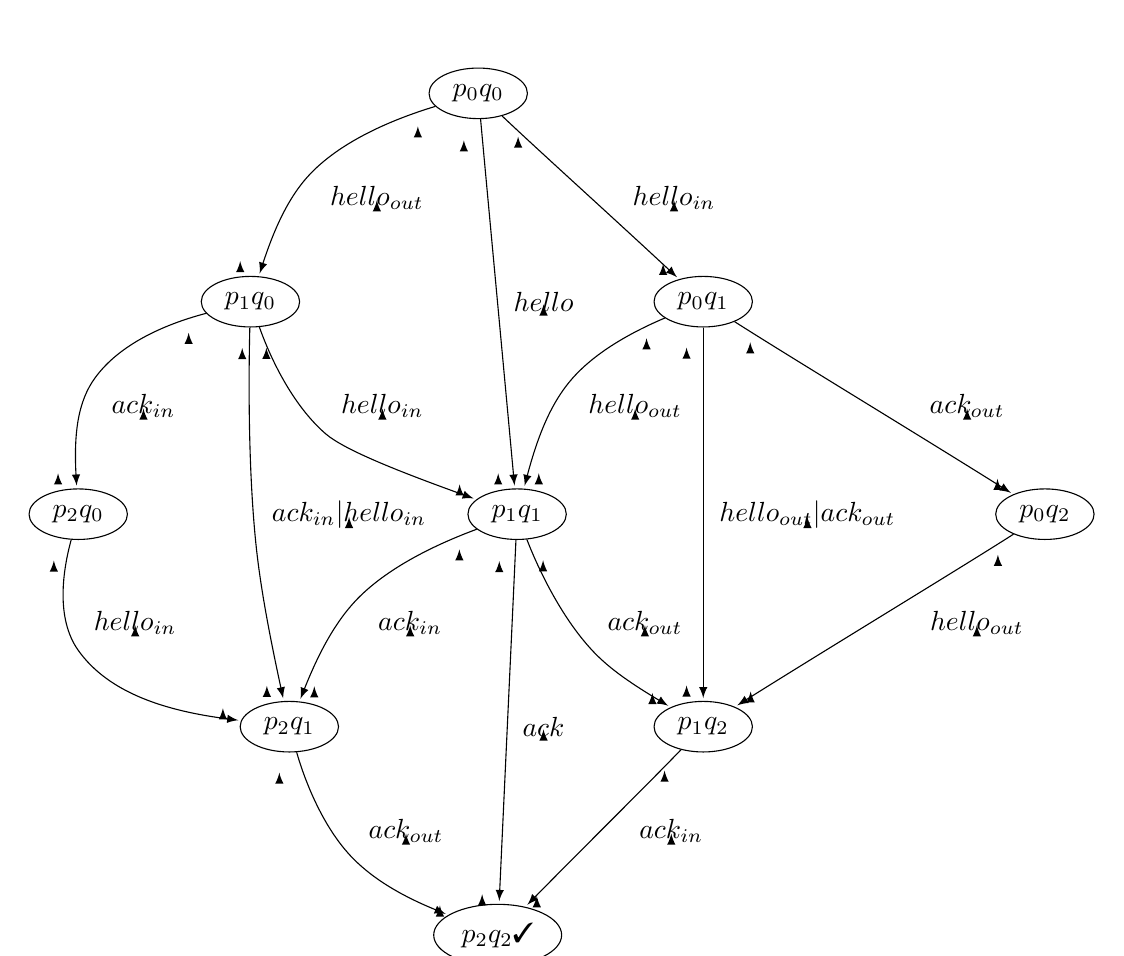
\begin{tikzpicture}[>=latex,line join=bevel,]
%%
\begin{scope}
  \pgfsetstrokecolor{black}
  \definecolor{strokecol}{rgb}{1.0,1.0,1.0};
  \pgfsetstrokecolor{strokecol}
  \definecolor{fillcol}{rgb}{1.0,1.0,1.0};
  \pgfsetfillcolor{fillcol}
  \filldraw (0.0bp,0.0bp) -- (0.0bp,322.0bp) -- (384.0bp,322.0bp) -- (384.0bp,0.0bp) -- cycle;
\end{scope}
\begin{scope}
  \pgfsetstrokecolor{black}
  \definecolor{strokecol}{rgb}{1.0,1.0,1.0};
  \pgfsetstrokecolor{strokecol}
  \definecolor{fillcol}{rgb}{1.0,1.0,1.0};
  \pgfsetfillcolor{fillcol}
  \filldraw (0.0bp,0.0bp) -- (0.0bp,322.0bp) -- (384.0bp,322.0bp) -- (384.0bp,0.0bp) -- cycle;
\end{scope}
\begin{scope}
  \pgfsetstrokecolor{black}
  \definecolor{strokecol}{rgb}{1.0,1.0,1.0};
  \pgfsetstrokecolor{strokecol}
  \definecolor{fillcol}{rgb}{1.0,1.0,1.0};
  \pgfsetfillcolor{fillcol}
  \filldraw (0.0bp,0.0bp) -- (0.0bp,322.0bp) -- (384.0bp,322.0bp) -- (384.0bp,0.0bp) -- cycle;
\end{scope}
\begin{scope}
  \pgfsetstrokecolor{black}
  \definecolor{strokecol}{rgb}{1.0,1.0,1.0};
  \pgfsetstrokecolor{strokecol}
  \definecolor{fillcol}{rgb}{1.0,1.0,1.0};
  \pgfsetfillcolor{fillcol}
  \filldraw (0.0bp,0.0bp) -- (0.0bp,322.0bp) -- (384.0bp,322.0bp) -- (384.0bp,0.0bp) -- cycle;
\end{scope}
  \node (p_1q_2) at (243.0bp,84.5bp) [draw,ellipse] {$p_1q_2$};
  \node (p_2q_1) at (94.0bp,84.5bp) [draw,ellipse] {$p_2q_1$};
  \node (p_1q_0) at (80.0bp,237.5bp) [draw,ellipse] {$p_1q_0$};
  \node (p_2q_0) at (18.0bp,161.0bp) [draw,ellipse] {$p_2q_0$};
  \node (p_1q_1) at (176.0bp,161.0bp) [draw,ellipse] {$p_1q_1$};
  \node (p_0q_1) at (243.0bp,237.5bp) [draw,ellipse] {$p_0q_1$};
  \node (p_0q_0) at (162.0bp,312.5bp) [draw,ellipse] {$p_0q_0$};
  \node (p_0q_2) at (366.0bp,161.0bp) [draw,ellipse] {$p_0q_2$};
  \node (p_2q_2) at (169.0bp,9.5bp) [draw,ellipse] {$p_2q_2 \text{\cmark}$};
  \draw [->] (p_2q_1) ..controls (99.627bp,64.823bp) and (106.24bp,47.891bp)  .. (117.0bp,37.0bp) .. controls (124.72bp,29.19bp) and (135.22bp,23.244bp)  .. (p_2q_2);
  \definecolor{strokecol}{rgb}{0.0,0.0,0.0};
  \pgfsetstrokecolor{strokecol}
  \draw (136.0bp,47.0bp) node {$ack_{out}$};
  \draw (90.4bp,68.97bp) node {$$};
  \draw (148.21bp,21.145bp) node {$$};
  \draw [->] (p_1q_0) ..controls (87.043bp,217.5bp) and (95.018bp,200.41bp)  .. (107.0bp,190.0bp) .. controls (113.95bp,183.96bp) and (134.53bp,175.98bp)  .. (p_1q_1);
  \draw (127.5bp,200.0bp) node {$hello_{in}$};
  \draw (77.037bp,221.81bp) node {$$};
  \draw (155.3bp,172.71bp) node {$$};
  \draw [->] (p_1q_0) ..controls (79.377bp,212.29bp) and (79.05bp,178.39bp)  .. (82.0bp,150.0bp) .. controls (83.621bp,134.4bp) and (86.969bp,116.93bp)  .. (p_2q_1);
  \draw (115.5bp,161.0bp) node {$ack_{in}|hello_{in}$};
  \draw (85.742bp,221.88bp) node {$$};
  \draw (85.92bp,100.2bp) node {$$};
  \draw [->] (p_1q_2) ..controls (223.02bp,63.786bp) and (199.81bp,40.889bp)  .. (p_2q_2);
  \draw (231.5bp,47.0bp) node {$ack_{in}$};
  \draw (229.08bp,69.688bp) node {$$};
  \draw (183.09bp,24.477bp) node {$$};
  \draw [->] (p_1q_1) ..controls (148.99bp,150.94bp) and (131.79bp,143.26bp)  .. (120.0bp,132.0bp) .. controls (111.65bp,124.03bp) and (105.26bp,112.77bp)  .. (p_2q_1);
  \draw (137.5bp,122.0bp) node {$ack_{in}$};
  \draw (155.21bp,149.37bp) node {$$};
  \draw (102.98bp,100.04bp) node {$$};
  \draw [->] (p_0q_0) ..controls (165.07bp,278.75bp) and (171.22bp,213.08bp)  .. (p_1q_1);
  \draw (185.5bp,237.5bp) node {$hello$};
  \draw (156.83bp,296.6bp) node {$$};
  \draw (169.19bp,176.67bp) node {$$};
  \draw [->] (p_0q_2) ..controls (334.35bp,140.83bp) and (289.0bp,113.36bp)  .. (p_1q_2);
  \draw (341.5bp,122.0bp) node {$hello_{out}$};
  \draw (349.08bp,147.39bp) node {$$};
  \draw (260.07bp,98.204bp) node {$$};
  \draw [->] (p_1q_1) ..controls (183.66bp,141.16bp) and (191.93bp,123.9bp)  .. (203.0bp,112.0bp) .. controls (208.34bp,106.26bp) and (215.15bp,101.16bp)  .. (p_1q_2);
  \draw (222.0bp,122.0bp) node {$ack_{out}$};
  \draw (185.35bp,145.42bp) node {$$};
  \draw (224.7bp,97.631bp) node {$$};
  \draw [->] (p_1q_1) ..controls (174.47bp,127.36bp) and (171.42bp,62.155bp)  .. (p_2q_2);
  \draw (185.5bp,84.5bp) node {$ack$};
  \draw (169.58bp,145.1bp) node {$$};
  \draw (163.41bp,25.17bp) node {$$};
  \draw [->] (p_2q_0) ..controls (12.488bp,140.93bp) and (9.7958bp,123.55bp)  .. (18.0bp,112.0bp) .. controls (28.856bp,96.717bp) and (49.206bp,90.175bp)  .. (p_2q_1);
  \draw (38.5bp,122.0bp) node {$hello_{in}$};
  \draw (9.2224bp,145.3bp) node {$$};
  \draw (70.087bp,92.13bp) node {$$};
  \draw [->] (p_0q_0) ..controls (133.3bp,303.78bp) and (115.13bp,296.69bp)  .. (103.0bp,285.0bp) .. controls (94.989bp,277.28bp) and (89.354bp,266.19bp)  .. (p_1q_0);
  \draw (125.5bp,275.0bp) node {$hello_{out}$};
  \draw (140.27bp,301.64bp) node {$$};
  \draw (76.31bp,253.12bp) node {$$};
  \draw [->] (p_0q_0) ..controls (183.7bp,291.94bp) and (210.02bp,268.22bp)  .. (p_0q_1);
  \draw (232.5bp,275.0bp) node {$hello_{in}$};
  \draw (176.36bp,297.96bp) node {$$};
  \draw (228.56bp,252.11bp) node {$$};
  \draw [->] (p_0q_1) ..controls (243.0bp,204.29bp) and (243.0bp,137.51bp)  .. (p_1q_2);
  \draw (280.5bp,161.0bp) node {$hello_{out}|ack_{out}$};
  \draw (237.0bp,221.95bp) node {$$};
  \draw (237.0bp,100.33bp) node {$$};
  \draw [->] (p_0q_1) ..controls (274.65bp,217.33bp) and (320.0bp,189.86bp)  .. (p_0q_2);
  \draw (338.0bp,200.0bp) node {$ack_{out}$};
  \draw (259.92bp,223.89bp) node {$$};
  \draw (348.93bp,174.7bp) node {$$};
  \draw [->] (p_0q_1) ..controls (218.33bp,227.01bp) and (204.83bp,219.95bp)  .. (196.0bp,210.0bp) .. controls (188.6bp,201.66bp) and (183.68bp,190.2bp)  .. (p_1q_1);
  \draw (218.5bp,200.0bp) node {$hello_{out}$};
  \draw (222.59bp,225.33bp) node {$$};
  \draw (183.8bp,176.73bp) node {$$};
  \draw [->] (p_1q_0) ..controls (50.826bp,229.83bp) and (33.397bp,222.98bp)  .. (24.0bp,210.0bp) .. controls (17.983bp,201.69bp) and (16.343bp,190.38bp)  .. (p_2q_0);
  \draw (41.5bp,200.0bp) node {$ack_{in}$};
  \draw (57.754bp,227.29bp) node {$$};
  \draw (10.742bp,176.7bp) node {$$};
%
\end{tikzpicture}

	\caption{LTS of $\Gamma_{\{hello_{in} | hello_{out} \rightarrow hello, ack_{in} | ack_{out} \rightarrow ack\}}(P \Vert Q) $} \label{fig:CommunicationOperatorCommunicate}
	\endminipage\hfill
	\minipage{0.33\textwidth}
	\centering
	
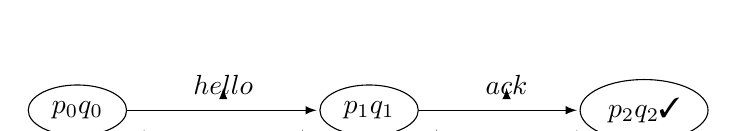
\begin{tikzpicture}[>=latex,line join=bevel,]
%%
\node (p_0q_0) at (18.0bp,12.0bp) [draw,ellipse] {$p_0q_0$};
  \node (p_2q_2) at (222.0bp,12.0bp) [draw,ellipse] {$p_2q_2 \text{\cmark}$};
  \node (p_1q_1) at (123.0bp,12.0bp) [draw,ellipse] {$p_1q_1$};
  \draw [->] (p_1q_1) ..controls (155.82bp,12.0bp) and (176.74bp,12.0bp)  .. (p_2q_2);
  \definecolor{strokecol}{rgb}{0.0,0.0,0.0};
  \pgfsetstrokecolor{strokecol}
  \draw (172.5bp,21.0bp) node {$ack$};
  \draw (147.34bp,6.0bp) node {$$};
  \draw (197.81bp,6.0bp) node {$$};
  \draw [->] (p_0q_0) ..controls (51.962bp,12.0bp) and (76.087bp,12.0bp)  .. (p_1q_1);
  \draw (70.5bp,21.0bp) node {$hello$};
  \draw (42.008bp,6.0bp) node {$$};
  \draw (98.966bp,6.0bp) node {$$};
%
\end{tikzpicture}

	\caption{LTS of $ \nabla_{\{hello, ack\}}\Gamma_{\{hello_{in} | hello_{out} \rightarrow hello, ack_{in} | ack_{out} \rightarrow ack\}}(P \Vert Q) $} \label{fig:CommunicationOperatorAllow}
	\endminipage\hfill
\end{figure}

\subsection{Axioms of the Process Algebras}

We indicated previously in this section the need for formal axioms for the process algebra in order to be able to operate on it. These axioms vary from simple, lengthy, straightforward and convoluted, and unfortunately must be left out of this work. To consult these axioms, please read Chapter 1, Sections 4 and 5 of \cite{Groote:2014:MAC:2628007}.

\section{Process Equivalence}
The most basic task one must be interested in when modeling and verifying processes is knowing if two processes are equivalent. In this sections I will present the different equivalences commonly used, their properties and when to use them.
\subsection{Equivalences without internal actions}
We will show here the following equivalences, intended for verifying properties that involve knowing all actions performed by the system.
\subsubsection{Trace equivalence} 
The trace equivalence is the loosest of the equivalences usually used, that is, any processes that are equivalent by other definitions must be also trace equivalent, but not the converse. We can see trace equivalence as the equivalence of the sequences of actions possible from the initial states. This equivalence does not analyze communication between actions, and therefore we cannot ''identify´´ deadlocks. Each trace, is represented by the concatenation of the actions executed along. We also include the finishing symbol when we reach a terminating state so that no new action can be performed.
\begin{definition} [Trace equivalence]
	Let $ A = (S, Act, \rightarrow, s_0, T) $ be a LTS. The set of traces starting from $ t \in S$, $ Traces(t) $, is the minimal set that satisfies:
	\begin{itemize}
		\item $ \varepsilon \in Traces(t) $
		\item \cmark $ \in Traces(t) \iff t \in T $
		\item $ t\xrightarrow{a} t’ \wedge \sigma \in Traces(t’) \Rightarrow a\cdot\sigma \in Traces(t) $
	\end{itemize}
\end{definition}

As we said previously, when we simply talk about the set of traces of an LTS we are referring to the one starting from the initial state of the LTS, $ Traces(s_0) $. Now, two states are trace equivalent if their set of traces are equal, and two LTS are equivalent if their initial states are so. 

The trace equivalence is to be used when the sequence of actions is the only thing we are interested in, without preserving any branching behavior. In this case, trace equivalence is the best suited, as it can reduce LTS to some smaller equivalent LTS, than the other equivalences.
We must also consider the fact that computing the trace of an arbitrary LTS is not at all efficient. To be precise, to decide trace equivalence is a $ PSPACE-Complete $ problem \cite{KANELLAKIS199043}.

An example of two trace equivalent processes is given by processes $ P = (a·c) + (b·c) $ and $ Q = (a + b)·c $. Their LTS's are:

\begin{figure} [H]
	\minipage{0.5\textwidth}
	\centering
	
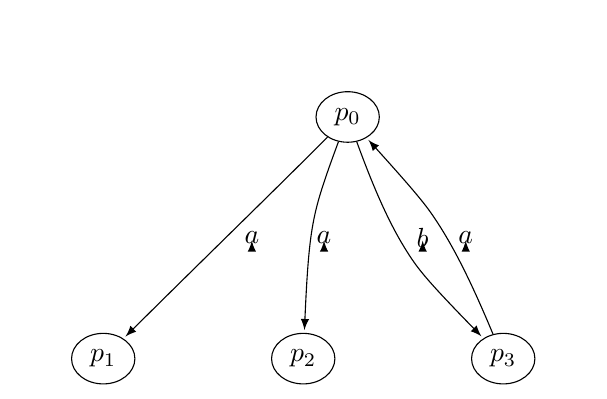
\begin{tikzpicture}[>=latex,line join=bevel,]
%%
\begin{scope}
  \pgfsetstrokecolor{black}
  \definecolor{strokecol}{rgb}{1.0,1.0,1.0};
  \pgfsetstrokecolor{strokecol}
  \definecolor{fillcol}{rgb}{1.0,1.0,1.0};
  \pgfsetfillcolor{fillcol}
  \filldraw (0.0bp,0.0bp) -- (0.0bp,123.0bp) -- (198.0bp,123.0bp) -- (198.0bp,0.0bp) -- cycle;
\end{scope}
  \node (p_2) at (99.0bp,18.0bp) [draw,ellipse] {$p_2$};
  \node (p_3) at (171.0bp,18.0bp) [draw,ellipse] {$p_3$};
  \node (p_0) at (115.0bp,105.0bp) [draw,ellipse] {$p_0$};
  \node (p_1) at (27.0bp,18.0bp) [draw,ellipse] {$p_1$};
  \draw [->] (p_3) ..controls (159.4bp,45.816bp) and (153.06bp,58.546bp)  .. (146.0bp,69.0bp) .. controls (143.06bp,73.344bp) and (139.64bp,77.725bp)  .. (p_0);
  \definecolor{strokecol}{rgb}{0.0,0.0,0.0};
  \pgfsetstrokecolor{strokecol}
  \draw (157.5bp,61.5bp) node {$a$};
  \draw [->] (p_0) ..controls (106.34bp,81.737bp) and (104.28bp,75.163bp)  .. (103.0bp,69.0bp) .. controls (101.48bp,61.698bp) and (100.53bp,53.686bp)  .. (p_2);
  \draw (106.5bp,61.5bp) node {$a$};
  \draw [->] (p_0) ..controls (86.081bp,76.067bp) and (64.992bp,55.697bp)  .. (p_1);
  \draw (80.5bp,61.5bp) node {$a$};
  \draw [->] (p_0) ..controls (125.23bp,77.03bp) and (131.05bp,64.297bp)  .. (138.0bp,54.0bp) .. controls (141.15bp,49.327bp) and (144.94bp,44.685bp)  .. (p_3);
  \draw (142.0bp,61.5bp) node {$b$};
%
\end{tikzpicture}

	\caption{LTS of $P$} \label{fig:TraceEquivalenceP}
	\endminipage\hfill
	\minipage{0.5\textwidth}
	\centering
	
\begin{tikzpicture}[>=latex,line join=bevel,]
%%
\node (q_7) at (99.0bp,18.0bp) [draw,ellipse] {$q_7$};
  \node (q_6) at (243.0bp,105.0bp) [draw,ellipse] {$q_6$};
  \node (q_5) at (171.0bp,105.0bp) [draw,ellipse] {$q_5$};
  \node (q_4) at (99.0bp,105.0bp) [draw,ellipse] {$q_4$};
  \node (q_3) at (27.0bp,105.0bp) [draw,ellipse] {$q_3$};
  \node (q_2) at (171.0bp,192.0bp) [draw,ellipse] {$q_2$};
  \node (q_1) at (99.0bp,192.0bp) [draw,ellipse] {$q_1$};
  \node (q_0) at (140.0bp,279.0bp) [draw,ellipse] {$q_0$};
  \node (q_8) at (171.0bp,18.0bp) [draw,ellipse] {$q_8$};
  \draw [->] (q_1) ..controls (75.07bp,162.75bp) and (58.964bp,143.74bp)  .. (q_3);
  \definecolor{strokecol}{rgb}{0.0,0.0,0.0};
  \pgfsetstrokecolor{strokecol}
  \draw (72.0bp,148.5bp) node {$b$};
  \draw [->] (q_4) ..controls (99.0bp,75.163bp) and (99.0bp,59.548bp)  .. (q_7);
  \draw (102.5bp,61.5bp) node {$e$};
  \draw [->] (q_0) ..controls (126.2bp,249.38bp) and (118.03bp,232.44bp)  .. (q_1);
  \draw (125.5bp,235.5bp) node {$a$};
  \draw [->] (q_1) ..controls (99.0bp,162.16bp) and (99.0bp,146.55bp)  .. (q_4);
  \draw (102.5bp,148.5bp) node {$c$};
  \draw [->] (q_0) ..controls (150.5bp,249.22bp) and (156.47bp,232.85bp)  .. (q_2);
  \draw (161.5bp,235.5bp) node {$a$};
  \draw [->] (q_5) ..controls (171.0bp,75.163bp) and (171.0bp,59.548bp)  .. (q_8);
  \draw (175.0bp,61.5bp) node {$d$};
  \draw [->] (q_2) ..controls (194.93bp,162.75bp) and (211.04bp,143.74bp)  .. (q_6);
  \draw (214.5bp,148.5bp) node {$f$};
  \draw [->] (q_2) ..controls (171.0bp,162.16bp) and (171.0bp,146.55bp)  .. (q_5);
  \draw (174.5bp,148.5bp) node {$c$};
%
\end{tikzpicture}

	\caption{LTS of $Q$} \label{fig:TraceEquivalenceQ}
	\endminipage\hfill
\end{figure}

It is obvious that both LTS's have as set of traces $ \{ \epsilon,a,b,a·c,b·c,a·c·$\cmark$,b·c·$\cmark$\} $ and therefore they are trace equivalent.

\subsubsection{Completed trace equivalence} 
Completed trace equivalence differs from trace equivalence in that it only includes sequences of actions that end in a terminating state or in a deadlock.
\begin{definition} [Completed trace equivalence]
	Let $ A = (S, Act, \rightarrow, s_0, T) $ be a LTS. The set of completed traces starting from $ t \in S $, $ CompletedTraces(t) $, is the minimal set that satisfies:
	\begin{itemize}
		\item $ \varepsilon \in CompletedTraces(t) $ if $ t \not \in T \wedge \not \exists t\xrightarrow{a}t’$
		\item \cmark $\in CompletedTraces(t) \iff t \in T$
		\item $ t\xrightarrow{a}t’ \wedge \sigma \in CompletedTraces(t’) \Rightarrow a\cdot\sigma \in CompletedTraces(t)$
	\end{itemize}
\end{definition}
We can observe that the only difference between the definition of Traces(t) and CompletedTraces(t) is that we do not include the empty sequence by default, thus not generating all partial sequences previous to reaching a terminating or deadlocked state.
As a consequence we can build on top of traces equivalence a certain detection of deadlocks. The drawback of this is that it is not preserved by all the defined operators. Namely, the blocking operator applied to two complete trace equivalent LTSs can make the resulting LTSs not equivalent. This an inmediate consequence of the fact that whenever any state of an LTS has some transition leaving it, we have CompletedTraces(t) = $ \emptyset \forall t \in S$.

In particular, for $ P = a·b·P + a·c·P $ and $ Q = a·(b+c)·P $, we have that both generate infinite sequences of a's interleaved with b's and c's. Because these sequences are infinite, complete trace sets for both processes are empty, and therefore both processes are complete trace equivalent.

\begin{figure} [H]
	\minipage{0.5\textwidth}
	\centering
	
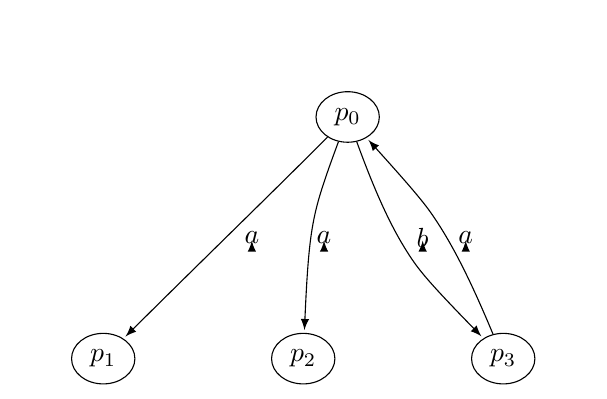
\begin{tikzpicture}[>=latex,line join=bevel,]
%%
\begin{scope}
  \pgfsetstrokecolor{black}
  \definecolor{strokecol}{rgb}{1.0,1.0,1.0};
  \pgfsetstrokecolor{strokecol}
  \definecolor{fillcol}{rgb}{1.0,1.0,1.0};
  \pgfsetfillcolor{fillcol}
  \filldraw (0.0bp,0.0bp) -- (0.0bp,123.0bp) -- (198.0bp,123.0bp) -- (198.0bp,0.0bp) -- cycle;
\end{scope}
  \node (p_2) at (99.0bp,18.0bp) [draw,ellipse] {$p_2$};
  \node (p_3) at (171.0bp,18.0bp) [draw,ellipse] {$p_3$};
  \node (p_0) at (115.0bp,105.0bp) [draw,ellipse] {$p_0$};
  \node (p_1) at (27.0bp,18.0bp) [draw,ellipse] {$p_1$};
  \draw [->] (p_3) ..controls (159.4bp,45.816bp) and (153.06bp,58.546bp)  .. (146.0bp,69.0bp) .. controls (143.06bp,73.344bp) and (139.64bp,77.725bp)  .. (p_0);
  \definecolor{strokecol}{rgb}{0.0,0.0,0.0};
  \pgfsetstrokecolor{strokecol}
  \draw (157.5bp,61.5bp) node {$a$};
  \draw [->] (p_0) ..controls (106.34bp,81.737bp) and (104.28bp,75.163bp)  .. (103.0bp,69.0bp) .. controls (101.48bp,61.698bp) and (100.53bp,53.686bp)  .. (p_2);
  \draw (106.5bp,61.5bp) node {$a$};
  \draw [->] (p_0) ..controls (86.081bp,76.067bp) and (64.992bp,55.697bp)  .. (p_1);
  \draw (80.5bp,61.5bp) node {$a$};
  \draw [->] (p_0) ..controls (125.23bp,77.03bp) and (131.05bp,64.297bp)  .. (138.0bp,54.0bp) .. controls (141.15bp,49.327bp) and (144.94bp,44.685bp)  .. (p_3);
  \draw (142.0bp,61.5bp) node {$b$};
%
\end{tikzpicture}

	\caption{LTS of $P$} \label{fig:CompleteTraceEquivalenceP}
	\endminipage\hfill
	\minipage{0.5\textwidth}
	\centering
	
\begin{tikzpicture}[>=latex,line join=bevel,]
%%
\node (q_7) at (99.0bp,18.0bp) [draw,ellipse] {$q_7$};
  \node (q_6) at (243.0bp,105.0bp) [draw,ellipse] {$q_6$};
  \node (q_5) at (171.0bp,105.0bp) [draw,ellipse] {$q_5$};
  \node (q_4) at (99.0bp,105.0bp) [draw,ellipse] {$q_4$};
  \node (q_3) at (27.0bp,105.0bp) [draw,ellipse] {$q_3$};
  \node (q_2) at (171.0bp,192.0bp) [draw,ellipse] {$q_2$};
  \node (q_1) at (99.0bp,192.0bp) [draw,ellipse] {$q_1$};
  \node (q_0) at (140.0bp,279.0bp) [draw,ellipse] {$q_0$};
  \node (q_8) at (171.0bp,18.0bp) [draw,ellipse] {$q_8$};
  \draw [->] (q_1) ..controls (75.07bp,162.75bp) and (58.964bp,143.74bp)  .. (q_3);
  \definecolor{strokecol}{rgb}{0.0,0.0,0.0};
  \pgfsetstrokecolor{strokecol}
  \draw (72.0bp,148.5bp) node {$b$};
  \draw [->] (q_4) ..controls (99.0bp,75.163bp) and (99.0bp,59.548bp)  .. (q_7);
  \draw (102.5bp,61.5bp) node {$e$};
  \draw [->] (q_0) ..controls (126.2bp,249.38bp) and (118.03bp,232.44bp)  .. (q_1);
  \draw (125.5bp,235.5bp) node {$a$};
  \draw [->] (q_1) ..controls (99.0bp,162.16bp) and (99.0bp,146.55bp)  .. (q_4);
  \draw (102.5bp,148.5bp) node {$c$};
  \draw [->] (q_0) ..controls (150.5bp,249.22bp) and (156.47bp,232.85bp)  .. (q_2);
  \draw (161.5bp,235.5bp) node {$a$};
  \draw [->] (q_5) ..controls (171.0bp,75.163bp) and (171.0bp,59.548bp)  .. (q_8);
  \draw (175.0bp,61.5bp) node {$d$};
  \draw [->] (q_2) ..controls (194.93bp,162.75bp) and (211.04bp,143.74bp)  .. (q_6);
  \draw (214.5bp,148.5bp) node {$f$};
  \draw [->] (q_2) ..controls (171.0bp,162.16bp) and (171.0bp,146.55bp)  .. (q_5);
  \draw (174.5bp,148.5bp) node {$c$};
%
\end{tikzpicture}

	\caption{LTS of $Q$} \label{fig:CompleteTraceEquivalenceQ}
	\endminipage\hfill
\end{figure}

But when the blocking operator of action c is applied to P and Q, the resulting processes become not complete trace equivalent, as we can easily see in the generated LTS's: the first, corresponding to P, has $ a·\cmark $ as a complete trace, which is not the case when blocking Q.

\begin{figure} [H]
	\minipage{0.5\textwidth}
	\centering
	
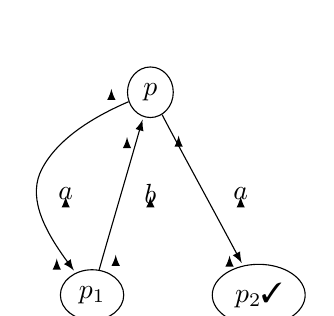
\begin{tikzpicture}[>=latex,line join=bevel,]
%%
\node (p) at (41.284bp,82.5bp) [draw,ellipse] {$p$};
  \node (p_2) at (80.284bp,9.5bp) [draw,ellipse] {$p_2\text{\cmark}$};
  \node (p_1) at (20.284bp,9.5bp) [draw,ellipse] {$p_1$};
  \draw [->] (p_1) ..controls (26.041bp,29.966bp) and (31.78bp,49.367bp)  .. (p);
  \definecolor{strokecol}{rgb}{0.0,0.0,0.0};
  \pgfsetstrokecolor{strokecol}
  \draw (41.284bp,46.0bp) node {$b$};
  \draw (28.795bp,24.989bp) node {$$};
  \draw (32.875bp,67.355bp) node {$$};
  \draw [->] (p) ..controls (51.461bp,62.973bp) and (62.699bp,42.513bp)  .. (p_2);
  \draw (73.784bp,46.0bp) node {$a$};
  \draw (51.457bp,67.902bp) node {$$};
  \draw (69.781bp,24.697bp) node {$$};
  \draw [->] (p) ..controls (23.857bp,74.949bp) and (8.796bp,67.298bp)  .. (2.2837bp,55.0bp) .. controls (-2.6948bp,45.598bp) and (1.7677bp,34.508bp)  .. (p_1);
  \draw (10.784bp,46.0bp) node {$a$};
  \draw (27.242bp,84.701bp) node {$$};
  \draw (7.5749bp,23.638bp) node {$$};
%
\end{tikzpicture}

	\caption{LTS of $Blocked P$} \label{fig:CompleteTraceEquivalenceBlockedP}
	\endminipage\hfill
	\minipage{0.5\textwidth}
	\centering
	
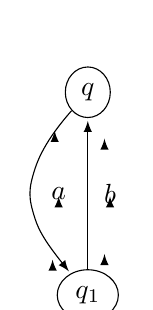
\begin{tikzpicture}[>=latex,line join=bevel,]
%%
\node (q) at (20.836bp,82.5bp) [draw,ellipse] {$q$};
  \node (q_1) at (20.836bp,9.5bp) [draw,ellipse] {$q_1$};
  \draw [->] (q) ..controls (10.35bp,70.587bp) and (4.4001bp,62.976bp)  .. (1.8362bp,55.0bp) .. controls (-0.61205bp,47.384bp) and (-0.61205bp,44.616bp)  .. (1.8362bp,37.0bp) .. controls (3.1625bp,32.874bp) and (5.395bp,28.845bp)  .. (q_1);
  \definecolor{strokecol}{rgb}{0.0,0.0,0.0};
  \pgfsetstrokecolor{strokecol}
  \draw (10.336bp,46.0bp) node {$a$};
  \draw (8.9136bp,69.589bp) node {$$};
  \draw (8.1621bp,23.245bp) node {$$};
  \draw [->] (q_1) ..controls (20.836bp,30.064bp) and (20.836bp,48.664bp)  .. (q);
  \draw (28.836bp,46.0bp) node {$b$};
  \draw (26.836bp,25.277bp) node {$$};
  \draw (26.836bp,66.794bp) node {$$};
%
\end{tikzpicture}

	\caption{LTS of $Blocked Q$} \label{fig:CompleteTraceEquivalenceBlockedQ}
	\endminipage\hfill
\end{figure}

\subsubsection{Failure equivalence}
Closely related to completed trace equivalence appears the failure equivalence, which solves preservation of equivalence by the blocking operator. The failure equivalence relates as many behaviors as possible, while preserving traces and deadlocks.

In order to define it, we introduce the set of failure pairs of a process, composed by a sequence of actions and some set of actions that (in some cases) cannot be performed after executing this trace.

\begin{definition} [Failure equivalence]
	Let $ A = (S, Act, \rightarrow, s_0 T) $ be a LTS. A set $ F $ is called a refusal set of a state $ t $ if:
	\begin{itemize}
		\item $ \forall a \in F \not \exists t’ $ such that $ t\xrightarrow{a}t’ $
		\item \cmark $ \in F \Rightarrow t \not \in T$
	\end{itemize}
	The set of failure pairs of t, $ FailurePairs(t) $ is defined as the minimal set of pairs that satisfies:
	\begin{itemize}
		\item $ (\varepsilon, F) \in FailurePairs(t) $ if $ F $ is a refusal set of $ t $.
		\item $($\cmark$, F) \in FailurePairs(t) \iff t \in T \wedge F $ is a refusal set of $ t $
		\item $t\xrightarrow{a}t’ \wedge (\sigma, F) \in FailurePairs(t’) \rightarrow (a\cdot\sigma, F) \in FailurePairs(t)$
	\end{itemize}
\end{definition} 
Again, two states are failure equivalent iff their failure pairs are the same, and two LTS are failure equivalent iff their initial states are.

Failure equivalence is used when we want to preserve deadlocks, some branching behavior and equivalence under application of the operators of the algebra. In practice, the size of the failure pairs is considerable, albeit empirically faster to compute than trace equivalence sets. \cite{valmari1995failure}

Next we present an example showing that the complete-trace equivalent processes in our previous example are not failure equivalent.

For the LTS of P, we observe that its set of failure pairs is $ \{(\varepsilon,U\subseteq\{b,c,$ \cmark $\}), (a,U\subseteq\{a,b,$\cmark$\}), (a,U\subseteq\{a,c,$\cmark$\}), \dots\} $; while for Q the set of failure pairs is $ \{(\varepsilon,U\subseteq\{b,c,$ \cmark $\}), (a,U\subseteq\{a,$\cmark$\}), \dots\} $, where the ellipsis represent pairs with traces of length greater or equal than two.

We clearly see that the pairs $ (a,\{b\}) $ and $ (a,\{c\}) $, among many other failure pairs of P, do not appear in Q's failure pairs set.

The next example showing a pair of failure equivalent processes will help us show the difference between the branching behavior captured by failure equivalence and the next equivalence: strong bisimulation.

Let be $ P = a·(b·$\cmark$+c·d·$\cmark$) + a·(f·$\cmark$+c·e·$\cmark$) $ and $ Q = a·(b·$\cmark$+c·e·$\cmark$) + a·(f·$\cmark$+c·d·$\cmark$) $,

\begin{figure} [H]
	\minipage{0.5\textwidth}
	\centering
	
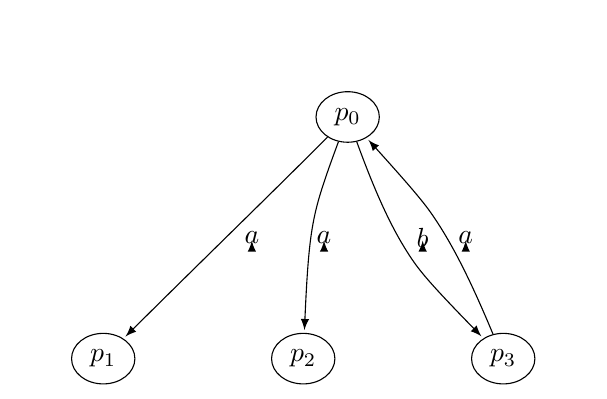
\begin{tikzpicture}[>=latex,line join=bevel,]
%%
\begin{scope}
  \pgfsetstrokecolor{black}
  \definecolor{strokecol}{rgb}{1.0,1.0,1.0};
  \pgfsetstrokecolor{strokecol}
  \definecolor{fillcol}{rgb}{1.0,1.0,1.0};
  \pgfsetfillcolor{fillcol}
  \filldraw (0.0bp,0.0bp) -- (0.0bp,123.0bp) -- (198.0bp,123.0bp) -- (198.0bp,0.0bp) -- cycle;
\end{scope}
  \node (p_2) at (99.0bp,18.0bp) [draw,ellipse] {$p_2$};
  \node (p_3) at (171.0bp,18.0bp) [draw,ellipse] {$p_3$};
  \node (p_0) at (115.0bp,105.0bp) [draw,ellipse] {$p_0$};
  \node (p_1) at (27.0bp,18.0bp) [draw,ellipse] {$p_1$};
  \draw [->] (p_3) ..controls (159.4bp,45.816bp) and (153.06bp,58.546bp)  .. (146.0bp,69.0bp) .. controls (143.06bp,73.344bp) and (139.64bp,77.725bp)  .. (p_0);
  \definecolor{strokecol}{rgb}{0.0,0.0,0.0};
  \pgfsetstrokecolor{strokecol}
  \draw (157.5bp,61.5bp) node {$a$};
  \draw [->] (p_0) ..controls (106.34bp,81.737bp) and (104.28bp,75.163bp)  .. (103.0bp,69.0bp) .. controls (101.48bp,61.698bp) and (100.53bp,53.686bp)  .. (p_2);
  \draw (106.5bp,61.5bp) node {$a$};
  \draw [->] (p_0) ..controls (86.081bp,76.067bp) and (64.992bp,55.697bp)  .. (p_1);
  \draw (80.5bp,61.5bp) node {$a$};
  \draw [->] (p_0) ..controls (125.23bp,77.03bp) and (131.05bp,64.297bp)  .. (138.0bp,54.0bp) .. controls (141.15bp,49.327bp) and (144.94bp,44.685bp)  .. (p_3);
  \draw (142.0bp,61.5bp) node {$b$};
%
\end{tikzpicture}

	\caption{LTS of $P$} \label{fig:FailureEquivalenceP}
	\endminipage\hfill
	\minipage{0.5\textwidth}
	\centering
	
\begin{tikzpicture}[>=latex,line join=bevel,]
%%
\node (q_7) at (99.0bp,18.0bp) [draw,ellipse] {$q_7$};
  \node (q_6) at (243.0bp,105.0bp) [draw,ellipse] {$q_6$};
  \node (q_5) at (171.0bp,105.0bp) [draw,ellipse] {$q_5$};
  \node (q_4) at (99.0bp,105.0bp) [draw,ellipse] {$q_4$};
  \node (q_3) at (27.0bp,105.0bp) [draw,ellipse] {$q_3$};
  \node (q_2) at (171.0bp,192.0bp) [draw,ellipse] {$q_2$};
  \node (q_1) at (99.0bp,192.0bp) [draw,ellipse] {$q_1$};
  \node (q_0) at (140.0bp,279.0bp) [draw,ellipse] {$q_0$};
  \node (q_8) at (171.0bp,18.0bp) [draw,ellipse] {$q_8$};
  \draw [->] (q_1) ..controls (75.07bp,162.75bp) and (58.964bp,143.74bp)  .. (q_3);
  \definecolor{strokecol}{rgb}{0.0,0.0,0.0};
  \pgfsetstrokecolor{strokecol}
  \draw (72.0bp,148.5bp) node {$b$};
  \draw [->] (q_4) ..controls (99.0bp,75.163bp) and (99.0bp,59.548bp)  .. (q_7);
  \draw (102.5bp,61.5bp) node {$e$};
  \draw [->] (q_0) ..controls (126.2bp,249.38bp) and (118.03bp,232.44bp)  .. (q_1);
  \draw (125.5bp,235.5bp) node {$a$};
  \draw [->] (q_1) ..controls (99.0bp,162.16bp) and (99.0bp,146.55bp)  .. (q_4);
  \draw (102.5bp,148.5bp) node {$c$};
  \draw [->] (q_0) ..controls (150.5bp,249.22bp) and (156.47bp,232.85bp)  .. (q_2);
  \draw (161.5bp,235.5bp) node {$a$};
  \draw [->] (q_5) ..controls (171.0bp,75.163bp) and (171.0bp,59.548bp)  .. (q_8);
  \draw (175.0bp,61.5bp) node {$d$};
  \draw [->] (q_2) ..controls (194.93bp,162.75bp) and (211.04bp,143.74bp)  .. (q_6);
  \draw (214.5bp,148.5bp) node {$f$};
  \draw [->] (q_2) ..controls (171.0bp,162.16bp) and (171.0bp,146.55bp)  .. (q_5);
  \draw (174.5bp,148.5bp) node {$c$};
%
\end{tikzpicture}

	\caption{LTS of $Q$} \label{fig:FailureEquivalenceQ}
	\endminipage\hfill
\end{figure}

Let us see that these two processes are failure-equivalent. Let us begin by computing the refusal sets for all nodes.

\begin{itemize}
	\item For process $ P $:
	\begin{itemize}
		\item $ p_0 $ has $ \{b, c, d, e, f, $ \cmark $\} $ and all its subsets as refusal sets,
		\item $ p_1 $ has $ \{a, d, e, f, $ \cmark $\} $ and all its subsets as refusal sets,
		\item $ p_2 $ has $ \{a, b, d, e, $ \cmark $\} $ and all its subsets as refusal sets,
		\item $ p_3 $ has $ \{a, b, c, d, e, f\} $ and all its subsets as refusal sets,
		\item $ p_4 $ has $ \{a, b, c, e, f$ \cmark $\} $ and all its subsets as refusal sets,
		\item $ p_5 $ has $ \{a, b, c, d, f$ \cmark $\} $ and all its subsets as refusal sets,
		\item $ p_6 $ has $ \{a, b, c, d, e, f\} $ and all its subsets as refusal sets,
		\item $ p_7 $ has $ \{a, b, c, d, e, f\} $ and all its subsets as refusal sets,
		\item $ p_8 $ has $ \{a, b, c, d, e, f\} $ and all its subsets as refusal sets.
	\end{itemize}
	\item For process $ Q $:
	\begin{itemize}
		\item $ q_0 $ has $ \{b, c, d, e, f, $ \cmark $\} $ and all its subsets as refusal sets,
		\item $ q_1 $ has $ \{a, d, e, f, $ \cmark $\} $ and all its subsets as refusal sets,
		\item $ q_2 $ has $ \{a, b, d, e, $ \cmark $\} $ and all its subsets as refusal sets,
		\item $ q_3 $ has $ \{a, b, c, d, e, f\} $ and all its subsets as refusal sets,
		\item $ q_4 $ has $ \{a, b, c, d, f$ \cmark $\} $ and all its subsets as refusal sets,
		\item $ q_5 $ has $ \{a, b, c, e, f$ \cmark $\} $ and all its subsets as refusal sets,
		\item $ q_6 $ has $ \{a, b, c, d, e, f\} $ and all its subsets as refusal sets,
		\item $ q_7 $ has $ \{a, b, c, d, e, f\} $ and all its subsets as refusal sets,
		\item $ q_8 $ has $ \{a, b, c, d, e, f\} $ and all its subsets as refusal sets.
	\end{itemize}
\end{itemize}

Next, we apply the definition to compute the failure pairs of the two initial states of these processes.

\begin{itemize}
	\item For the initial state $ p_0 $ of $ P $:
	\begin{itemize}
		\item $(\varepsilon, \{b, c, d, e, f, $ \cmark $\}) \in FailurePairs(p_0)$, and the same for all the subsets of this refusal,
		\item $(a, \{a, d, e, f, $ \cmark $\}) \in FailurePairs(p_0)$, and the same for all the subsets of this refusal,
		\item $(a, \{a, b, d, e, $ \cmark $\}) \in FailurePairs(p_0)$, and the same for all the subsets of this refusal,
		\item $(a·b, \{a, b, c, d, e, f\}) \in FailurePairs(p_0)$, and the same for all the subsets of this refusal,
		\item $(a·c, \{a, b, c, e, f$ \cmark $\}) \in FailurePairs(p_0)$, and the same for all the subsets of this refusal,
		\item $(a·c, \{a, b, c, d, f$ \cmark $\}) \in FailurePairs(p_0)$, and the same for all the subsets of this refusal,
		\item $(a·f, \{a, b, c, d, e, f\}) \in FailurePairs(p_0)$, and the same for all the subsets of this refusal,
		\item $(a·c·d, \{a, b, c, d, e, f\}) \in FailurePairs(p_0)$, and the same for all the subsets of this refusal,
		\item $(a·c·e, \{a, b, c, d, e, f\}) \in FailurePairs(p_0)$, and the same for all the subsets of this refusal.
	\end{itemize}
	\item For the initial state $ q_0 $ of $ Q $:
	\begin{itemize}
		\item $(\varepsilon, \{b, c, d, e, f, $ \cmark $\}) \in FailurePairs(q_0)$, and the same for all the subsets of this refusal,
		\item $(a, \{a, d, e, f, $ \cmark $\}) \in FailurePairs(q_0)$, and the same for all the subsets of this refusal,
		\item $(a, \{a, b, d, e, $ \cmark $\}) \in FailurePairs(q_0)$, and the same for all the subsets of this refusal,
		\item $(a·b, \{a, b, c, d, e, f\}) \in FailurePairs(q_0)$, and the same for all the subsets of this refusal,
		\item $(a·c, \{a, b, c, d, f$ \cmark $\}) \in FailurePairs(q_0)$, and the same for all the subsets of this refusal,
		\item $(a·c, \{a, b, c, e, f$ \cmark $\}) \in FailurePairs(q_0)$, and the same for all the subsets of this refusal,
		\item $(a·f, \{a, b, c, d, e, f\}) \in FailurePairs(q_0)$, and the same for all the subsets of this refusal,
		\item $(a·c·e, \{a, b, c, d, e, f\}) \in FailurePairs(q_0)$, and the same for all the subsets of this refusal,
		\item $(a·c·f, \{a, b, c, d, e, f\}) \in FailurePairs(q_0)$, and the same for all the subsets of this refusal.
	\end{itemize}
\end{itemize}

As we can see, $ FailurePairs(p_0) = FailurePairs(q_0) $, and therefore P and Q are failure equivalent.

\subsubsection{(Strong) bisimulation}

Bisimulation, or strong bisimulation, is the main equivalence relation used in process analysis, and also the finest of them. Bisimulation computation can be thought as the search of any possible difference which would cause their inequivalence. Therefore, intuitively, bisimulation equivalent processes are practically indistinguishable.

One of the reasons why bisimulation is more useful in practice than the other equivalences is that the algorithm for checking bisimulations are polynomial. However, it is also true that sometimes it becomes to fine, so that two processes that would ''behave the same´´ at a certain level of requiered observability, could be declared inequivalent.

\begin{definition} [Bisimulation]
	Let $ A = (S, Act, \rightarrow, s_0, T) $ be a LTS. Strong bisimulation is any symmetric binary relation $ R  \subseteq (S\times S) $, such that $ \forall s, t \in S$, if $s R t $:
	\begin{itemize}
		\item $ s\xrightarrow{a}s’ \Rightarrow \exists t’, t\xrightarrow{a}t’ \wedge s’ R t’ $
		\item $ t\xrightarrow{a}t’ \Rightarrow \exists s’, s\xrightarrow{a}s’ \wedge s’ R t’ $
		\item $ s \in T \iff t \in T $
	\end{itemize}
	
\end{definition}

Two states are strongly bisimilar iff there is a strong bisimulation relating them; and two LTS are strongly bisimilar iff their initial states are bisimilar.

An interesting property of strong bisimulation is that for every LTS there exists a unique minimal bisimilar equivalent LTS.

Reusing the previous example, we can see why P and Q are not strongly bisimilar. If that were the case, there would exist a bisimulation relating $ p_0 $ and $ q_0 $. But then, since we have that $ p_0 \xrightarrow{a}p_1 $, there must be some state $ q_\alpha $ bisimilar to $ p_1 $ (which must be $ q_1 $, because we have that $ p_1 \xrightarrow{b}p_3 $). But then, in a similar way, we obtain that $ p_4 $ and $ q_4 $ should be bisimilar, but this is clearly not the case, because the transitions leaving these states are totally different.

\subsubsection{Van Glabbeek linear time-branching time spectrum}

All of these process equivalences, and many others, were classified in a famous diagram that compared their strength by Van Glabbeek \cite{van1990linear}. The diagram displays the finest equivalences at the top and the coarsest at the bottom, and the arrows represent a refinement relation.

\subsection{Equivalences with internal actions}
The equivalences previously mentioned are not enough when the processes communicate and have internal actions. As we have seen, neither trace nor bisimulation equivalences consider the internal actions as special actions. As a consequence, these actions can be ''observed´´ as they would be ordinary actions. Therefore, we need some adequate, more sophisticated definitions in order to capture their desired internal characteristics.

\subsubsection{Weak trace equivalence}

Weak trace equivalence is the tau analogous to trace equivalence. In this case, the natural approach of simply ''ignoring´´ the execution of internal actions, but allowing them, is enough, and we collapse traces including internal actions in the usual way (i.e. as done in automata theory). As with trace equivalence, weak trace equivalence is defined by the equality of two sets of traces, in this case weak traces.

Weak trace equivalence is, as one could expect, the weakest of all equivalences that abstract internal behavior, not preserving deadlock nor branching behavior. The calculation of the smallest equivalent LTS is very hard; but in some cases, we can gain a better understanding of the behavior of a system by observing the weak trace equivalent system, and then changing the model if we find easily visible errors or apply a finer equivalence if necessary.

\begin{definition} [Weak trace equivalence]
	Let $ A = (S, Act, \rightarrow, s_0, T) $ be a LTS. The set of weak traces starting from a state $ t $, $ WTraces(t) $, is the minimal set that satisfies:
	\begin{itemize}
		\item $ \varepsilon \in WTraces(t) $
		\item \cmark $ \in WTraces(t) \iff t \in T $
		\item $ t\xrightarrow{a}t’, a\not = \tau \wedge \sigma \in WTraces(t’) \Rightarrow a\cdot\sigma \in WTraces(t) $
		\item $ t\xrightarrow{\tau}t’ \wedge \sigma \in WTraces(t’) \Rightarrow \sigma \in WTraces(t) $
	\end{itemize}
\end{definition}

While for traces, and thus for trace equivalence, we can obtain the corresponding weak version in a very natural (an easy) way, this is not certainly the case for bisimulation, where many technical butleties produce a collection of weak variants.

\subsubsection{Branching bisimulation}
With branching bisimulation, we introduce a simple way of abstracting the execution of $ \tau $ transitions when defining a bisimulation. The unobservability of  $ \tau $ actions is captured by allowing the matching state when ''replying´´ a $ \tau $ transition to be generated by another $ \tau $ transition (as in the strong case) but also doing nothing, since nothing is ''observed´´ when a $ \tau $ transition is executed.

\begin{definition} [Branching bisimulation]
	Let $ A = (S, Act, \rightarrow, s_0, T) $ be a LTS. The branching bisimulation in $ A $ is symmetric binary relation $ R  \subseteq (S\times S) $ such that $\forall s, t \in S$, if $ s R t $, then we have:
	\begin{itemize}
		\item If $ s\xrightarrow{a}s’$, then either:
		\begin{itemize}
			\item $ a = \tau \wedge s’ R t $
			\item There exists a sequence of (zero or more) $ \tau $ transitions $ t\xrightarrow{\tau^*}t’ $ such that $ s R t’ \wedge t’\xrightarrow{a}t'' $
		\end{itemize}
		\item $ s \in T $, there exists a sequence of (zero or more) $ \tau $ transitions $ t\xrightarrow{\tau^*}t’ $ such that $ s R t’ \wedge t’ \in T $
	\end{itemize}
\end{definition}

As usual, equivalence of two LTS represents just the equivalence of the corresponding initial states.

Since branching bisimulation does not observe $ \tau $ transitions, but neither their goal, it cannot observe $ \tau $ transitions that leave the state of the system(the so-called $ \tau $-loops). By removing $ \tau $-loops, branching bisimulation captures a notion of fairness, meaning that a system will never get stuck in an (unobservable) $ \tau $-loop.

A state with a $ \tau $-loop is called a divergent state.

\subsubsection{Divergence preserving branching bisimulation}
But sometimes, we are interested in distinguish between divergent and non-divergent states, so that this (basic) branding bisimilarity totally abstracts from divergence. For this purpose, we can extend the definition of branching bisimulation with one additional rule:
\begin{definition} [Divergence preserving branching bisimulation]
	Let R be a branching bisimulation relation. We say that the relation R is a divergence preserving branching bisimulation if, and only if, it satisfies the following condition:
	\begin{itemize}
		\item If $ s R t $ then there exists an infinite sequence $ s\xrightarrow{\tau}\cdots $ if and only if there is an infinite sequence $ t\xrightarrow{\tau}\cdots$.
	\end{itemize}
\end{definition}

\subsubsection{Rooted branching bisimulation}

The two previous bisimulations lack a very important property: congruence. We can see with these examples that, when combining branching bisimilar LTS’s, the resultant LTS’s may not be equivalent. 

%\begin{figure} [H]
%	\minipage{0.33\textwidth}
%	\centering
%	
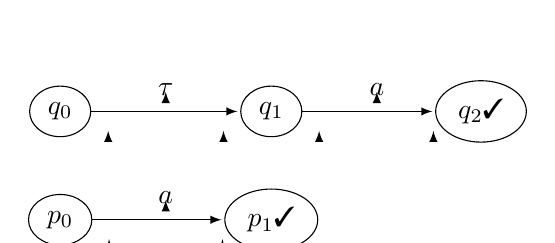
\begin{tikzpicture}[>=latex,line join=bevel,]
%%
\begin{scope}
  \pgfsetstrokecolor{black}
  \definecolor{strokecol}{rgb}{1.0,1.0,1.0};
  \pgfsetstrokecolor{strokecol}
  \definecolor{fillcol}{rgb}{1.0,1.0,1.0};
  \pgfsetfillcolor{fillcol}
  \filldraw (0.0bp,0.0bp) -- (0.0bp,67.0bp) -- (174.0bp,67.0bp) -- (174.0bp,0.0bp) -- cycle;
\end{scope}
  \node (q_2) at (163.0bp,51.0bp) [draw,ellipse] {$q_2\text{\cmark}$};
  \node (p_1) at (87.5bp,12.0bp) [draw,ellipse] {$p_1\text{\cmark}$};
  \node (q_1) at (87.5bp,51.0bp) [draw,ellipse] {$q_1$};
  \node (p_0) at (11.5bp,12.0bp) [draw,ellipse] {$p_0$};
  \node (q_0) at (11.5bp,51.0bp) [draw,ellipse] {$q_0$};
  \draw [->] (q_0) ..controls (33.945bp,51.0bp) and (52.037bp,51.0bp)  .. (q_1);
  \definecolor{strokecol}{rgb}{0.0,0.0,0.0};
  \pgfsetstrokecolor{strokecol}
  \draw (49.5bp,59.0bp) node {$\tau$};
  \draw (28.789bp,45.0bp) node {$$};
  \draw (70.298bp,45.0bp) node {$$};
  \draw [->] (p_0) ..controls (34.202bp,12.0bp) and (51.916bp,12.0bp)  .. (p_1);
  \draw (49.5bp,20.0bp) node {$a$};
  \draw (29.102bp,6.0bp) node {$$};
  \draw (69.917bp,6.0bp) node {$$};
  \draw [->] (q_1) ..controls (109.8bp,51.0bp) and (127.77bp,51.0bp)  .. (q_2);
  \draw (125.5bp,59.0bp) node {$a$};
  \draw (104.72bp,45.0bp) node {$$};
  \draw (145.87bp,45.0bp) node {$$};
%
\end{tikzpicture}

%	\caption{Branching bisimilar a's} \label{fig:BranchingBisimulationAes}
%	\endminipage\hfill
%	\minipage{0.33\textwidth}
%	\centering
%	
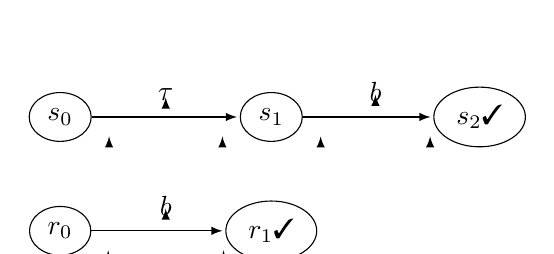
\begin{tikzpicture}[>=latex,line join=bevel,]
%%
\begin{scope}
  \pgfsetstrokecolor{black}
  \definecolor{strokecol}{rgb}{1.0,1.0,1.0};
  \pgfsetstrokecolor{strokecol}
  \definecolor{fillcol}{rgb}{1.0,1.0,1.0};
  \pgfsetfillcolor{fillcol}
  \filldraw (0.0bp,0.0bp) -- (0.0bp,71.0bp) -- (174.0bp,71.0bp) -- (174.0bp,0.0bp) -- cycle;
\end{scope}
  \node (r_0) at (11.5bp,12.0bp) [draw,ellipse] {$r_0$};
  \node (s_0) at (11.5bp,53.0bp) [draw,ellipse] {$s_0$};
  \node (s_2) at (162.5bp,53.0bp) [draw,ellipse] {$s_2\text{\cmark}$};
  \node (s_1) at (87.5bp,53.0bp) [draw,ellipse] {$s_1$};
  \node (r_1) at (87.5bp,12.0bp) [draw,ellipse] {$r_1\text{\cmark}$};
  \draw [->] (r_0) ..controls (33.945bp,12.0bp) and (52.037bp,12.0bp)  .. (r_1);
  \definecolor{strokecol}{rgb}{0.0,0.0,0.0};
  \pgfsetstrokecolor{strokecol}
  \draw (49.5bp,21.0bp) node {$b$};
  \draw (28.789bp,6.0bp) node {$$};
  \draw (70.298bp,6.0bp) node {$$};
  \draw [->] (s_0) ..controls (34.202bp,53.0bp) and (51.916bp,53.0bp)  .. (s_1);
  \draw (49.5bp,61.0bp) node {$\tau$};
  \draw (29.102bp,47.0bp) node {$$};
  \draw (69.917bp,47.0bp) node {$$};
  \draw [->] (s_1) ..controls (110.05bp,53.0bp) and (126.93bp,53.0bp)  .. (s_2);
  \draw (125.0bp,62.0bp) node {$b$};
  \draw (105.27bp,47.0bp) node {$$};
  \draw (144.68bp,47.0bp) node {$$};
%
\end{tikzpicture}

%	\caption{Branching bisimilar b's} \label{fig:BranchingBisimulationBes}
%	\endminipage\hfill
%\end{figure}

To solve this problem, the rooted version of branching bisimulation is introduced.
\begin{definition} [Rooted branching bisimulation]
	Let $ A = (S, Act, \rightarrow, s_0, T) $ be a LTS. A rooted branching bisimulation is a branching bisimulation such that, $ \forall s,t \in S$, if $ s R t $ then:
	\begin{itemize}
		\item $ s\xrightarrow{a}s’ \Rightarrow \exists t’, t\xrightarrow{a}t’ \wedge s’$ is branching bisimilar to $ t’ $.
	\end{itemize}
\end{definition}

As opposed to the previous bisimulation definitions, this one is not defined recursively. This is because the only nedded change concerns the first transition of the equivalent states, as those reached after the first transition are only required to be branching bisimilar, and not rooted branching bisimilar.

We can notice that if we were to define these bisimulations in a recursive way, we would simply end up with the definition of strong bisimulation!

\subsubsection{(Rooted) Weak bisimulation}
Finally, we introduce the ''plain´´ weak forms of bisimulation. In this case part of the ''branching information´´ that branching bisimulation had to preserve needs not to be preserved anymore, and thus we obtain a coarser semantics to the handling of $ \tau $ actions.
\begin{definition} [Weak bisimulation]
	Let $ A = (S, Act, \rightarrow, s_0, T) $ be a LTS. A weak bisimulation is a symmetrical binary relation $ R $ such that $\forall s, t \in S$, with $ s R t $:
	\begin{itemize}
		\item If $ s\xrightarrow{a}s’ $, either
		\begin{itemize}
			\item $ a = \tau  \wedge s’ R t $
			\item $ \exists t\xrightarrow{\tau^*}\xrightarrow{a}\xrightarrow{\tau^*}t’ $ such that $ s’ R t’ $
		\end{itemize}
		\item $ s \in T \Rightarrow \exists t\xrightarrow{\tau^*}t’, t’ \in T $
	\end{itemize}
\end{definition}

\begin{definition} [Rooted weak bisimulation]
	Let $ A = (S, Act, \rightarrow, s_0, T) $ be a LTS. A rooted weak bisimulation on A is a weak bisimulation relation $ R $ which when $s R t$, also satisfies:
	\begin{itemize}
		\item $ s\xrightarrow{\tau}s’  \Rightarrow \exists  t\xrightarrow{\tau}\xrightarrow{\tau^*}t’ $ such that s’ is weakly bisimilar to t’
	\end{itemize}
\end{definition}


\subsection{Basic criteria when choosing an equivalence relation}
After defining all these (certainly many) relations between LTSs, we will briefly discuss which one to choose, depending on our intended goals, using some simple examples that intuitively show the reasons why the indicated one would be the most adequate in each case.

\subsubsection{The criteria to use when we do not have any internal steps}
In LTSs without internal steps, there will be a clear statement:
\begin{center}
	Strong bisimulation is always safe.
\end{center}

The reason why this is true is that, strong bisimilarity only relates processes that are behaviorally indistinguishable, and therefore when we identify two bisimilar systems there is no risk of losing any information.

In the opposite end of the spectrum, we have trace equivalence, where the LTSs are reduced much more, easily losing some branching information. As a consequence, we cannot use trace equivalence when interested in the identification of deadlocks. But traces are still enough to characterize some reachability properties, thus remaining useful to establish safety properties.

An intermediate choice would be failure equivalence, preserved by the application of the usual operators in process algebras. This equivalence is highly useful as it has been empirically shown to be efficient to calculate \cite{valmari1995failure}, and with absence of non-deterministic parallelism failure and trace equivalences are practically equivalent.

For example, if we were to implement the embedded system of a modern vehicle, we would expect that no component deadlocks; for instance, when we need to use the electronically controlled break, or when the parking assistance system steers the wheel. For these systems, if there were no non-determinism, we could analyze the failure equivalent LTS to verify whether or not deadlocks could appear, but trace equivalence would not be enough, for the reasons discussed above.

\subsubsection{The criteria to take into account when considering internal steps}

With internal steps, divergence preserving branching bisimulation would be the safe option playing the role of strong bisimulation in the previous case.

Now, plain branching bisimilarity (without preserving divergences), would be enough as far as liveness properties that could be (theoretically) lost when divergences appear are not important, or when we assume that those liveness properties (mainly bounded bypass, as we are dealing with potential infinite loops) will be guaranteed by other means.

Moreover, in practice weak bisimulation empirically works as branching bisimulation in many cases, so it can be safely used as an alternative.

But since weak trace equivalence removes all the internal actions, the (exact) branching behavior can be lost in some cases, so we should carefully study if weak bisimilarity is enough depending on the exact information that we would need to preserve.

As an example, let us think of a cryptographic communication protocol, in which the internal actions are not interesting to us by themselves, and we only want to know if there is a way the password (think of it as a private key, like in RSA) could be leaked to an intruder. In this case, we do not care about tau-loops, so we can use plain branching bisimulation. Instead, we could not use weak bisimulation, nor weak trace equivalence, because of the high parallelism (and thus non-determinism) in the system.

Another example could be the modeling of a routing protocol, like RIP (which we will model and verify later on in this work), where we would like to ensure that the routing is set up correctly always, and that the system does not get stuck computing divergent calculation (as it occurs in RIPv1). This latter property of absence of livelocks is related to the (possible) presence of $ \tau  $ loops, so that divergence preserving branching bisimulation should be imposed to remain safe.
%TODO Actually model RIP :lazy:

\clearpage

\section{Modal Logics}
Up until now, we have shown how to model a concurrent system using a high-level (algebraic) syntax and the semantic LTS representation, and how equivalences preserve properties that we want to verify. Next, we will concentrate on the formalism that allows to model properties, and verify them over the LTS previously produced. These formalism are the modal logics. In this work, we will briefly introduce the Hennessy-Milner logic and an important extension, the $ \mu $-calculus.
\subsection{Hennessy-Milner Logic}
The Hennessy-Milner logic follows the syntax of prepositional logic, extending it with two quantifier-like  modal operators, related to the usual first-order $ \exists $ and $ \forall $. Its defining grammar is as follows:

\begin{center}
	$ \phi $ ::= $true$ $ \vert $ $false$ $ \vert $ $\neg \phi$ $ \vert $ $\phi \wedge \phi$ $ \vert $ $\phi \vee \phi$ $ \vert $ $\phi \rightarrow \phi$ $ \vert $ $\langle a \rangle\phi$ $ \vert $ $[a]\phi $
\end{center}

Any logic statement, applied to a certain state, can only evaluate to True or False. The usual logic operators $ \vee $, $ \wedge $, $ \neg $, have their usual meanings. Also, the implication operator is defined to ease the writing of formulas, as it can be rewritten with $ \wedge $ and $ \neg $. \\
The main modal operator is the diamond modality, $ \langle a\rangle $. $ \langle a\rangle\phi $ evaluates to True when \emph{there exists} an $ a $-transition from the current state that leads to a state where $ \phi $ is true. The dual box modality, $ [a]\phi$, represents if \emph{every} transition from the current state ends in a state that satisfies $ \phi $.

Because our main goal is to analyze the dynamics of concurrent systems (via their semantic LTS representation), it is clear that these two modal operators are crucial to state the required properties.

As with first-order logic, the modalities here verify that not $ \langle\rangle\phi = []\neg\phi $, $ \neg[]\phi = \langle\rangle\neg\phi $.

As usual, we will say that the labeled transition system satisfies the modal formula $ \iff $ it is satisfied by the initial state.

\subsection{$\mu$-calculus}
The previous definition of the Hennessy-Milner will not be enough for us, as we have a rather problematic structure in our some of our transition systems: recursive definitions. To solve this limitation, we must extend the modal logic thus introducing \emph{fixed-point} modalities.

A fixed-point p of a function f is an element that verifies the equation $ p = f(p) $. In our case, the functions will be recursive logic formulas; and the domain, the set of states of the LTS. In general, these fixed-points will not be unique, but with respect to set inclusion. Because we care about sets of states, we can distinguish two especially interesting fixed-points: the minimal and maximal fixed-points.

The minimal fixed-point, $ \mu X.\phi(X) $, is satisfied by the states in the smallest set of states where phi is satisfied. Similarly, the maximal fixed point, $ \nu X.\phi(X) $, is satisfied by the states in the largest set of states where phi is satisfied.

Taking $ \phi(X)=X $ we obtain a trivial example:
\begin{center}
	$ \mu X. X $ \\
	$ \nu Y. Y $
\end{center}

where $ \mu X. X $ is obviously equivalent to false and $ \nu Y. Y $ equivalent to true, because the empty set and the full set of states are the smallest and largest solutions of the equation $ X = X $, respectively.

A more complex example would be the condition that needs to be satisfied to get sound mutual exclusion locks, which are described by the formula:

\begin{center}
	$ \nu X. \nu Y. ((\langle lock\rangle Y \vee [!lock]X) \wedge (\langle unlock\rangle X \vee [true] Y)) $
\end{center}

This formula states that, if the lock is locked, no other locking action will be performed until it is unlocked again. In our Appendix ? you can find the verification of this property on some lock implementations.

%TODO verification of lock

Another way to understand the fixed-point modalities is by considering the minimal fixed-point as a recursive function that is satisfiable in a certain finite number of steps. On the other hand, the maximal fixed point would be true after infinitely many steps. These two metaphors bring us the notions of liveness and safety, respectively.

A liveness property of a condition ensures that the condition will successfully occur within a finite number of steps. Dually, a safety property ensures that the condition will not happen within an infinite number of steps. For example, the convergence of a certain algorithm can be thought as a liveness property, whereas the absence of deadlocks would be a safety property.

In order to use fixed-point modalities, we first need to prove the existence of fixed-points. If the fixed-point variable in a fixed-point modality appears evenly preceded by negations, then there exists a unique solution to the modality. You can find a proof of this property in our Appendix ?.
%TODO proof of monotony

To use the full potential of fixed-point modalities, we have to combine minimum and maximum fixed-points. In this we obtain new capabilities, such as stating that a property must happen if it is available a potentially infinite number of times, or if some other action only happens a finite number of times. The latter is a notion of fairness. We can find interesting fairness properties in multiqueued systems like gas stations or supermarkets, where the systems should guarantee that a customer will get served in some finite time.

Fairness for an \textbf{enter} action can be specified by the following formula:

\begin{center}
	$ \nu X. \mu Y. ((\langle enter\rangle Y \vee [true]X) \wedge (\neg \langle enter \rangle X \vee [true] Y)) $
\end{center}

This formula states that for every state there is a finite sequence of states where the action \textbf{enter} cannot be performed. This is useful, paired with the previous formula, to verify that a mutual exclusion lock is fair (i.e. every thread using the lock has the opportunity to \textbf{enter} its critical section, without getting live-locked).

\subsection{Regular formulas}
If we consider the actions of a concurrent system as an alphabet $\Sigma$, we can define the regular expressions over said alphabet. Using these newly defined “transition languages”, we can make the formulas more meaningful.
The action languages are defined, as usual, with the following grammar:
\begin{center}
	$ af $ ::= $\alpha$ $ \vert $ $true$ $ \vert $ $false$ $ \vert $ $ \overline{af}$ $ \vert $ $af \cap af $ $ \vert $ $af \cup af$
\end{center}
Here, $ true $ and $ false $ represent \emph{any} actions and \emph{no} actions, respectively. In other words, $ true $ is the full language of words; and $ false $, the empty language. The negation $ \overline{af} $, union $ \cup $, and intersection $ \cap $ of action languages have the usual meaning.

To be formally correct, we must define the $ \mu $-calculus over action languages. Because actions only appear in the modalities, we only need to define:
\begin{center}
	$ \langle L\rangle\phi = \bigvee_{\alpha\in L} \langle a\rangle\phi $\\
	$ [L]\phi = \bigwedge_{\alpha\in L}[a]\phi $.
\end{center}
Based on these languages, we can define the regular expressions with the common operators:
\begin{center}
	$ R $ ::= $\varepsilon$ $ \vert $ $af$ $ \vert $ $R\cdot R$ $ \vert $ $ R + R$ $ \vert $ $R^* $ $ \vert $ $R^+$
\end{center}

But, why do we extend modalities to work with regular expression? The answer is simple, even if adding regular expressions does not add semantic capabilities to $ \mu $-calculus, it lets us define formulas that would otherwise be quite large and complex. For example, if we have to check that a property is satisfied when a (finite) even number of $ a $ actions are executed, we would write the following formula:

\begin{center}
	$ \nu X.[a][a](\phi\wedge X)$
\end{center}

With regular expression, knowing that the language describing words with a finite even number of $ a $ actions is $ a^* $, we would rewrite the formula above as:

\begin{center}
	$ [a*]\phi $
\end{center}

These two formulas are equivalent, but the latter is much more concise and understandable, and compositionally even bigger formulas collapse to much smaller sizes.

\subsection{Checking Modal Formulas}
Once we have defined the formulas we want to check, and the labeled transition systems where they should be checked, there are multiple ways to check the validity of a formula, but we will show here the direct method applied to LTSs.
%TODO comment direct method
For Hennessy-Milner formulas, the procedure is quite simple. By labeling the states of the LTS with subformulas of the logical statement, we can verify the satisfiability at the initial state iff its label is the complete formula.
This process is defined like this:
\begin{itemize}
	\item First label all states with \textit{true}.
	\item For each subformula $\phi$, for each state $s$:
	\item Label $s$ with $\neg \phi$ if it is not labeled with phi
	\item Label $s$ with $\phi \wedge \psi$ if it is labeled with $\phi$ and with $\psi$
	\item Label $s$ with $\phi \vee \psi$ if it is labeled with $\phi$ or with $\psi$
	\item Label $s$ with $\langle a \rangle\phi$ if there is a transition $s\xrightarrow{a}s’$ and $s’$ satisfies $\phi$
	\item Label $s$ with $[a]\phi$ if for all transitions $s\xrightarrow{a}s’$, $s’$ satisfies $\phi$
\end{itemize}

Because in Hennessy-Milner formulas there is no recursion, the set subformulas is finite, and thus the algorithm terminates.

In order to check mu-calculus formulas, extending the former algorithm will not suffice. When handling minimal fixed points $ \mu X.\phi(X) $, we will label the states with all subformulas of phi, including X. In the case of maximal fixed points $ \nu X.\phi(X) $, the process is reversed, initially labeling the states with X and removing it when the state does not verify phi after the iterations stabilize.

We will prove that formula ? is satisfied by the sample lock. %TODO SAMPLE LOCK proof of concept

\clearpage

\section{Model Analysis}
In previous chapters we have seen the equivalence relations between Labeled Transition Systems. That technique is very powerful, but requires us to translate the processes to their semantic representations. In this chapter we lay down the derivation rules that can be applied to formulas of process algebra to conclude whether they are equivalent or not.

The main rules used are the induction over data types, the Recursive Specification Principle (RSP), and Koomen's fair abstraction rule. Except for the latter, the first two rules relate process formulas that are bisimilar. For Koomen's rule, two choices are given, one rule for branching bisimulation and another for weak bisimulation.

These tools are used to check if an equation is provable. This will be used to create what is called a process linear form, with a method called linearization. We will not go into much detail about linearization, only that it is used as an intermediate step to compute efficiently strong bisimulation, see \cite{HIRSHFELD1996143}.
\subsection{General Derivation Rules}
\begin{table}
	\centering
	\begin{tabular}{ c l }
		\infer{\Gamma \cup \{p = q\} \vdash p = q}{} & start \\
		\infer{\Gamma \vdash p = p}{} & reflexivity \\
		\infer{\Gamma \vdash p = q}{\Gamma \vdash q = p} & symmetry \\
		\infer{\Gamma \vdash p = r}{\Gamma \vdash p = q & \Gamma \vdash q = r} & transitivity\\
		\infer{\Gamma \vdash p_1·p_2 = q_1·q_2}{\Gamma \vdash p_1 = q_1 & \Gamma \vdash p_2 = q_2} & congruence\\
		\infer{\Gamma \vdash p = q}{\Gamma \vdash p·x = q·x} & extensionality\\	
		\infer{\Gamma \vdash \lambda x:D. p = \lambda x:D. q}{\Gamma \vdash p = q} & abstraction\\	
		\infer{\Gamma \vdash \lambda x:D. p = \lambda y:D. (p[x:=y])}{} & $ \alpha-conversion $\\	
		\infer{\Gamma \vdash (\lambda x:D. p) q = p[x:=q]}{} & $ \beta-conversion $\\	
	\end{tabular}
\end{table}


To anyone who has worked with derivation rules on theory of programming languages, these rules are self-explanatory. Nevertheless, we will give a succinct explanation for the more complex ones, finishing with a more practical approach.

Here, $\Gamma$ represents the context, the statements above the horizontal bar are the hypotheses and the ones below the bar are the conclusions. When we write x $ \not \in \Gamma $, we are describing that, as a requirement for the rule to be true, x should not be a free variable on the context $ \Gamma $.

The congruence rule states that equality is preserved after concatenating processes (with the dot operator).
The extensionality rule states that, if x is not a free variable, then we can decompose it from a previous equality, implying the equality of the preceding terms.
The abstraction rule states that, if x is not a free variable, then we can surround equal elements by a lambda over x while preserving equality.
The $ \alpha $ conversion states that we can rename the free variable of a lambda expression, as long as we rename it on the inner terms as well.
The $ \beta $ conversion states that we can apply an element to a lambda expression by substituting all appearances of the free variable for the argument.
The other rules are deduced from standard first-order logic.

For logical formulas, rules are very straightforward. The only caveat to notice is that we transform every logical statement to compositions of $ (true = false) $, $ \Rightarrow $ (which is a functionally complete set for propositional logic, see \cite{Vaughan1942-VAURWW}) and $ \forall $.

\begin{table}
	\centering
	\begin{tabular}{ c l }
		\infer{\Gamma \cup \{\phi\} \vdash \phi}{} & generalized start \\
		\infer{\Gamma \vdash \phi}{\Gamma \vdash true = false} & principle of explosion \\
		\infer{\Gamma \vdash \phi \Rightarrow \psi}{\Gamma \cup \{\phi\} \vdash \psi} & $ \Rightarrow $ introduction\\
		\infer{\Gamma \vdash \phi \Rightarrow \psi}{\Gamma \vdash \phi \Rightarrow \psi & \Gamma \vdash \phi} & $ \Rightarrow $ elimination\\
		{\infer{\Gamma \vdash \forall x:D. \phi}{\Gamma \vdash \phi}}, $ x \notin \Gamma $ & $ \forall $ introduction\\	
		\infer{\Gamma \vdash \phi[x:=p]}{\Gamma \vdash \forall x:D. \phi} & $ \forall $ elimination\\	
		\infer{\Gamma \vdash \forall x:D. \phi = \forall y:D. (\phi[x:=y])}{} & $ \alpha$-conversion for $ \forall $\\	
	\end{tabular}
\end{table}

\subsection{Induction over Data Types}
This rule will let us work over the structure of data types to prove equality.
Let D be some structured data type (or sort, in mCRL2 nomenclature). The following rules stand:

\begin{table}[h]
	\centering
	\begin{tabular}{ c l }
		\infer{\Gamma \vdash \phi}{\{\Gamma \vdash \bigwedge_{D_i = D}{\phi[x := x_i]} \Rightarrow \phi[x := c_i (x_1,\dots,x_n)] \vert c_i $ is a constructor of $ D\}} & induction
	\end{tabular}
\end{table}

This states that, for a formula $ \phi $ to be true for a sort $ D $, it must be true for every possible constructor of $ D $ and every combination of their parameters.

This induction rule works with booleans and natural numbers as well as user defined types, finite or infinite.

\subsection{Recursive Specification Principle}
The RSP will be the tool to prove equality of recursive process equations. To ensure the uniqueness of the possible solution, we have a condition similar to the one applied in the modalities of $ \mu $-calculus, called guardedness.
To properly formalize the RSP, we shall define process operators.

A process operator is a mapping with domain $D$, where $D$ can be the set of processes $P$ or the set of mappings from some tuple of data types to $P$. Therefore, a process operator can be applied to a simple process or one that depends on data. Thus, we can think of process operators as mappings $D\longrightarrow D$.
\begin{definition}[Guarded process]
	A process variable $X:D\longrightarrow P$ is guarded in a process $p$ if, and only if:
	\begin{itemize}
		\item If $p = \delta $ or $p = \alpha $, then X occurs guarded in $p$.
		\item If $p = p_1 + p_2 $, $ p_1 || p_2 $, $ p_1 | p_2 $, $ c\rightarrow p_1 <> p_2 $, $ p_1 << p_2 $, then X occurs guarded in $ p_1 $ and $ p_2 $.
		\item If $p = \sum_{d:D} p_1 $, $ p_{1}^ct$, $ c \longrightarrow p_1 $, $ t >> p_1 $, $ p_1 << t $, $ \Gamma_{C}(p_1) $,$ \nabla_{V}(p_1) $, $ \Delta_{B}(p_1) $, $ \rho_{R}(p_1) $, the X occurs guarded in $ p_1 $.
		\item If $p =  p_1 . p_2 $, $ p_1 ||\_ p_2 $, then X occurs guarded in $ p_1 $.
	\end{itemize}
	
\end{definition}

The RSP ensures that a recursive equation $X =  \Psi X$ with, $ \Psi $ a process operator, can only have one solution if, and only if $X$ is guarded in $ \Psi $. This is equivalent, in a way, to saying that $ \Psi $ can only have one fixed point. A proof of this fact can be viewed in annex ?.

The RSP is stated formally in this rule:

\begin{table}[h]
	\centering
	\begin{tabular}{ c l }
		\infer{\Gamma \vdash X = Y}{\{\Gamma \vdash X = \Psi X & Y = \Psi Y} & recursive specification principle
	\end{tabular}
\end{table}

\subsection{Koomen's Fair Abstraction Rule}

Koomen's fair abstraction rule (KFAR) will help us prove process equalities when using hiding operators. In order to do this correctly, we have to ensure that by hiding actions we do not modify process behaviors. The property required is fairness. This is, the branches affected by the hiding operators must let other actions happen eventually. KFAR was an idea found implicitly in Koomen's signaling modeling \cite{KOOMEN19851}, but was first explicitly written as a rule in \cite{BAETEN1987129}.

Two different rules exist, one for branching bisimulation and another for weak bisimulation.

\begin{table}[h]
	\centering
	\begin{tabular}{ c l }
		\infer{\Gamma \vdash \tau · \tau_{\{i\}}(X) = \tau · \tau_{\{i\}}(Y)}{\Gamma \vdash X = i·X + Y} & KFAR (branching bisimulation) \\
		\infer{\Gamma \vdash \tau_{\{i\}}(X) = \tau · \tau_{\{i\}}(Y)}{\Gamma \vdash X = i·X + Y} & KFAR (weak bisimulation) \\
	\end{tabular}
\end{table}

Let it be noted that Groote-Mousavi's axioms for rooted branching and weak bisimulation imply both KFAR rules.

\subsection{Linearization, Grebach form and applications}

A linear process equation (LPE) is process equation that satisfies some ``shape'' conditions. With normalized forms like the one linear process equations have, analysis and manipulation becomes easier and standardized.

In LPEs, the left-hand side variable is the only variable used in the right-hand side. This variable is always preceded by one action in the right-hand side, thus making the LPE a guarded recursive specification.

\begin{definition} [Linear process equation]
	An LPE is a recursive process equation with the following shape:
	\begin{align}
			X(d:D) = &\sum_{i\in I}\sum_{e_i:E_i} c_i (d,e_i) \rightarrow\alpha_i (d,e_i)·X(g_i(d,e_i)) \\
			& + \sum_{j\in J}\sum_{e_j:E_j} c_j (d,e_j) \rightarrow\alpha_{\delta_j}(d,e_j)
	\end{align}
	
	Where $ I,J \subset \mathbb{N} $, $ \{E_k\}_{k\in K \subset \mathbb{N}} $ are sorts,  $ \{c_k\}_{k\in K \subset \mathbb{N}} $ are parameterized conditions, $ \{\alpha_k\}_{k\in K \subset \mathbb{N}} $ are parameterized actions, $ \{\alpha_{\delta_k}\}_{k\in K \subset \mathbb{N}} $ are parameterized actions or $ \delta $, and $ \{g_k\}_{k\in K \subset \mathbb{N}} $.
\end{definition}

Usually we can assume that $ \alpha_{\delta_k} $ is $ \delta $.

Linearization is a multiple step process. Starting from a guarded recursive specification we transform it to a Greibach normal form, with a intermediate pre-Greibach normal form.

Because this process is cumbersome, details are to be seen in \cite{Groote:2014:MAC:2628007} and \cite{Baeten:1993:DBE:174130.174141}.

\subsubsection{$ \tau $-priorization}
Process parallelization produces space state explosion. When using parallel operators in combination to hiding operators, most transitions tend to be $\tau$-transitions. To reduce unnecessary transitions, where choices cannot be made because of near $ \tau $-transitions, we use $ \tau $-priorization. We will assume $ \tau $-confluence, that is, there are no $ \tau $-loops.

For an LTS A, a $ \tau $-priorization of A is another LTS, which transition set is a subset A's transition set, where for every state $ s $, if there are transitions $ s\xrightarrow{\tau}s' $ and $ s\xrightarrow{a}s'' $, the non-$ \tau $ transition is removed.

\begin{thm}
	Let $ A_1 $ and $ A_2 $ be LTSs. If $ A_2 $ is a $ \tau $-priorization of $ A_1 $, then $ A_1 $ and $ A_2 $ are branching bisimilar.
\end{thm}

\section{Modeling time}

\subsection{Historical context}
Dealing with time has been a problematic topic in the algebraic description of processes. On \cite{Baeten1991}, Baeten and Bergstra discuss how to extend (or actually generalize) the definition of ACP (Algebra of Communicating Processes, a precursor of $ \mu $CRL2), where they point out the necessity of a formal generalization and operational semantics for timed processes in order to be able to verify properties without limitations. Other proposals involve the use of discrete timings, as in \cite{hennessy1995process} and \cite{baeten1996discrete}. As we can see, there is not an absolute consensus in whether use discrete time with step delays, which lacks the descriptive dynamism of an arbitrary slicing of time steps; or real valued time (which presents difficulties if no limit in precision is imposed (in recursive processes with decreasing time margins).

\subsection{From actions to timed actions}

As we defined at the beginning of this text, actions are the atom of our processes, and thus take no time to execute. By adding a timestamp to actions, we will be stating that such actions must be performed at that exact point in time. Actions are marked with a timestamp, as we have seen in the algebraic definition, as $ a^c t $, where $ t $ is the time in a dimensionless representation. The fact that timed actions must occur in an specific moment brings us to the main constraint of time actions: there must be time coherence between the executed actions of a trace. This translates on invalid or incoherent traces to end in a deadlock state.

In $ \mu CRL2 $, timestamps following actions in timed actions represent time points in a globally scoped timeline. Therefore we must ensure that we define correctly timed actions so no unintended time blocks happen. One consequence of introducing this kind of timing system is that, because inconsistent traces end up in deadlocks, many of the possible traces produced by the combinatorial explosion in parallelization of processes disappear, as many of these traces do not satisfy the requirements due to impossible reorderings of timed actions. As an example, we can see that, for actions $ a^c 1 $, $ b^c 2 $, and $ c^c 3 $, the only possible ordering is $ a·b·c $ in their respective times, and that if we were to write the process $ a^c 1 || b^c 2 || a^c 3 $, the only proper trace would be the one we just wrote before.

Between timed actions, time must run. When time runs, we are not performing any action. This is what we call idling. Behaviorally, between two sequential timed actions (or multiactions) we consider that the system idles. When defining a system, we can specify that there can be idling at a given time. If at the same time there exists another action that must execute at that time, then two things might happen: we perform the action or we idle and skip that action.

\subsection{Timed Labeled Transition Systems}

To define timed LTS's, we only need to consider adding the two concepts mentioned before: time coherence and idling.

For time coherence, we will forbid that two sequential transitions execute action in reverse time order. This is the so called progress requirement, as time must strictly increase after each action.

\begin{center}
 s $ \xrightarrow{a}_{t} $ s' $ \xrightarrow{'a}_{'t} $ s'' $ \Rightarrow t < t $
\end{center}

For idling, we must correctly represent that if an action will occur at a given time, the system can idle until that time comes. Furthermore, if a system can idle up to a given time, it can obviously idle up to nearer points of time. This is called the density requirement, as the ability to idle is dense in time intervals.

To represent idling, a new relation is introduced, indicating with s $ \leadsto_{t} $ that from state s we can idle up to time t. Note that this relation does only involve one state, meaning that no actual state change.

The transformation from an untimed LTS to a timed one is quite simple, we only have to introduce the progress and density requirements as follows: assign time 0 to the initial state of the LTS and give arbitrary positive time points to terminal states. Then assign times to each transition, giving increasing timestamps in each transition.

\subsection{Behavioral equivalence revamped}

To work with timed LTS's, we need to also extend the definitions of our behavioral equivalences. We will only indicate the slight differences and show the formal definition.

\subsubsection{Timed trace equivalence and timed weak trace equivalence}

The definition of the Traces(s) set changes slightly. When an idle relation comes from a state, we must add the timestamp of the idling in the new TTraces (timed traces) set. In creating the traces, we must note that actions have to be timestamped and considered when equating traces.

\begin{definition} [Timed trace equivalence]
	Let $ A = (S, Act, \rightarrow, \leadsto, s_0, T) $ be a timed LTS. The set of timed traces starting from $ s \in S$, $ TTraces(s) $, is the minimal set that satisfies:
	\begin{itemize}
		\item $ \varepsilon \in TTraces(s) $
		\item \cmark $ \in TTraces(s) \iff s \in T $
		\item $ s\leadsto_t \Rightarrow t \in TTraces(s) $
		\item $ s\xrightarrow{a}_t s’ \wedge \sigma \in TTraces(s’) \Rightarrow a^c_t\cdot\sigma \in TTraces(s) $
	\end{itemize}
\end{definition}

\begin{definition} [Timed weak trace equivalence]
	Let $ A = (S, Act, \rightarrow, \leadsto, s_0, T) $ be a timed LTS. The set of timed weak traces starting from $ s \in S$, $ WTTraces(s) $, is the minimal set that satisfies:
	\begin{itemize}
		\item $ \varepsilon \in WTTraces(s) $
		\item \cmark $ \in WTTraces(s) \iff s \in T $
		\item $ s\leadsto_t \Rightarrow t \in WTTraces(s) $
		\item $ s\xrightarrow{a}_t s’, a^c_t\not = \tau \wedge \sigma \in WTTraces(s’) \Rightarrow a^c_t\cdot\sigma \in WTTraces(s) $
		\item $ s\xrightarrow{\tau}_t s’ \wedge \sigma \in WTTraces(s’) \Rightarrow \sigma \in WTraces(s) $
	\end{itemize}
\end{definition}

\subsubsection{Timed strong and branching bisimulations}

For timed strong bisimulation, only considering timestamps and idling will suffice, the definition does not change much more than that.

\begin{definition} [Timed strong bisimulation]
	Let $ A = (S, Act, \rightarrow, \leadsto, s_0, T) $ be a timed LTS. The strong bisimulation is a symmetric binary relation $ R  \subseteq (S\times S) $ where $ s, t \in S, s R t $ if, and only if:
	\begin{itemize}
		\item $ s\xrightarrow{a}s’ \Rightarrow \exists t’, t\xrightarrow{a}t’ \wedge s’ R t’ $
		\item $ t\xrightarrow{a}t’ \Rightarrow \exists s’, s\xrightarrow{a}s’ \wedge s’ R t’ $
		\item $ s \in T \iff t \in T $
	\end{itemize}
	
\end{definition}

In the case of timed branching bisimulation, things get more complicated. If we recall the definition of branching bisimulation, a transition on one state must be simulated by a series of $ \tau $ transitions and a proper transition in the other state. Here, we must make the timings of these intermediate $ \tau $ transitions match with the concept of bisimulation. For this, a timed branching bisimulation relation is parameterized by a time variable, representing a relation where related elements use that time as a starting referential point. On top of that, we must also add support for idling.

\begin{definition} [Timed branching bisimulation]
	Let $ A = (S, Act, \rightarrow, \leadsto, s_0, T) $ be a timed LTS. For $ t \in \Re $ $ t \geq 0 $, $ t $-timed branching bisimulation is a symmetric binary relation $ R_t  \subseteq (S\times S) $ where $ s, u \in S, s R u $ if, and only if:
	\begin{itemize}
		\item If $ s\xrightarrow{a}_{t’}s’$ with $ t’ > t $, then $ \exists t = t_0 < t_1 < \dots < t_n < t_{n+1} = t’ $ such that either:
		\begin{itemize}
			\item $ a = \tau \wedge u = u_0 \xrightarrow{\tau}_{t_1} u_1 \xrightarrow{\tau}_{t_2} \dots \xrightarrow{\tau}_{t_n} u_n \leadsto_t’ , \forall i \in N, w \in \Re, 0 \leq i \leq n \wedge t_i \leq w < t_{i+1} \wedge s R_w u_i \wedge s’ R_{t’} u_n $
			\item $ a \not = \tau \wedge u = u_0 \xrightarrow{\tau}_{t_1} u_1 \xrightarrow{\tau}_{t_2} \dots \xrightarrow{\tau}_{t_n} u_n \xrightarrow{a}_{t’} u’ , \forall i \in N, w \in \Re, 0 \leq i \leq n \wedge t_i \leq w < t_{i+1} \wedge s R_w u_i \wedge s’ R_{t’} u’ $
			\item $ \exists t’, t\xrightarrow{a}t’ \wedge s’ R t’ $
		\end{itemize}
		\item If $ s\leadsto_{t’}  $, $ \exists t = t_0 < t_1 < \dots < t_n < t_{n+1} = t’ $ such that $ u = u_0 \xrightarrow{\tau}_{t_1} u_1 \xrightarrow{\tau}_{t_2} \dots \xrightarrow{\tau}_{t_n} u_n \leadsto_t’ , \forall i \in N, w \in \Re, 0 \leq i \leq n \wedge t_i \leq w < t_{i+1} \wedge s R_w u_i \wedge s R_{t’} u_n $
		\item $ s \in T \iff u \in T $
	\end{itemize}
\end{definition}

\subsection{Timed processes and timed formulas}

The extension of timed processes is simple, we just need a way of labeling actions with their respective timestamps. For this, the $ at $ operator is introduced, and is written as we have already seen in timed actions. For equational definition of processes, the $ at $ operator cannot be used, for it can only be used in atomic actions. To represent that an equation has a time dependence, we must pass a time parameter as an argument of the parameterized equation. For this to be useful, timestamps must have the possibility of being variable and depend on an external variable.

Much like timed processes, we will use the $ at $ operator following actions to represent timestamps in $ \mu $ calculus formulas. Another additions to $ \mu $ calculus are the introduction of two new basic elements, $ delay $ and $ yaled $, used to represent existance of (or lack thereof) idling. The $ delay $ operator represents that a delay occurs, meaning that no action is performed; its counterpart, yaled, expresses the concept that an action must occur, and that the system cannot idle indefinitely. Both elements can be followed by timestamps just like timed actions do.

\section{mCRL2}

mCRL2 is a specification language and tool for modeling and specification of concurrent systems. mCRL2 specification language is a one to one transformation from process algebra explained here, assigning operators and keywords for basic operations like choice and sequential composition and complex operations like parallel composition, hiding, sum, etc.

\subsection{Language specification}

\subsubsection{mCRL2 process specification language}

System specification is encapsulated in a single \textbf{.mcrl2} extension file. 

A mCRL2 file usually starts with \textbf{sort} declarations, similar to Haskell's type declaration. Sorts can be constructors without parameters, or general constructors with possibly multiple parameters, both with a preceding \textbf{struct} keyword. Sort declarations can act as aliases for other sorts, mainly mappings from sorts to sorts. Finally, sorts can be unspecified with an incomplete declaration. Unspecified sorts can later be specified by declaring constants.

mCRL2 adopts a similar typing system as Haskell, adding cartessian products of sorts.


Parameter variables need not be previously declared as variables, but must be free variables unless binding is wanted. Self-reference is permitted in parameterized constructors.

\begin{center}
	\textbf{sort} Card = \textbf{struct} heart | tile | clover | pike; \\
	\textbf{sort} Tree = \textbf{struct} leaf(A) | node(Tree, A, Tree); \\
	\textbf{sort} Message = \textbf{struct} m(source:IP, destination:IP, content:List(Char))
\end{center}

Sorts can be followed by \textbf{map} declarations and \textbf{eqn} definitions.

Map declarations specify the type of the mapping. To define the behavior of mappings, equation definitions are required. Equation definitions have pattern matching capabilities, and have proven to be very useful with constructed sorts. Variables for equation definitions must be declared previously with a \textbf{var} statement.

\begin{align}
	\textbf{map} & left : Tree -> Tree; \\
	\textbf{var} & l, r : Tree; \\
	& a : A;
	\textbf{eqn} & left(node(l,a,r)) = l; \\
	\textbf{map} & data = Tree -> Tree; \\
	\textbf{var} & l, r : Tree; \\
		& a : A; \\
	\textbf{eqn} & data(node(l,a,r)) = a;  \\
	& data(leaf(a)) = a;
\end{align}

After specifying sorts and sort functions, we predeclare all actions that will appear in our specification. As some actions are parameterized, we must state the cartessian product of the parameters. Actions created as a result of communication operators have to be declared here as well.

\begin{align}
	\textbf{act} & send, receive, communicate : Message; \\
				 & turn\_on, turn\_off; \\
\end{align}

Next, we will define all the required recursive specifications. We can use processes to modularize behavior inside a system. Process declaration is preceded by a \textbf{proc} keyword. Each process is defined by an equation. The left-hand side of the equation is composed by the process variable, in which we also declare parameters and their types. In the right-hand side we use process variables without explicitly writing parameter types.

\begin{tabular}{c c c}
	\textbf{proc} &  & \\
	 & Client(inputQueue : List(Message), outputQueue : List(Message) = sum m:Message. recieve(m).Client(m |> inputQueue), outputQueue) & \\
	 &  & + send(rhead(outputQueue)).Client(inputQueue, tail(outputQueue)) ;
\end{tabular}

Lastly, we have to declare the initial instance to verify. This part is preceded by the \textbf{init} keyword. Usually, the \textbf{init} part is composed by some processes in parallel, with a combination of communication, hiding and allow operators.

\begin{center}
	\textbf{init} allow({communicate},
	comm({send|receive->communicate},
	Client([],[]) || Client([],[])
	)
	);
\end{center}

Processes are defined using process algebra operators. Process operators in mCRL2 are written in the following manner:

\begin{tabular}{c c}
	Process algebra operator & mCRL2 operator \\
	\hline
	Alternative composition (Choice) & + \\
	Sequential composition & . \\
	Deadlock & delta \\
	Conditional operator & \underline{condition} -> \underline{then} <> \underline{else} \\
	Sum operator & sum \underline{variable}:\underline{sort}.\underline{process} \\
	Parallel composition & \underline{process} || \underline{process} \\
	Synchronization operator & \underline{action} | \underline{action} \\
	Communication operator & comm(\underline{set of pairings and transformations},\underline{process}) \\
	Allow operator & allow(\underline{list of actions},\underline{process}) \\
	Blocking operator & block(\underline{list of actions},\underline{process}) \\
	Renaming operator & comm(\underline{set of renamings}, \underline{process}) \\
	Hiding operator & hide(\underline{set of actions}, \underline{process})
\end{tabular} 

\subsubsection{mCRL2 $ \mu $-calculus language}

To specify $ \mu $-calculus formulas, we must write separate files from our .mcrl2 files. Their extension does not matter, as the tool does not process them by themselves. Following the examples packaged with the tool, we will use the .mcf extension, which we presume means $ \mu $-calculus formula.

The syntax of a .mcf file is quite simple, the formula to be evaluated is written directly in $ \mu $-calculus syntax. 

$ \mu $-calculus's written syntax is the following:

\begin{tabular}{c c}
	$ \mu $-calculus element & mCRL2 written form \\
	\hline
	true & \textit{true} \\
	false & \textit{false} \\
	$ \mu . X \phi $ & \textit{mu} X. \underline{phi} \\
	$ \nu . X \phi $ & \textit{nu} X. \underline{phi} \\
	$ \forall d:D.\phi $ & \textit{forall} d:D. \underline{phi} \\
	$ \exists d:D.\phi $ & \textit{exists} d:D. \underline{phi} \\
	$ \phi \Rightarrow \psi $ & \underline{phi} => \underline{psi} \\
	$ \phi \vee \psi $ & \underline{phi} $ \vert \vert $ \underline{psi} \\	
	$ \phi \wedge \psi $ & \underline{phi} \&\& \underline{psi} \\
	$ [a] \phi $ & [a] \underline{phi} \\
	$ \langle a\rangle \phi $ & <a> \underline{phi} \\
	$ \neg \phi $ & ! \underline{phi} \\
\end{tabular} 

\subsubsection{Other internal languages}

The mCRL2 toolset has many utilities and transformations we can apply to our process modeling. Many of those transformations cover sections mentioned in this text, and that have their own syntax.

The only ones worth mentioning are the textual representation of (non)parameterized boolean equations, which can be output in the last phase of model verification, that is, when we are combining both model specification and $ \mu $-calculus formula.

This transformation is automatically done by the toolset, and we have not needed to modify and of the produced .pbes files in our examples.

\subsection{Using mCRL2}

During the development of this project, we used the mCRL2 toolset over Windows with its original GUI. This has proven to facilitate the process of calling the programs that form the whole toolset. There are other releases for OSX and Linux-based systems, but in the following steps we will show how to validate and analyze in Windows. Experience may vary in other platforms. We start by downloading the Windows installer from \href{http://www.mcrl2.org/web/user_manual/download.html}{http://www.mcrl2.org/web/user\_manual/download.html}.

After installing, we open the program mcrl2-gui. This window will appear:

\includegraphics[width=0.8\textwidth, keepaspectratio]{img/mCRL2/mcrl2-intro.png}

We must navigate through the file system to where our files reside.

\includegraphics[width=0.8\textwidth, keepaspectratio]{img/mCRL2/mcrl2-files.png}

We see there are two .mcrl2 files, \textit{Needham-SchrederPublicKeyProtocol.mcrl2} and \textit{Needham-SchrederPublicKeyProtocolFixed.mcrl2}. There are also two .mcf files, \textit{compromisedCommunication.mcf} and \textit{correctComunication.mcf}.

We will proceed to check that \textit{Needham-SchrederPublicKeyProtocol.mcrl2} verifies the $ \mu $-calculus formula \textit{compromisedCommunication.mcf}.

We start by right-clicking the .mcrl2 file, and click in the transformation mcrl22lps, which will transform our mCRL2 process model to its standard Grebach Linear Process equation System. A new tab will appear in the right section of the interface. We can see all the available options for this tool. In this case, we recommend to set the linearization method to ``stack'' for models that have an extremely large state-space unless the host computer lacks sufficient resources. Once run, a new file with extension .lps will be produced.


Right-clicking on the .lps file, we are given several options. In the analysis menu, we can get information about the LPS with the tool lpsinfo, which will show basic statistics about the structure of the LPS. Below, by using the command lpspp we can pretty-print the LPS back to mCRL2 language, this is useful if we want to see what is the produced Grebach form. In the transformation menu, we are given the choice to apply many transformations, many of which simplify and make more efficient further verification steps. Because most do not advance to the next step, we will only mention the ones we will use, lps2lts and lps2pbes.
lps2lts transforms the linear process system to its equivalent labeled transition system. This transformation is useful because an LTS acts as a good visual representation of how a small system behaves. This tool produces a file with .lts extension.
lps2pbes will be the tool we usually use in this case, transforming the linear process system to a behaviorally equivalent set of parameterized boolean equations, following an algorithm similar to the one we described before. In this tool we use as input the $ \mu $-calculus formula as well, getting a .pbes file in return.

On a .pbes file, we can finally check if our model behaves like we would want it to. To do this, we right-click into the analysis menu, clicking in the tool pbes2bool.

On a .lts file, we can visualize the labeled transition system. There are a few tools for this, but the two most useful have been ltsview and ltsgraph.
ltsgraph creates a 2D/3D image with nodes as circles and transitions as labeled arrows. This representation is quite useful as the tool lets us move nodes and distribute them around the canvas with ``physics-based'' algorithms. Nodes can be modified by color and size, and an option for 3D display can be chosen to enable better visualization of large but clustered LTS's. The graph can be exported to image and XML files for later use.

\includegraphics[width=0.8\textwidth, keepaspectratio]{img/mCRL2/mcrl2-ltsgraph.png}

ltsview displays the LTS as a tubular tree shape, where sequential actions are represented by cylindrical columns and multiple transitions to different nodes are represented by conical trunks widening where most states are. Final states are represented with spheres, indication no outward transitions exist. In this tool we can select to mark deadlocks and terminating nodes, states and transitions, and walk action traces step by step, visualizing the states we traverse in the 3D figure.

\includegraphics[width=0.8\textwidth, keepaspectratio]{img/mCRL2/mcrl2-ltsview.png}

One last tool is ltscompare, which implements equivalence checking algorithms for the behavioral equivalences shown in this text. This tool will compare two .lts files, identifying if they are is any counter-example to its equivalence. The accepted behavioral equivalences are:

\begin{itemize}
	\item Strong bisimilarity.
	\item Branching bisimilarity.
	\item Divergence-preserving branching bisimilarity.
	\item Weak bisimilarity.
	\item Divergence-preserving weak bisimilarity.
	\item Trace equivalence.
	\item Weak trance equivalence.
	\item Simulation equivalence (not discussed here).
\end{itemize}

Using this comparison tool, we can check correct behavioral implementation by checking against a model of the specification. 
\newpage
\begin{appendices}
In the following appendices, we show examples of modeling and verification using the mCRL2 toolset. Source code for the models and resulting files from the analyses can be found in the following GitHub repository: ?.
%TODO: GitHub
\section{Needham-Schroeder protocol}
The Needham-Schroeder protocol is an authentication protocol for potentially vulnerable networks. It relies on the security provided by encryption to safely send authentication keys through the network. There are two versions of the protocol, one based on symmetric encryption and one based on asymmetric public-private key encryption, both introduced by Roger Needham and Michael Schroeder at Xerox Palo Alto in the late 70's\cite{Needham:1978:UEA:359657.359659}. Unfortunately, for both versions of the protocol there were attacks that compromised the intended safety\cite{Denning:1981:TKD:358722.358740}\cite{Lowe:1995:ANP:219887.219895}. Be noted that, for the public-private key encryption version, a long 17 years passed until the error was found and a solution was given, showcasing the importance of automated verifications. 

We will show how the public-private key version of Needham-Schroeder's protocol can be compromised by a man-in-the-middle attack, where the attacker (hereinafter the intruder) impersonates the originator of a communication presumed safe. After showing how it can be attacked, we will add the modifications needed to solve the error, as shown in \cite{Lowe:1995:ANP:219887.219895}, and prove that it now is, in fact, a safe protocol in regards to man-in-the-middle attacks.

\subsection{Description of the protocol}

The public-private key version of the Needham-Schroeder protocol defines a set of operations (similarly to an API), and an order in which they must be performed between two entities that wish to authenticate their identities. As the entity who starts the communication is the one which starts the protocol, from now on we will call this entity the client; and the other entity, which receives the starting protocol message, will be called the server. The idea of the protocol is sending nonces (unique arbitrary numbers) generated by the client and the server, using encryption to prevent prying eyes. The encrypted nonces are passed back and forth once, so that both client and server know that the other party is who it says to be. This is possible because, assuming the unlikelihood of a coincidence of nonces, an intruder would need to decrypt the messages and return the nonces to their respective entities, which would imply a breach in the encryption algorithm.

\subsection{Attack pattern and how to fix it}

The intruder will perform a man-in-the-middle attack (i.e. the intruder acts as an intermediary between the client and the server). Once the client has connected to the intruder (by error or with the help of malware or phishing), the intruder then would impersonate the server with the client's connection and vice-versa. Because the client made a connection with the intruder, the intruder is able to decrypt the nonce of the client and send it to the server; but it will not be able to decrypt the incoming nonce of the server, as it is encrypted with the public key of the client. By passing the encrypted message to the client and getting the confirmation back, the intruder is now able do decrypt and get the server's nonce, thus successfully completing the attack.

The solution is quite simple: the nonce that is sent by the server must have appended the servers identification. Because this message is encrypted with the client's key, the intruder is not able to modify it. The client would then notice the difference between the identification of its connection (the intruder) and the message it has received.

\subsection{Modeling and verification}

This appendix's files are located in the Needham-Schroeder folder. The files named \texttt{``Needham-SchroederPublicKeyProtocol''} refer to the original version of the protocol, whereas \texttt{``Needham-SchroederPublicKeyProtocolFixed''} refer to the fixed protocol. Two $ \mu $-calculus formulas are provided: \texttt{compromisedCommunication}, which checks if the intruder can compromise the authentication, and \texttt{``correctCommunication''}, which checks that both originator and destination of the communications have, as far as they individually know, succeeded on authenticating.

In our model, we ignore the existence of an authentication server and assume that the name lookup has already been done in some way. This is valid, as the underlying problem of the protocol does not involve the intervention of the authentication server. Another important paradigm applied is to try to build a solution-agnostically model, that is, without biasing the model to produce the known solution. For this, the intruder is modeled as a process that can perform the operations defined by the protocol, but without any implicit order, thus allowing a bigger and more realistic generated state-space. The only restrictions in which the intruder is constrained is that it can only perform communications to the destinations that make sense. Also, encrypted data that cannot be decrypted by the intruder is only passed through, thus preserving the safety provided by the encryption algorithm.

After linearising the process specification, we can produce its LTS. We can see that the state-space generated is quite small: only 24 states and 33 transitions, with 3 deadlocks, 2 of which represent a failure in the communication at the start (this is the case when the intruder communicates with the server before the client has sent any information to the intruder). There is only one trace where the intruder wins (modulo ordering of the actions we use to show correct protocol communication).

\begin{figure}
\centering
\includegraphics[width=0.4\textwidth, keepaspectratio]{img/Needham-Schroeder/state-LTSview.png}
\caption{Original LTS in hierarchical form}\label{ltsNSView}
\end{figure}
\begin{figure}
\includegraphics[width=\textwidth,keepaspectratio]{img/Needham-Schroeder/state-LTSgraph.png}
\caption{Original LTS with attack trace in red}\label{ltsNSGraph}
\end{figure}

Because this problem has such a small state-space, further simplification using behavioral equivalences is not needed.

Applying the $ \mu $-formula that checks if the intruder can win, we find that, as we expected, the formula is true. The tool also gives us the justification, in terms of the satisfied parameterized boolean equation that deduce the result. These formulas are harder to read than the actions they represent, but if the state-space is small one can use the \texttt{ltsgraph} tool with the ``Show state labels'' option and follow this trace by hand.
\begin{figure}[h]
\begin{lstlisting}
1: X(1,client,client,client_n,client_n,client,none_n,none_n,none,false,1,client,client_n,client,intruder,1,client,client,client_n,client_n,client,client)
4: Subst:true X(1,client,client,client_n,client_n,client,client_n,none_n,client,false,2,client,client_n,client,intruder,1,client,client,client_n,client_n,client,client)
5: Subst:true X(1,client,client,client_n,client_n,client,client_n,none_n,client,false,2,client,client_n,client,intruder,2,server,intruder,client_n,server_n,client,intruder)
8: Subst:true X(2,intruder,client,client_n,server_n,client,client_n,none_n,client,false,2,client,client_n,client,intruder,3,client,client,client_n,client_n,client,intruder)
9: Subst:true X(1,client,client,client_n,client_n,client,client_n,none_n,client,false,3,client,server_n,intruder,intruder,3,client,client,client_n,client_n,client,intruder)
11: Subst:true X(1,client,client,client_n,client_n,client,client_n,server_n,client,false,4,client,client_n,client,client,3,client,client,client_n,client_n,client,intruder)
\end{lstlisting}
\caption{Attack trace result of applying \texttt{``compromisedCommunication''}}
\end{figure}

Now, using the model of the fixed version of Needham-Schoreder's protocol, we get a slightly smaller LTS, with only 13 states and 14 transitions. We can simulate the execution with LTSView and in fact we can see that there are only 3 traces (modulo reordering of actions), one in which client and server reject the authentication, and other two where the intruder fails to use the protocol API correctly. Therefore, we can conclude that the addition of the server's identity on the confirmation message sent by the client.

\begin{figure}
\centering
\includegraphics[width=0.4\textwidth, keepaspectratio]{img/Needham-Schroeder/fixed-state-LTSview.png}
\caption{Fixed LTS in hierarchical form}\label{ltsNSFixedView}
\end{figure}
\begin{figure}
\centering
\includegraphics[width=\textwidth, keepaspectratio]{img/Needham-Schroeder/fixed-state-LTSgraph.png}
\caption{Fixed LTS with no attack trace}\label{ltsNSFixedGraph}
\end{figure}

After applying the previous $ \mu $-formula we obtain a negative result.

\section{TCP timed modeling}

The Transmission Control Protocol is one of the most used protocols on the Internet. It ensures transmission of data preventing data loss and preserving the order in which the receiving end get the information. In order to ensure this properties, the protocol defines a series of procedures that both parties of a communication must apply. These procedures encompass retransmission of data and retransmission of acknowledgement messages, with the use of timers and a strict timeout standard.

Here, we model an abstraction of the Transmission Control Protocol, with the purpose of showing that no packet of data is lost, and that every packet read by the receiver is correctly ordered. We focused on the usage of timers and modeling them with our timed process algebra. Due to limitations on our computer, the verification of these conditions was not possible, as it seemed to make no progress on the phase of solving the parameterized boolean equation system. Nevertheless, the model is represented by a valid mCRL2 file and could be verified with the appropiate equipment.

The files of this model are located on the TCP folder.

\section{Mutual exclusion locks: Tie-Breaker and Ticket algorithms}

In concurrent programming, parallel algorithms are used to improve performance over sequential implementations. A parallel algorithm runs over multiple threads of execution, sharing memory locations as a way to communicate between one another. Because totally parallelized memory accesses are not deterministic, we need a way to prevent parallelization of some parts of the code: the problem of mutual exclusion. A lock is a mechanism that limits access to some parts of code. Once a thread has locked a lock, no other thread may lock it, thus stopping until the lock has been unlocked. There are many ways of implementing locks, the most commonly used nowadays based on hardware-supported operations. Here we will model and verify mutual exclusion on the traditional implementations of locks, mainly the tie-breaker and ticket algorithms.

\subsection{Tie-breaker algorithm}
The tie-breaker, as defined for two threads, consists on an ``in'' flag for each thread and a shared ``last'' variable, which indicates which thread entered the locking procedure last. The two threads mark themselves as last threads to enter the lock, and actively wait until the they are the other thread has started the locking algorithm or the other thread's ``in'' flag is down. Once this condition is satisfied, the thread is ensured to have exclusive execution of the following code until its ``in'' flag is disabled again.

For modeling this algorithm, the pseudocode from \cite{andrews2000foundations} was used. While verifying the model, a flaw was found in the book's pseudocode: the order in which the lock sets up the ``in'' and ``last'' variables changes the behavior of the lock. In the book, the ``in'' flag is enabled and then the ``last'' variable is updated. When doing this, the lock does not ensure mutual exclusion, because the order in which the active wait checks the two conditions must not be the same as these assignments. Using the tools we are able to identify the trace of execution that led to the unsatisfied exclusiveness property and figure out a simple way to fix it.

The files of this appendix are located on the ``Tie-breaker'' folder. Here we have two models: the model as it was originally defined in \cite{Peterson1981115}, in the file ``tiebreaker-peterson''; and the flawed model based on the pseudocode from \cite{andrews2000foundations}, in the file ``tiebreaker-andrews''. We additionally have two $ \mu $-formulas to check, one for exclusiveness and one for fairness. We will show that this algorithm is only fair when using a weakly fair scheduler.

When applying the exclusiveness $ \mu$-formula to the flawed LTS, we get the following counterexample:

\begin{figure}[h]
\begin{lstlisting}
1: X1(1,c1,c1,c1,c1,c1,c1,true,c1,true,1,c1,c1,c1,c1,c1,c1,true,c1,true,false,false,c1)
4: Subst:false   X(1,c1,c1,c1,c1,c1,c1,true,c1,true,1,c1,c1,c1,c1,c1,c1,true,c1,true,false,false,c1)
6: Subst:false   X(2,c1,c1,c1,c1,c1,c1,true,c1,true,1,c1,c1,c1,c1,c1,c1,true,c1,true,false,false,c1)
9: Subst:false   X(2,c1,c1,c1,c1,c1,c1,true,c1,true,2,c1,c1,c1,c1,c1,c1,true,c2,true,false,false,c2)
19: Subst:false   X(2,c1,c1,c1,c1,c1,c1,true,c1,true,3,c1,c1,c1,c1,c1,c1,true,c1,true,false,true,c2)
32: Subst:false   X(2,c1,c1,c1,c1,c1,c1,true,c1,true,4,c1,c1,c1,c1,c1,c1,false,c1,true,false,true,c2)
50: Subst:false   X(2,c1,c1,c1,c1,c1,c1,true,c1,true,5,c1,c1,c1,c2,c2,c2,true,c1,false,false,true,c2)
80: Subst:false   X(3,c1,c1,c1,c1,c1,c1,true,c1,true,5,c1,c1,c1,c2,c2,c2,true,c1,false,true,true,c2)
114: Subst:false   X(4,c1,c1,c1,c1,c1,c1,true,c1,true,5,c1,c1,c1,c2,c2,c2,true,c1,false,true,true,c2)
147: Subst:false   Y(4,c1,c1,c1,c1,c1,c1,true,c1,true,6,c1,c2,c2,c1,c1,c1,true,c1,false,true,true,c2)
180: Subst:false   Y(5,c1,c1,c1,c1,c1,c1,true,c1,false,6,c1,c2,c2,c1,c1,c1,true,c1,false,true,true,c2)
\end{lstlisting}
\caption{Counterexample of exclusiveness on Andrews's Tie-breaker implementation}
\end{figure}

Now we can look for a trace where the actions \texttt{lock(c1)} and \texttt{lock(c2)} happen one after the other. After applying divergence-preserving branching bisimulation on the LTS, we find that a trace that satisfies this is:

\begin{figure}[h]
\begin{lstlisting}
writeTurn(c1).writeTurn(c2).write(c2,true).read(c1,false).write(c1,true).readTurn(c2).read(c2,true).readTurn(c2).lock(c1).lock(c2)
\end{lstlisting}
\caption{Trace breaking exclusiveness on Andrews's Tie-breaker implementation}
\end{figure}

Once again, on the correction of the algorithm the exclusiveness formula is true, as can be checked using the toolset.

\subsection{Ticket algorithm}
The ticket algorithm relies on ordering the accesses to the lock, giving a ``ticket'' with a number to each thread that starts the locking mechanism. The algorithm also needs a variable to hold the current turn in the sequence of tickets: the thread with a ticket equal to the turn is the one which will complete the locking process. 

To achieve an ordered sequence of tickets, an atomic way of increasing a variable is needed. This is possible by using another lock, but that solution is highly inefficient. We instead will use a hardware-supported atomic operation: fetch-and-add. The fetch-and-add operation (FA) atomically returns the value of a variable and increases its value by one. After obtaining a ticket, a thread actively waits until it is its turn. After completing the locked code, the thread just needs to increase the value of the turn variable, so that the next thread can enter the exclusive section.


As with the previous lock, the pseudocode the pseudocode from \cite{andrews2000foundations} was used. In this case, after checking the $ \mu $-formula for exclusiveness, an affirmative response was given, meaning that this implementation is correct.

The files of this model are located on the ``Ticket'' folder.

While making the model, several values for the number of threads were tested. As one would expect, the more threads we have, the larger the resultant state-space gets. In figure \ref{statesTicket} a chart of the states of the LTS versus the number of threads is given. As we can seen, the growth seems to be around two orders of magnitude for each new thread, indicating a exponential dependency between the size of the LTS and the number of threads.

\begin{figure}
\begin{tikzpicture}
\begin{axis}
  \addplot+ [sharp plot,] coordinates {
      (2,195),(3,6922),(4,381949),(5,30689306)
  };
\end{tikzpicture}
\caption{States vs threads in the ticket algorithm}\label{statesTicket}
\end{figure}

To take into account, for two and three threads, it took the tool less than a second to produce the LTS; for four threads, it took about half an hour; and for five threads, it took seven hour. The last LTS couldn´t even be saved, as the computer ran out of its 16GB of RAM before it could be written to memory.

Not minding the original size of the LTSs, we will consider the size of their divergence-preserving branching bisimulating. In figure \ref{dpbbStates} we can see that the number of states decreases considerably. Unfortunately, the LTS for five threads could not be saved because of hardware limitations.

\begin{figure}
\begin{tikzpicture}
\begin{axis}
  \addplot+ [sharp plot,] coordinates {
      (2,13),(3,40),(4,145)
  };
\end{tikzpicture}
\caption{States vs threads after divergence-preserving branching bisimulation}\label{dpbbStates}
\end{figure}

\begin{figure}
\centering
\includegraphics[width=0.4\textwidth, keepaspectratio]{img/Ticket/n4dpbb.png}
\caption{LTS for n=4 in ticket after divergence preserving branching bisimulation}\label{n4dpbb}
\end{figure}

\section{Dining philosopher's problem}

The dining philosopher's problem is a classic problem in the study of concurrent systems and deadlocks. At a dining table, five philosophers are sitting wanting to eat, but there are only five forks available. For this problem we have to assign the forks in a manner such that every philosopher can eat and no ``deadlock'' situation occurs.

The solution is quite simple, every philosopher grabs the fork on his right side and then the fork on the left side, except for the last philosopher, who does this reversing the order.

The files of this model are located on the ``Philosophers'' folder.

The resulting LTS has 2164 states, which decrease to 532 when applying divergence-preserving branching bisimulation, and further decreasing to 32 once weak trace equivalence is used. The LTS has a ovoid shape, where every possible combination of \texttt{eat} and \texttt{think} actions is represented by a state.

\begin{figure}
\centering
\includegraphics[width=0.4\textwidth, keepaspectratio]{img/Philosophers/wt.png}
\caption{LTS for the philosophers problem after weak trace equivalence}\label{phiwt}
\end{figure}

\end{appendices}


%===============================================================================
%===============================================================================
%===============================================================================
\newpage
\bibliographystyle{plain}
\bibliography{references}{}


\end{document}

